% MSc thesis style for TU Delft Embedded Networked Systems Group.

% MIT License
%
% Copyright (c) 2023 TU Delft Embedded Systems Group and Casper Dennis van Wezel.
%
% Permission is hereby granted, free of charge, to any person obtaining a copy
% of this software and associated documentation files (the "Software"), to deal
% in the Software without restriction, including without limitation the rights
% to use, copy, modify, merge, publish, distribute, sublicense, and/or sell
% copies of the Software, and to permit persons to whom the Software is
% furnished to do so, subject to the following conditions:
%
% The above copyright notice and this permission notice shall be included in all
% copies or substantial portions of the Software.
%
% THE SOFTWARE IS PROVIDED "AS IS", WITHOUT WARRANTY OF ANY KIND, EXPRESS OR
% IMPLIED, INCLUDING BUT NOT LIMITED TO THE WARRANTIES OF MERCHANTABILITY,
% FITNESS FOR A PARTICULAR PURPOSE AND NONINFRINGEMENT. IN NO EVENT SHALL THE
% AUTHORS OR COPYRIGHT HOLDERS BE LIABLE FOR ANY CLAIM, DAMAGES OR OTHER
% LIABILITY, WHETHER IN AN ACTION OF CONTRACT, TORT OR OTHERWISE, ARISING FROM,
% OUT OF OR IN CONNECTION WITH THE SOFTWARE OR THE USE OR OTHER DEALINGS IN THE
% SOFTWARE.

\documentclass[10pt,twoside,a4paper,openright]{report}

% add new packages here

% math packages
\usepackage{amsmath}
\usepackage{amssymb}

% textblocks for title page
\usepackage[absolute]{textpos}

% use babel for proper hyphenation
\usepackage[british]{babel}

% Graphics: different for pdflatex or dvi output, choose one
%%\usepackage[dvips]{graphicx}
%%\usepackage[pdftex]{graphicx}
\usepackage{graphicx, array, wrapfig, subcaption, setspace, booktabs, tabularx}
\usepackage{multirow}
\usepackage[table,xcdraw]{xcolor}
\usepackage[T1]{fontenc}
\usepackage{amsmath}
\usepackage[inkscapeformat=png]{svg}
\usepackage{pdfpages}
\usepackage{algorithm}
\usepackage{algpseudocode}
\usepackage{float}

\usepackage{epstopdf}
\usepackage{rotating}

% Make captions distinguishable
\usepackage[textfont=bf]{caption}

% Chose font style
\usepackage[scaled=.92]{helvet}

% for url's use "\url{http://www.google.com/}"
\usepackage{url}
\usepackage[plainpages=false]{hyperref} 
% \usepackage[plainpages=false, colorlinks=true, allcolors=black]{hyperref} 

% Information that will be filled in at various points in the report
\newcommand{\reportTitle}{CardioSync - Heartbeat-Based BLE Synchronization for Batteryless IoT Devices}
\newcommand{\reportAuthor}{Arunjunai Rajan Senthil Kumar} % Please put your full and official name here: no abbreviations (and to Dutch students: geen roepnamen)
\newcommand{\studentNumber}{5515726}
\newcommand{\reportEmailTUD}{a.r.senthilkumar@student.tudelft.nl}
\newcommand{\reportEmailNonTUD}{arunjunai.gowtham@gmail.com}
\newcommand{\reportUrlEmailTUD}{\href{mailto:\reportEmailTUD}{\reportEmailTUD}}
\newcommand{\reportUrlEmailNonTUD}{\href{mailto:\reportEmailNonTUD}{\reportEmailNonTUD}}
\newcommand{\reportMSC}{Embedded Systems} % Examples are {Embedded Systems} {Computer Engineering} {Computer Science} or {Electrical Engineering}
\newcommand{\reportDate}{PUT DATE OF PROVIDING THESIS TO GRADUATION COMMITTEE HERE}
\newcommand{\presentationDate}{30th August 2023}
\newcommand{\graduationCommittee}{
Dr. Przemysław Pawełczak& Delft University of Technology \\
Dr. Nergis Tömen & Delft University of Technology \\
Dr. Jasper De Winkel & Delft University of Technology \\
}

% Provide full name and surname (no abbreviations), so "Koen Langendoen" not "K. Langendoen"

% The order of listing above: 

% title + Graduation committee chairman name and surname (chairman)
% title + Supervisor 1 name and surname (direct supervisor)
% title + Supervisor 2 name and surname (direct supervisor)
% ...
% title + Supervisor X name and surname (direct supervisor) 
% ...
% Others (ordered by title and alphabetical)

% Example: 
% prof.\,dr.\,Koen Langendoen (chairman) & Delft University of Technology \\ 
% dr.\,Przemys{\l}aw Pawe{\l}czak & Delft University of Technology \\ 

\newcommand{\reportAbstract}{WRITE YOUR ABSTRACT HERE}

\newcommand{\reportKeywords}{LIST YOUR KEYWORDS HERE}

% Did the thesis lead to a paper? 
% e.g. The work presented in this thesis has lead to a paper which has been submitted to a conference for publication, pending peer-review
%\newcommand{\reportPaper}{LINE ABOUT YOUR PUBLICATION GOES HERE}
\newcommand{\reportPaper}{}


% Information for pdflatex
\pdfinfo{
/Author (\reportAuthor)
/Title (\reportTitle)
/Keywords (\reportKeywords)
}

\begin{document}

\pagenumbering{alph}
\pagestyle{empty}

% Make frontcover
\input{template/frontcover}

% Set marginns
\hoffset=1.63cm
\oddsidemargin=0in
\evensidemargin=0in
\textwidth=5in

%
\parindent=1em

% Empty page
\cleardoublepage

\pagestyle{plain}
\pagenumbering{roman}
\setcounter{page}{1}

% Create title page: page i (hidden)
\input{template/titlepage}

% Create Graduation Data and Abstract: pages ii and iii (hidden)
% MSc thesis style for TU Delft Embedded Networked Systems Group.

% MIT License
%
% Copyright (c) 2023 TU Delft Embedded and Networked Systems Group.
%
% Permission is hereby granted, free of charge, to any person obtaining a copy
% of this software and associated documentation files (the "Software"), to deal
% in the Software without restriction, including without limitation the rights
% to use, copy, modify, merge, publish, distribute, sublicense, and/or sell
% copies of the Software, and to permit persons to whom the Software is
% furnished to do so, subject to the following conditions:
%
% The above copyright notice and this permission notice shall be included in all
% copies or substantial portions of the Software.
%
% THE SOFTWARE IS PROVIDED "AS IS", WITHOUT WARRANTY OF ANY KIND, EXPRESS OR
% IMPLIED, INCLUDING BUT NOT LIMITED TO THE WARRANTIES OF MERCHANTABILITY,
% FITNESS FOR A PARTICULAR PURPOSE AND NONINFRINGEMENT. IN NO EVENT SHALL THE
% AUTHORS OR COPYRIGHT HOLDERS BE LIABLE FOR ANY CLAIM, DAMAGES OR OTHER
% LIABILITY, WHETHER IN AN ACTION OF CONTRACT, TORT OR OTHERWISE, ARISING FROM,
% OUT OF OR IN CONNECTION WITH THE SOFTWARE OR THE USE OR OTHER DEALINGS IN THE
% SOFTWARE.

\thispagestyle{empty}

\noindent \textbf{Author}\\
\begin{tabular}{l}
\reportAuthor{}\\(\reportUrlEmailTUD)\\ (\reportUrlEmailNonTUD)
\end{tabular}\\
\vspace{1\baselineskip}

\noindent \textbf{Title}\\
\begin{tabular}{l}
\reportTitle\\
\end{tabular}\\
\vspace{1\baselineskip}

\noindent \textbf{MSc Presentation Date}\\
\begin{tabular}{l}
\presentationDate\\
\end{tabular}

\vspace{1.1cm}

\noindent \textbf{Graduation Committee}\\
\begin{tabular}{ll}
\graduationCommittee
\end{tabular}

\vspace{1.1cm}
\noindent \reportPaper\\

\begin{abstract} 
\setcounter{page}{3}
\reportAbstract{}
\end{abstract}

\clearpage


% Empty page: page iv
\cleardoublepage

% (Optional) Include quotation: page v (uncomment if needed)
% \input{chapters/quotation}

% Empty page: page vi
\cleardoublepage

% Create preface: page v
\chapter*{Preface}
\addcontentsline{toc}{chapter}{Preface}

Motivation for this thesis stems from my academic journey, spanning from my undergrad in Electrical and Electronics Engineering at Thiagarajar College of Engineering, India, to my current pursuit of a Master's in Embedded Systems at Delft University of Technology, along with my professional experiences. Even during my undergraduate studies, I developed a curiosity for battery-free technologies, and my exposure to wireless networking embedded systems during my job before my Masters further fuelled my fascination for Embedded systems. So it was instantly serendipitous when I encountered the research works of Dr. Przemysław Pawełczak and Dr. Jasper De Winkel. Their profound insights into Battery Free Internet of Things (IoT) and Energy Harvesting technologies, along with their contributions to the development and enhancement of software for intermittent embedded systems, resonated with my interests. Engaging in discussions with them unveiled a world of untapped possibilities. Their pioneering research work of  the FreeBie technology—an architecture enabling Bluetooth Low Energy (BLE) communication, propelled me to immerse myself in this exhilarating field. Despite beginning this journey with limited knowledge in this realm, the more I delved into the intricate workings of BLE communication and the nuances of the FreeBie architecture, the more impassioned I became. The opportunity to contribute to the advancement of FreeBie's capabilities and address its existing limitations was a clarion call that I couldn't resist.
\vspace{1\baselineskip}

\noindent I would like to extend my heartfelt gratitude to Dr. Jasper De Winkel and  Dr. Przemysław Pawełczak for their invaluable guidance, unwavering support, and the exceptional opportunity to work on this thesis under their supervision. Your willingness to share your profound knowledge and insights has been instrumental in honing my skills and shaping the direction of this research. Dr. Jasper De Winkel, your regular meetings and patient assistance, including the skilful soldering sessions, have been indispensable, even if my soldering skills left much to be desired! Your guidance has been a lighthouse, steering this thesis toward completion.
\vspace{1\baselineskip}

\noindent I would also like to express my appreciation to Dr. Nergis Tomen for agreeing to be a committee member, contributing her time and expertise to review and assess this work. I am hopeful that she finds this thesis interesting and insightful.

\noindent To the distinguished faculty members in the Embedded Systems department, I am grateful for your dedication to education, for imparting knowledge and for evaluating my assignments, ultimately sharpening my skills during my academic journey.
\vspace{1\baselineskip}

\noindent My heartfelt thanks also go to my parents for their unwavering support, both morally and financially, throughout this academic pursuit. Your encouragement has been a pillar of strength.
\vspace{1\baselineskip}

\noindent I extend my sincere gratitude to all my friends, well-wishers, and particularly my roommates, whose camaraderie and assistance have been a source of comfort during these two years of my master's program. I am indebted to those peers and friends who generously shared their expertise and engaged in brainstorming sessions that fuelled my passion for completing this thesis.
\vspace{1\baselineskip}

\noindent Lastly, in a light-hearted note, I cannot overlook the invaluable contribution of AI tools to the realm of academia. AI has played a significant role in improving the overall quality of this work, serving as a steadfast ally throughout this research journey. It offered invaluable assistance in refining the clarity and coherence of this thesis report, thus enhancing its readability and overall quality. Additionally, AI facilitated the identification and retrieval of relevant scholarly literature, substantially aiding in the construction of a robust theoretical foundation for this study.
\vspace{1\baselineskip}

\noindent In the technical and practical aspects of this research, such as architectural design, technical implementation, and empirical evaluations, its involvement was limited. However, AI's assistance, particularly in improving written communication and facilitating information retrieval, played a pivotal role in achieving the satisfied quality of the final report.
\vspace{1\baselineskip}

\noindent With profound gratitude,

\noindent\reportAuthor

\vspace{1\baselineskip}

\noindent
Delft, The Netherlands

\noindent
\today

% Empty page: page vi
\cleardoublepage

% Create tabe of contents: page vii
\tableofcontents

\cleardoublepage

\pagenumbering{arabic}
\setcounter{page}{1}

% Create Introduction: page 1
\chapter{Introduction}
\label{chp:introduction}
In today's interconnected world, the advancement in Internet of Things (IoT) devices is reshaping the way we interact with technology. These devices have become indispensable tools, enabling smart homes, industrial automation, healthcare monitoring, and more. As the demand for IoT devices continues to rise, so does the need for sustainable power solutions to ensure their seamless operation. About 78 million batteries powering IoT devices will be dumped globally every day by 2025 if nothing is done to improve their lifespan \cite{2023up}. This dire statistic comes from EnABLES, an EU-funded project that’s urging researchers and technologists to take action to ensure that batteries outlive the devices they power \cite{2023up}.
\vspace{1\baselineskip}

\noindent Battery Free IoT devices have emerged as a promising solution to address the challenges posed by finite battery life. These devices tap into ambient energy sources or energy harvesting techniques to power their operations, offering a sustainable and maintenance-free approach. This paradigm shift holds the potential to revolutionise various domains, ranging from healthcare to environmental monitoring, by enabling devices to function indefinitely without battery replacement.
\vspace{1\baselineskip}

\noindent Wireless sensor networks, a cornerstone of IoT infrastructure, stand to gain immensely from the advent of battery-less IoT devices. These networks, composed of interconnected sensors, offer unparalleled data collection and monitoring capabilities \cite{2021Battery}. However, the reliance on traditional battery-powered sensors often limits their deployment due to the need for frequent maintenance and replacement. The integration of battery free IoT devices into wireless sensor networks presents a game-changing opportunity, promising extended operational lifetimes and reduced maintenance overhead.
\vspace{1\baselineskip}

\noindent Within this landscape, The FreeBie technology, which provides Bluetooth Low Energy (BLE) communication on intermittent battery-free IoT devices, has emerged as a trailblazing solution. FreeBie is the first battery-free active wireless system that sustains bi-directional communication on intermittently harvested energy. With this, FreeBie opens doors to novel applications and possibilities for battery-less IoT devices \cite{de2022Intermittently}.

\section{Problem Statement}
Despite the immense potential it holds, a significant constraint is that FreeBie only supports intermittent-to-continuous device connections. That is in FreeBie, while the end device is intermittent-powered and battery-free, the BLE hosts to which FreeBie connects still requires continuous power. The central challenge revolves around achieving synchronisation within a fully battery-free architecture. This synchronisation is crucial for enabling the transition from connections with continuously powered hosts to connections with intermittently powered hosts.

\section{Research Goals}
Embracing this challenge, the core focus of this research is on devising a synchronisation mechanism that utilises a shared external signal. This method should seamlessly integrate into the existing FreeBie battery-free infrastructure, enabling intermittent-to-intermittent devices to synchronise and establish connections effectively.
\vspace{1\baselineskip}

\noindent In this thesis, we also introduce a novel concept of using human heart pulses as a shared external signal. This approach, while limited to human body wireless sensor networks, offers substantial benefits within healthcare applications.
\vspace{1\baselineskip}

\noindent In order to achieve this core objective, we outline three key contributions which collectively address the previously stated problem within the FreeBie architecture:

\begin{itemize}
    \item We design a novel synchronisation algorithm capable of effectively detecting heart rate-based pulses and establish BLE connection.
    
    \item We integrate the devised framework into the FreeBie architecture as a supplementary enhancement. This enable Bluetooth end devices and hosts to synchronise using heart rate, significantly reducing connection time and energy.
    
    \item Validate the proposed system's effectiveness on intermittently-powered end devices and compare its performance to naive and state of the art systems.
\end{itemize}
\vspace{8\baselineskip}

\section{Thesis Structure}
The structure of this report is as follows. Chapter \ref{chap:literature} presents related literature and explore them within the domain of battery-less IoT devices and wireless body sensor networks. Building upon the foundation laid out, Chapter \ref{chap:architecture} outlines the architecture and system design of the integrated solution. The subsequent Chapter \ref{chap:implementation} details the technical implementation of the proposed methodology. Chapter \ref{chap:results} showcases the results obtained from experimental evaluations and performance analyses.  Chapter \ref{chp:futurework} highlights potential future research avenues that could lead to further advancements for FreeBie and the proposed system. Finally, Chapter \ref{chp:conclusions} concludes this thesis by summarising contributions, and discussing the potential applications of the devised framework.

% Create chapters
\chapter{Introduction}
\label{chp:introduction}
In today's interconnected world, the advancement in Internet of Things (IoT) devices is reshaping the way we interact with technology. These devices have become indispensable tools, enabling smart homes, industrial automation, healthcare monitoring, and more. As the demand for IoT devices continues to rise, so does the need for sustainable power solutions to ensure their seamless operation. About 78 million batteries powering IoT devices will be dumped globally every day by 2025 if nothing is done to improve their lifespan \cite{2023up}. This dire statistic comes from EnABLES, an EU-funded project that’s urging researchers and technologists to take action to ensure that batteries outlive the devices they power \cite{2023up}.
\vspace{1\baselineskip}

\noindent Battery Free IoT devices have emerged as a promising solution to address the challenges posed by finite battery life. These devices tap into ambient energy sources or energy harvesting techniques to power their operations, offering a sustainable and maintenance-free approach. This paradigm shift holds the potential to revolutionise various domains, ranging from healthcare to environmental monitoring, by enabling devices to function indefinitely without battery replacement.
\vspace{1\baselineskip}

\noindent Wireless sensor networks, a cornerstone of IoT infrastructure, stand to gain immensely from the advent of battery-less IoT devices. These networks, composed of interconnected sensors, offer unparalleled data collection and monitoring capabilities \cite{2021Battery}. However, the reliance on traditional battery-powered sensors often limits their deployment due to the need for frequent maintenance and replacement. The integration of battery free IoT devices into wireless sensor networks presents a game-changing opportunity, promising extended operational lifetimes and reduced maintenance overhead.
\vspace{1\baselineskip}

\noindent Within this landscape, The FreeBie technology, which provides Bluetooth Low Energy (BLE) communication on intermittent battery-free IoT devices, has emerged as a trailblazing solution. FreeBie is the first battery-free active wireless system that sustains bi-directional communication on intermittently harvested energy. With this, FreeBie opens doors to novel applications and possibilities for battery-less IoT devices \cite{de2022Intermittently}.

\section{Problem Statement}
Despite the immense potential it holds, a significant constraint is that FreeBie only supports intermittent-to-continuous device connections. That is in FreeBie, while the end device is intermittent-powered and battery-free, the BLE hosts to which FreeBie connects still requires continuous power. The central challenge revolves around achieving synchronisation within a fully battery-free architecture. This synchronisation is crucial for enabling the transition from connections with continuously powered hosts to connections with intermittently powered hosts.

\section{Research Goals}
Embracing this challenge, the core focus of this research is on devising a synchronisation mechanism that utilises a shared external signal. This method should seamlessly integrate into the existing FreeBie battery-free infrastructure, enabling intermittent-to-intermittent devices to synchronise and establish connections effectively.
\vspace{1\baselineskip}

\noindent In this thesis, we also introduce a novel concept of using human heart pulses as a shared external signal. This approach, while limited to human body wireless sensor networks, offers substantial benefits within healthcare applications.
\vspace{1\baselineskip}

\noindent In order to achieve this core objective, we outline three key contributions which collectively address the previously stated problem within the FreeBie architecture:

\begin{itemize}
    \item We design a novel synchronisation algorithm capable of effectively detecting heart rate-based pulses and establish BLE connection.
    
    \item We integrate the devised framework into the FreeBie architecture as a supplementary enhancement. This enable Bluetooth end devices and hosts to synchronise using heart rate, significantly reducing connection time and energy.
    
    \item Validate the proposed system's effectiveness on intermittently-powered end devices and compare its performance to naive and state of the art systems.
\end{itemize}
\vspace{8\baselineskip}

\section{Thesis Structure}
The structure of this report is as follows. Chapter \ref{chap:literature} presents related literature and explore them within the domain of battery-less IoT devices and wireless body sensor networks. Building upon the foundation laid out, Chapter \ref{chap:architecture} outlines the architecture and system design of the integrated solution. The subsequent Chapter \ref{chap:implementation} details the technical implementation of the proposed methodology. Chapter \ref{chap:results} showcases the results obtained from experimental evaluations and performance analyses.  Chapter \ref{chp:futurework} highlights potential future research avenues that could lead to further advancements for FreeBie and the proposed system. Finally, Chapter \ref{chp:conclusions} concludes this thesis by summarising contributions, and discussing the potential applications of the devised framework.

\chapter{Related Work}
\label{chap:literature}
This chapter delves into an in-depth exploration of existing research and developments in the field of battery-less IoT devices, intermittent connectivity solutions, and the pivotal role of the FreeBie architecture. By examining advancements, challenges, and critical gaps in the literature, this section lays the foundation for understanding the significance of the proposed CardioSync framework.

% The subsequent sections discuss key areas of interest, shedding light on the evolving landscape of battery-less IoT and intermittent communication in the context of modern technological demands. Additionally, the advancements and interesting researches in the field of Body Sensor Networks is also explored in the context of Energy demand and need for energy efficient computing. This aids to justify the application of our thesis, as it is aimed for Body sensor network owing to the use of Heart rate sensor.

\section{Battery-Free IoT for Wireless Sensor Networks}
The field of battery-less IoT has garnered significant attention, driven by the promise of sustainable, autonomous operation. This approach offers extended device lifetimes and reduced environmental impact. Researchers and innovators have actively explored diverse energy harvesting techniques to power these devices, enabling applications across various domains such as agriculture, logistics, and environmental monitoring. Early works like the development of wireless sensor networks using simple solar energy harvesters and cost-effective energy storage units \cite{4394148} laid the groundwork for the subsequent advancements.
\vspace{1\baselineskip}

\noindent A notable milestone was achieved in 2017, the integration of solar energy harvesting chips and super capacitors in a battery-less sensor tag \cite{7990978} showcased the successful integration of multiple sensors, including temperature, humidity, and gas sensors, with efficient data transmission through BLE communication. This advancement proved particularly promising for industrial applications, hinting at the viability of battery-less IoT in various sectors. In 2020 with the introduction of a system utilising ambient RF energy to power battery-less tags \cite{10.1145/3386901.3396604} highlighted the potential of harnessing ubiquitous energy sources for practical applications. Intriguingly, the employment of a piezoelectric converter as an energy harvester to power a Bluetooth board through low-voltage vibration electromagnetic conversion was explored \cite{9221051}. This exploration validates the spectrum of solutions available to enhance the battery-less capability of IoT devices while still facilitating the formation of sensor networks. 
\vspace{1\baselineskip}

\noindent A distinct stride was taken towards achieving batteryless communication through the successful design and testing of a wireless LoRaWAN end sensor node \cite{9299539}. This innovative approach demonstrates the feasibility of battery-less IoT even in long-range communication scenarios, further expanding the scope of its potential applications.
\vspace{1\baselineskip}

\noindent These strides exemplify only a subset of the numerous breakthroughs within the domain of battery-free IoT wireless communication. The works \cite{9718062}, \cite{10101211}, \cite{10.1145/3276774.3282823} offer additional evidence of the expanding landscape of battery-free IoT. Collectively, these advancements illuminate the dynamic landscape of battery-free IoT, highlighting its capacity to revolutionise myriad domains, from conventional industries to cutting-edge technologies.

\subsection{The FreeBie}
\label{sec:freebie_architecture}

\begin{figure}[t]
    \centering
    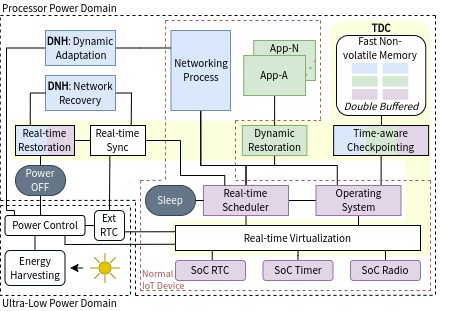
\includegraphics[width=0.6\linewidth]{chapters/Literature/diagram.jpg}
    \caption{FreeBie Architecture \cite{de2022Intermittently}.}
    \label{fig:freebie_paper_arch}
\end{figure}
\begin{figure}[t]
    \centering
    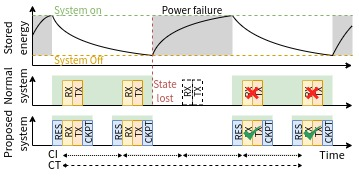
\includegraphics[width=0.6\linewidth]{chapters/Literature/intro.jpg}
    \caption{Intermittently-powered device operation. In a nonprotected system even a single power failure causes the network state to be lost, requiring unnecessary new handshakes. In our proposed system (FreeBie System) the network state is stored and restored to/from nonvolatile memory enabling to sustain connections. CI: connection interval, CT: connection timeout, RES: state restore, CKPT: state checkpoint, RX/TX: reception/transmission. region denotes the period of devices on time \cite{de2022Intermittently}.}
    \label{fig:freebie_paper_conn}
\end{figure}

In the realm of intermittent connectivity solutions, the FreeBie architecture emerges as a pivotal contender, offering a distinctive approach to achieving Bluetooth Low Energy (BLE) communication on intermittently-powered wireless devices \cite{de2022Intermittently}. This architecture, shown in Figure \ref{fig:freebie_paper_arch}, introduces an adaptive framework that tailors connection parameters according to the available harvested energy, facilitating efficient communication in resource-constrained environments. One of its significant features is to maintain BLE connections despite intermittent power, as illustrated in Figure \ref{fig:freebie_paper_conn}. Its unique ability to enable bi-directional communication and dynamically manage network connections fills a critical gap in the domain of intermittently-powered devices. Also it supports preemptive scheduling, allowing network processes to take precedence over application or operating system processes.
\vspace{1\baselineskip}

\noindent These components within FreeBie architecture serve a critical role on achieving the battery less operation:
\begin{itemize}
    \item \textbf{FRAM (Ferroelectric RAM):} FRAM is a non-volatile memory technology that offers high read/write speeds and low power consumption. It stores data and program code, ensuring persistence during power cycles. FRAM preserves memory sections during each checkpoint and stores context across separate allocated regions for OS processes, Network processes, and Application processes.
    
    \item \textbf{External RTC (Real-Time Clock):} The external RTC provides accurate timekeeping even during device power-off periods. This time reference is vital for synchronisation and event scheduling. The external RTC remains always powered through onboard capacitors and can control processor power domains using the Power switch and Power control module.
    
    \item \textbf{Time-Deterministic Checkpointing and Restore:} This component maintains data integrity by regularly capturing the device's state. In cases of power disruptions, the system can restore to a known state, preventing data loss and ensuring system consistency. It leverages External RTC and FRAM for uninterrupted atomic operations.
    
    \begin{itemize}
        \item \textit{Real-time RTC sync:} This subcomponent synchronises the Ext. RTC with the onboard RTC during each real-time operation resumption from power-off state. It uses FRAM to store the synchronising time \(T_{Sync}\) in the OS context.
        \item \textit{Real-time/Dynamic Restoration:} Upon resuming from power-off state, this component restores processes from FRAM for OS processes, network processes, and real-time application processes, as scheduled by the scheduler.
        \item \textit{Dynamic Handling of Network Connection:} Responsible for network recovery and dynamic network adaptation, this subcomponent ensures network recovery in unexpected power-offs and adapts to energy conditions while maintaining connection.
    \end{itemize}
    
    \item \textbf{Power Control:} Governing power state transitions, power control mechanisms by managing power-on timings, task execution, and low-power modes.
    
    \item \textbf{Super Capacitors and Energy Harvesters:} Integral to FreeBie's energy autonomy, super capacitors and energy harvesters contribute to storing and harnessing energy from ambient sources.
\end{itemize}

\noindent However, since the architecture relies on external components such as FRAM and an external RTC, it impacts factors like system cost, size, and energy consumption. To address this, the authors suggest future exploration into developing a FreeBie version that integrates next-generation System on Chip (SoC) technology and leverage more energy-efficient harvesters.
\vspace{1\baselineskip}

\noindent Furthermore, the FreeBie architecture is designed to support intermittently-powered end devices, but a notable research gap lies in the absence of support for intermittently-powered hosts on both sides of BLE communication. While the architecture excels in enabling communication between intermittently-powered device and continuously powered hosts, there's potential for innovation in extending its capabilities to encompass two intermittently-powered end nodes. This extension could unlock novel use cases in wireless sensor networks, broadening the applicability of the FreeBie architecture.

\section{Body Sensor Network}
The evolution of Body Sensor Networks (BSNs) has marked a significant milestone in healthcare and wellness monitoring. These networks, composed of wearable sensors, offer real-time data collection, analysis, and transmission, empowering individuals and healthcare professionals with valuable insights into physiological and medical conditions. BSNs have demonstrated remarkable potential in applications ranging from remote patient monitoring to sports performance analysis and beyond.
\vspace{1\baselineskip}

\noindent Early research in BSNs primarily focused on sensor integration and data aggregation techniques \cite{5678072}. These studies paved the way for more advanced BSNs capable of real-time health monitoring. The advent of wearable devices with integrated physiological sensors has led to the development of innovative solutions for continuous monitoring of vital signs such as heart rate, temperature, and electrocardiogram (ECG) signals \cite{BSNreview}, \cite{6555588}. These advancements enable early detection of anomalies and timely intervention in critical situations.
\vspace{1\baselineskip}

\noindent The energy requirements of BSNs vary based on the complexity of sensors and the data transmission frequency. Wearable sensors that capture high-resolution data, such as ECG signals, demand a continuous power source for accurate monitoring. However, battery limitations hinder the potential for uninterrupted data collection. This challenge becomes even more pronounced when considering the size and weight restrictions of wearable devices \cite{WANG2020112410}, \cite{4755157}, \cite{6755575}.
\vspace{1\baselineskip}

\noindent The integration of battery-free IoT devices within BSNs offers a promising solution to the energy challenge \cite{5370806}. This innovation not only extends the operational lifetime of BSNs but also opens the door to continuous and sustainable monitoring. Also it could be affordable (less than US\$2 each when manufactured in volume), disposable, small, and easy to use \cite{5370806}. Although there are already some Battery free Wireless BSN solutions but they do use near-field-enabled clothing capable of establishing wireless power and data connectivity between multiple distant points around the body to create a network of battery-free sensors interconnected by proximity to functional textile patterns.\cite{Lin_Kim_Achavananthadith_Kurt_Tan_Yao_Tee_Lee_Ho_2020}
\vspace{1\baselineskip}

\noindent In summary, the evolution of BSNs has been characterised by breakthroughs in sensor integration and wireless communication. However, the challenge of battery dependence has persisted. The emergence of battery-free IoT devices powered by energy harvesting techniques presents a transformative solution. As ongoing research continues to address energy challenges and optimise device performance, the future of BSNs holds the promise of continuous and sustainable healthcare monitoring.
\chapter{Architecture and System Design}
\label{chap:architecture}

This chapter aims to explore the architecture and design of the CardioSync framework, building upon the problem statement from Chapter 1 and with the aid of literature review in Chapter 2.

\noindent The central issue addressed in this thesis revolves around the existing FreeBie architecture, which grants intermittent power capabilities solely to one end device of a BLE network. To extend this to both end devices, the challenge lies in devising a synchronisation mechanism within a battery-free architecture and crafting an efficient wake-up scheduling strategy.

\noindent In response to these challenges, this chapter outline the architectural evolution from FreeBie to CardioSync, highlighting the transformative integration of the framework. Also this chapter, we provide a thorough analysis of the proposed architecture, focusing on key components, interactions, and overall design concepts.

\noindent Furthermore, to aid in understanding the conceptual landscape, \autoref{fig:architecture} illustrates the high-level architecture of the CardioSync framework within the existing FreeBie model.


\section{Overview of Existing FreeBie Model}
Before delving into the details of the CardioSync framework, it is essential to establish a foundation by understanding the existing FreeBie model. FreeBie, a notable advancement in the field of battery-less embedded systems, provides the groundwork, incorporating innovative energy harvesting techniques and intermittent operation strategies to enable devices to function without conventional batteries.  

\noindent From Figure \ref{fig:architecture}, it can be noted that the whole model of FreeBie is built on top of any normal IoT embedded systems architecture with BLE networking stack. FreeBie includes components like FRAM, External RTC, Time-Deterministic Checkpointing and Restore, and Power Control, all of which leverage the base system's real-time virtualization of time and peripherals to enable unobstructed communication on an intermittently-powered budget \cite{de2022Intermittently}.

\begin{figure}[H]
    \centering
    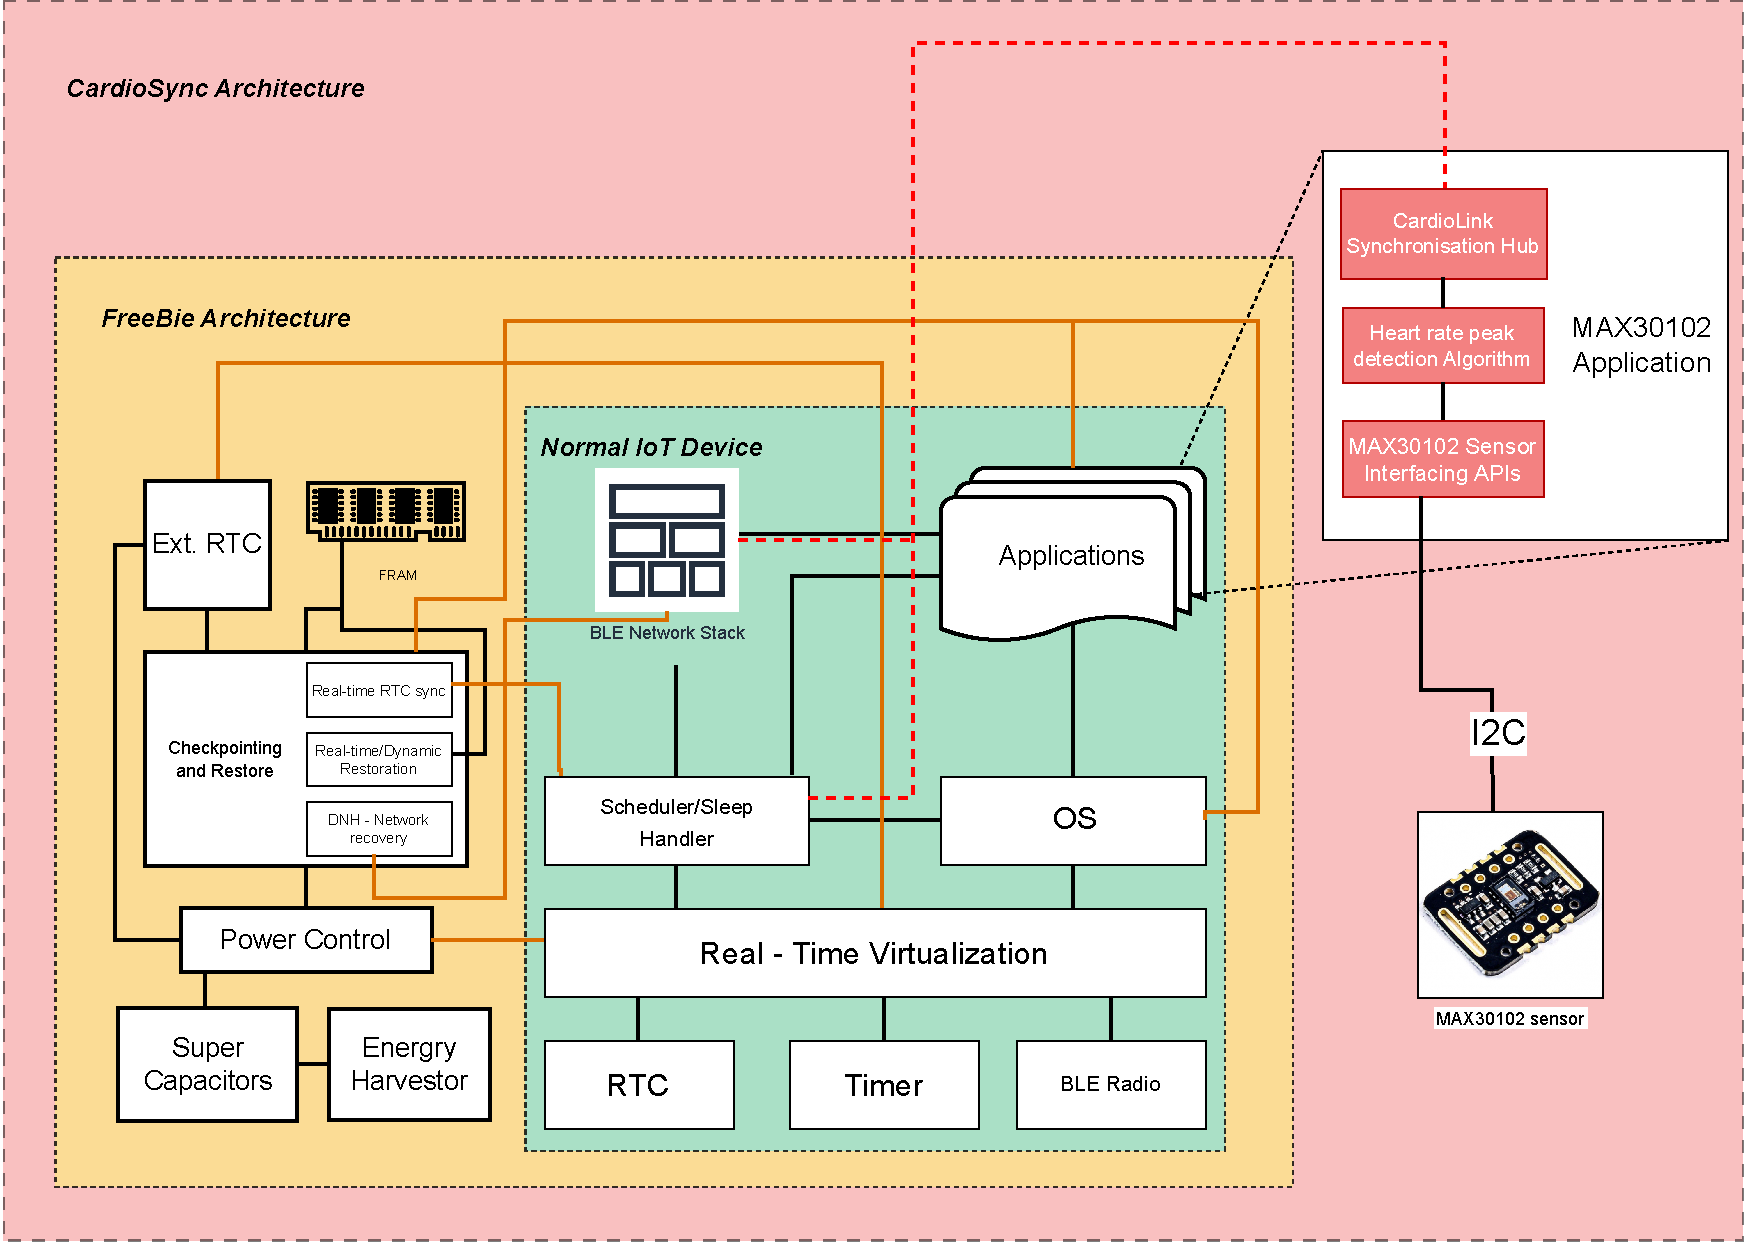
\includegraphics[width=\linewidth]{chapters/Architecture/architecture.pdf}
    \caption{High Level Architecture of the CardioSync framework}
    \label{fig:architecture}
\end{figure}

\noindent Each of these components serve a critical role on achieving the battery less operation:
\begin{itemize}
    \item \textbf{FRAM (Ferroelectric RAM):} FRAM is a non-volatile memory technology that offers high read/write speeds and low power consumption. It stores data and program code, ensuring persistence during power cycles. FRAM preserves memory sections during each checkpoint and stores context across separate allocated regions for OS processes, Network processes, and Application processes.
    
    \item \textbf{External RTC (Real-Time Clock):} The external RTC provides accurate timekeeping even during device power-off periods. This time reference is vital for synchronisation and event scheduling. The external RTC remains always powered through onboard capacitors and can control processor power domains using the Power switch and Power control module.
    
    \item \textbf{Time-Deterministic Checkpointing and Restore:} This component maintains data integrity by regularly capturing the device's state. In cases of power disruptions, the system can restore to a known state, preventing data loss and ensuring system consistency. It leverages External RTC and FRAM for uninterrupted atomic operations.
    
    \begin{itemize}
        \item \textit{Real-time RTC sync:} This subcomponent synchronises the Ext. RTC with the onboard RTC during each real-time operation resumption from power-off state. It uses FRAM to store the synchronising time \(T_{Sync}\) in the OS context.
        \item \textit{Real-time/Dynamic Restoration:} Upon resuming from power-off state, this component restores processes from FRAM for OS processes, network processes, and real-time application processes, as scheduled by the scheduler.
        \item \textit{Dynamic Handling of Network Connection:} Responsible for network recovery and dynamic network adaptation, this subcomponent ensures network recovery in unexpected power-offs and adapts to energy conditions while maintaining connection.
    \end{itemize}
    
    \item \textbf{Power Control:} Governing power state transitions, power control mechanisms by managing power-on timings, task execution, and low-power modes.
    
    \item \textbf{Super Capacitors and Energy Harvesters:} Integral to FreeBie's energy autonomy, super capacitors and energy harvesters contribute to storing and harnessing energy from ambient sources.
\end{itemize}

\noindent Leveraging these components, FreeBie achieves its ultimate objective of enabling seamless BLE communication and operation within an intermittently-powered paradigm \cite{de2022Intermittently}.

\section{Identification of Areas for Improvement}
While FreeBie represents a significant advancement in the realm of battery-less embedded systems, the intermittent power operation of devices within a communication network introduces specific challenges. These challenges are particularly pronounced when both end devices within the network operate on intermittent power sources. In response, significant areas for improvement have been identified, prompting the development of the CardioSync framework.

\noindent The key areas for improvement within the FreeBie model include:

\begin{itemize}
    \item \textbf{Bidirectional Intermittent Operation:} The original FreeBie architecture features asymmetric operation with periodic advertisement, where one end device intermittently operates while the other remains continuously powered. CardioSync should aim to extend energy efficiency to both end devices, enabling bidirectional intermittent operation.
    
    \item \textbf{Dynamic Wake-Up Scheduling:} Intermittent operation necessitates strategic wake-up scheduling to optimize BLE connection setup and minimize energy consumption. The complexity increases when both end devices experience intermittent power cycles. The architecture in design should aim to create an intelligent wake-up strategy that aligns with the dynamic power availability of intermittently-powered devices, ensuring synchronised connection setup.

\end{itemize}

\noindent By distinguishing these areas for improvement, the CardioSync framework aims to enable robust synchronisation between intermittently-powered devices, using external fixed common clock pulse. The figure \ref{fig:freebie_vs_cardiosync} highlights the difficulty encountered in establishing a connection between intermittent end devices using the FreeBie architecture. Additionally, it showcases the approach used by CardioSync to address this obstacle via the utilization of external pulse.

\begin{figure}[H]
    \centering
    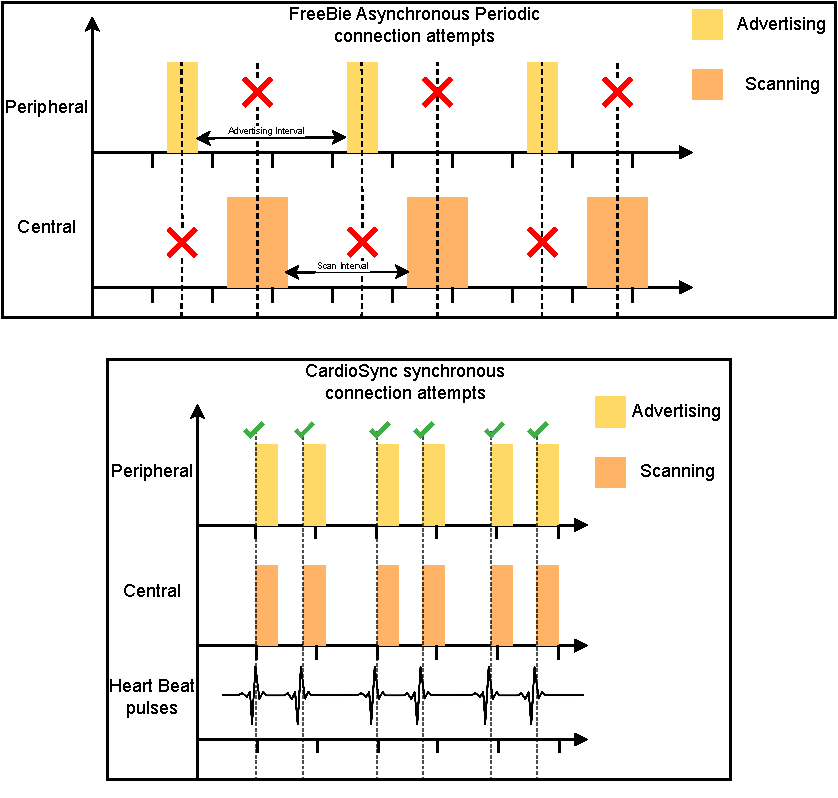
\includegraphics[width=0.6\linewidth]{chapters/Architecture/Freebie Vs. CardioSync.pdf}
    \caption{Conceptual diagram showing connection setup events of both end devices in FreeBie vs. CardioSync framework}
    \label{fig:freebie_vs_cardiosync}
\end{figure}

\section{Proposed Contribution - CardioSync Framework Integration}
The CardioSync framework represents a novel approach to address the synchronisation and connectivity challenges inherent in battery-less embedded systems. By integrating heart rate peak detection algorithm with Bluetooth Low Energy (BLE), CardioSync establishes synchronisation points and enhances connectivity even in the absence of continuous power.

\noindent The integration of the CardioSync framework is structured around the following key aspects:

\begin{itemize}
    \item \textbf{Heart Rate Peak Detection Algorithm:} CardioSync leverages advanced heart rate peak detection algorithms. These algorithms interpret heart rate data collected from the MAX30102 sensor interfaced with the MCU. The detection of heart rate peaks serves as the basis for scheduling synchronisation events, allowing intermittently-powered devices to synchronise their activities.
    
    \item \textbf{Synchronised BLE Connection:} In tandem with heart rate pulse detection, CardioSync synchronises BLE connection functionalities and enables the orchestrated scheduling of BLE advertising and scanning events that aligns with heart rate patterns, enhancing both connectivity and energy efficiency.
    
    \item \textbf{Establishing synchronisation Points:} The CardioSync framework introduces the concept of synchronisation points, which are strategically defined moments in time based on heart rate peaks. These points become the triggers for connection setup instances.
        
\end{itemize}

\noindent After a comprehensive review of available low-power heart rate detection sensors, the MAX30102 sensor from Maxim Integrated was selected as the heart rate monitor for the CardioSync framework. The MAX30102 sensor, consuming less than 1 mW and featuring low shutdown current around 0.7 \(\mu\)A, fits seamlessly with CardioSync's design goals.

\section{Architectural Changes and Components}
The CardioSync framework extends the FreeBie architecture to introduce a real-time application named MAX30102 application. This addition brings forth new components that contribute to the key aspects discussed:

\begin{itemize}
    \item \textbf{MAX30102 Sensor Interfacing APIs:} These APIs facilitate interaction between the MAX30102 sensor and the MCU using nRF5 SDK's TWI module to communicate through \(I^2C\) interface. They enable the collection of sensor data, forming the foundation for the heart rate peak detection algorithm.
    
    \item \textbf{Heart Rate Peak Detection Algorithm:} This algorithm processes the sensor data from the MAX30102 sensor and accurately detects heart rate peaks. The algorithm's outputs are pivotal in establishing synchronisation points and facilitating precise BLE adversting or scanning initiation instances.
    
    \item \textbf{CardioLink synchronisation Hub:} Serving as the central hub, this component handles the heart rate peaks processing, synchronisation points and BLE connection initiations. It ensures coordination between heart rate peak detection algorithm and scheduling of BLE advertising or scanning through existing FreeBie architecture's scheduler. This ensures synchronisation with sleep and wake-up intervals aligned with heart rate intervals instead of periodic advertisement or scan. This key component enables both end devices to be intermittent and still able to establish a BLE connection.
    
\end{itemize}

\section{High-Level Operation Flow}
The CardioSync framework operates through a systematic sequence of steps, integrating the heart rate peak detection algorithm with BLE stack as follows:

\begin{enumerate}
    \item \textbf{Sensor Data Acquisition:} The process begins with the acquisition of sensor data through dedicated APIs. The MAX30102 sensor reads the IR sensor values, capturing blood flow information. These values are temporarily stored in a buffer.
    
    \item \textbf{Heart Rate Peak Detection:} The sensor data is then fed into the heart rate peak detection algorithm. This algorithm discerns peaks indicative of heart rate activity from the provided data.
    
    \item \textbf{CardioLink Hub Verification:} Once a heart rate peak is detected, the CardioLink synchronisation Hub steps in. It verifies whether the peak corresponds to a new occurrence. This verification is based on the PalRTCTicks linked with each peak.
    
    \item \textbf{Instant Advertisement/Scanning Scheduling:} When a verified heart rate peak is detected, the CardioLink Hub orchestrates instantaneous scheduling of BLE advertising or scanning events. This scheduling leverages the FreeBie architecture, enabling connection instances aligned with heart rate intervals.
    
    \item \textbf{Heart Rate Interval Calculation:} The CardioSync framework calculates the heart rate interval based on the timing of multiple detected heart rate peaks. This interval defines the temporal spacing between synchronisation points.
    
    \item \textbf{Sensor Data Collection Pause:} Upon calculating the heart rate interval using multiple peaks, the sensor data collection process is temporarily paused. This pause ensures accurate synchronisation and prevents unnecessary data acquisition.
    
    \item \textbf{synchronisation Point Establishment:} Using the calculated heart rate interval, synchronisation points are established. These synchronisation points serve as triggers for possible connection establishment instances between intermittently-powered devices.
    
    \item \textbf{Scheduled Advertisement/Scanning:} With synchronisation points in place, the CardioLink Hub schedules BLE advertising or scanning events within the heart rate interval. This ensures connectivity aligned with the heart rate patterns.
    
    \item \textbf{Iteration and Adaptation:} The process continues to iterate, adapting to the dynamic heart rate patterns and power availability till the connection setup is complete. The framework ensures synchronisation, connectivity even in intermittent power scenarios.
\end{enumerate}

\noindent The workings of the algorithm and the CardioSync framework will be elaborated upon in the upcoming Implementation chapter, providing a comprehensive understanding of the operational intricacies.

\chapter{Technical Implementation}
This chapter delves into the practical realization of the CardioSync framework, translating the architectural concepts and design discussed in the previous chapters into tangible code and functional components. This chapter aims to offer an in-depth explanation of the coding process, including flowcharts and pseudo-code representations, showcasing how the theoretical foundation transforms into a working system.

\section{Hardware and Software Setup}
The implementation of the CardioSync framework involves both hardware and software components. This section outlines the necessary hardware setup and software environment required for the realization of the framework.

\subsection{Hardware Setup}
The CardioSync framework is built upon the FreeBie model, integrating the MAX30102 sensor. The hardware setup comprises the following components:

\begin{itemize}
    \item \textbf{FreeBie Mote:} This custom board in \autoref{fig:freebie} incorporates essential components, including the nRF52840 ARM-Based MCU module (\textit{EYSKBNZWB}) with BLE radio support, the External RTC and power management module (\textit{AB1815}), and FRAM (\textit{MB85RS4MT}). These components provide the foundation for the framework's intermittent operation.
    
    \item \textbf{MAX30102 Sensor Board:} The MAX30102 sensor board from Maxim Integrated serves as a critical element for heart rate monitoring. The sensor board features built-in pull-up resistors of 4.7k\(\Omega\) in the \(I^2C\) pin outs. However, for our specific use case, these resistors were not used, as the on-board pull up resistors of the nRF52840 were employed instead through Software configuration.
    
    \item \textbf{Connection Configuration:} Based on the pinout configuration of the FreeBie schematics, GPIO pin P0.04 is connected to the SCL (Serial Clock Line) of the MAX30102, while GPIO pin P0.27 is connected to the SDA (Serial Data Line). The MAX30102 is powered by the onboard super capacitors, connected to the \(V_{Batt}\) pinout of the FreeBie Mote.
\end{itemize}


\begin{figure}[H]
    \centering
    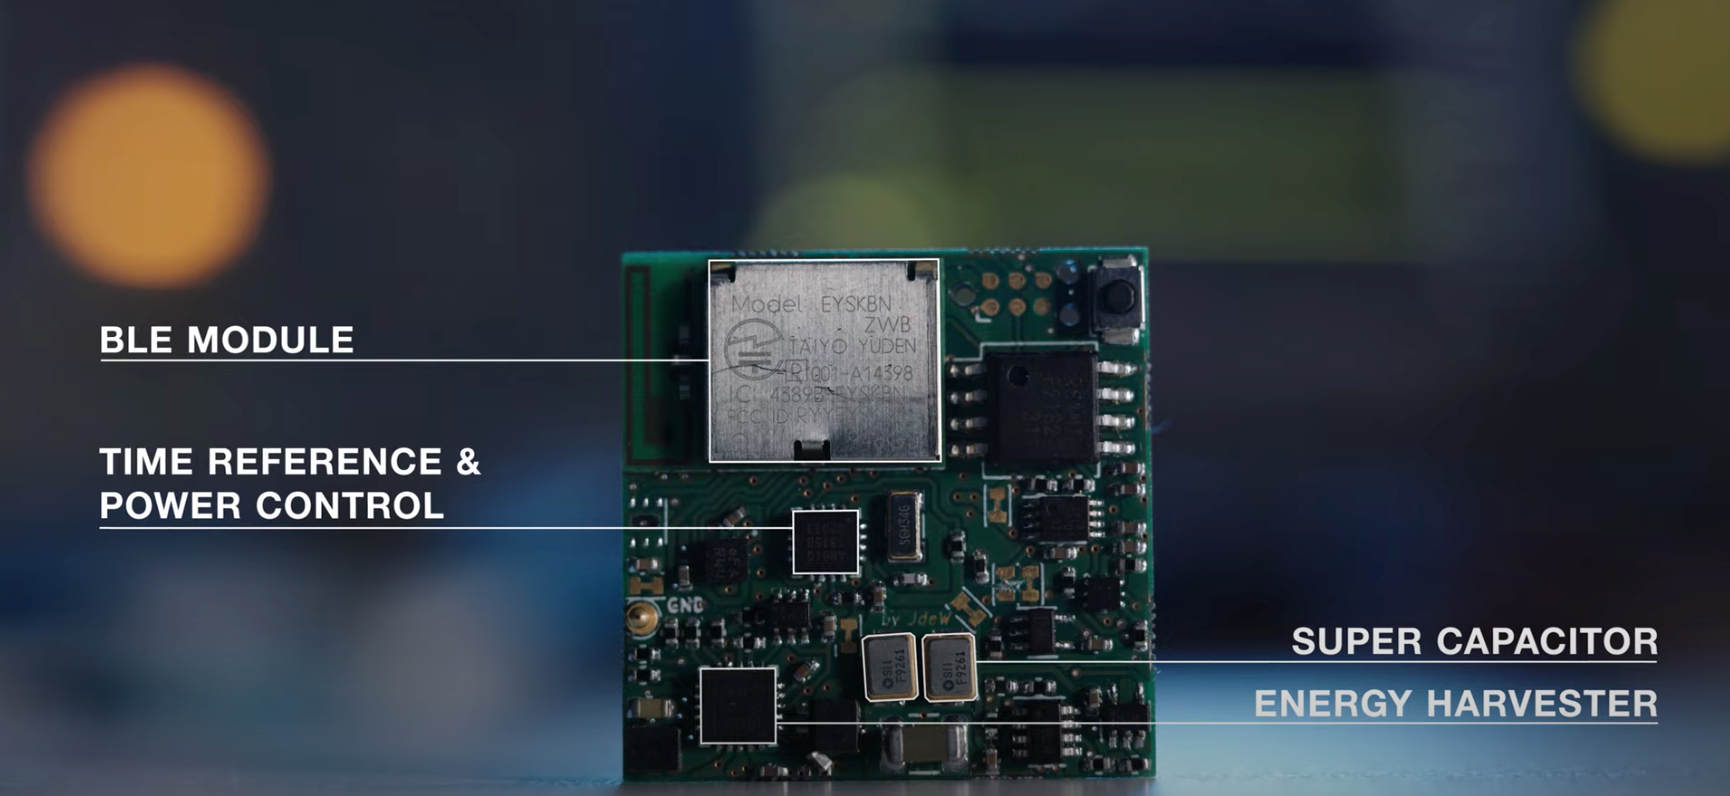
\includegraphics[width=\linewidth]{chapters/Implementation/Freebie.png}
    \caption{FreeBie Mote}
    \label{fig:freebie}
\end{figure}

\subsection{Software Setup}
\label{sec:software_setup_impl}

The implementation of the CardioSync framework builds upon the open-source FreeBie source code, available from the TUDelft Sustainable Systems Lab repository. The adaptation process involves customizing the existing \textit{"template"} application to accommodate the CardioSync system architecture  - MAX30102 sensor and the Heart Rate peak detection algorithm.

\subsubsection{Software Foundation and Customisation}

The entire FreeBie source code relies on the PacketCraft BLE stack, which seamlessly integrates nRF5 SDK libraries for driver interfaces and peripheral interactions. The code is specifically tailored for the nRF52840 MCU, utilizing the GNU ARM Embedded ToolChain, thus eliminating the need for additional build support or toolchain.

\subsubsection{MAX30102 Sensor Interfacing}

For interfacing with the MAX30102 sensor, nRFx driver for the Two Wire Interface - Master (TWIM) is employed. This involves enabling the necessary configurations in the \textit{sdk\_config.h} file to activate the TWIM in the system. Subsequently, relevant APIs provided by the nRFx library are utilized for reading from and writing to the \(I^2C\) interface.
 
\subsubsection{BLE Stack Configuration}

In the context of the BLE stack, PacketCraft's CMake configurations take charge of initializing the MCU as either a Peripheral or Central device. Two specific CMake definitions, namely \texttt{INIT\_PERIPHERAL} and \texttt{INIT\_CENTRAL}, determine the operational mode. PacketCraft then leverages essential components like the \textit{Device Manager (DM) and the Application framework main module (App)} to initialize the BLE stack. This equips the framework with APIs that helps with the initiation and termination of advertising or scanning activities depending on whether the device is operating as a Peripheral or Central.

\subsubsection{Timing and Scheduling}

Both the FreeBie and CardioSync frameworks require precise timing and scheduling mechanisms. PacketCraft's Wireless Software Foundation (WSF) OS layer offers essential APIs for managing the AppTimer functionality. These APIs enable the start and stop of timers, ensuring accurate timing operations necessary for the effective functioning of both frameworks.


\section{MAX30102 Sensor Interfacing}
Integral to the CardioSync framework is the seamless integration and interfacing with the MAX30102 sensor via the \(I^2C\) interface. This section delves into the practical implementation and methodologies used, outlining the steps taken to interface the MAX30102 sensor with the FreeBie architecture effectively.

\noindent As outlined in the previous section (\autoref{sec:software_setup_impl}), the existing "template" application within the FreeBie source code is extended to incorporate the MAX30102 sensor functionality. This is achieved by introducing a new source file named "\texttt{MAX30102\_main.c}", which houses all the necessary functions, declarations, and configurations essential for successful sensor interfacing and data acquisition.

\noindent The interfacing with the MAX30102 sensor involves several key functions, including sensor initialization, configuration setup, and data acquisition. Here is an in-depth look at these steps:

\subsection{Sensor Initialization and Configuration}
\label{sec:sensor_config}
The initialization of the MAX30102 sensor involves configuring its various registers to ensure optimal performance while minimizing power consumption. To achieve this, the \texttt{MAX30102\_init()} function is implemented. Within this function, several critical registers are configured as follows:

\begin{itemize}
    \item \textbf{REG\_INTR\_ENABLE\_1 (0x02U):} This register is set with the value 0xC0 to enable the "A\_FULL\_EN" interrupt, which triggers when the FIFO is full and data is ready for reading.
    
    \item \textbf{REG\_FIFO\_CONFIG (0x08U):} The FIFO configuration register is set with settings such as averaging 4 samples per entry, setting FIFO size to 32 (which triggers Interrupt 1 when full), and disabling FIFO rollover.
    
    \item \textbf{REG\_MODE\_CONFIG (0x09U):} Configures the operational mode of the sensor. In the context of CardioSync, heart rate mode is selected while disabling Spo2 measurements.
    
    \item \textbf{REG\_SPO2\_CONFIG (0x0AU):} Sets parameters for data acquisition including a sampling rate of 50 samples per second, ADC range of 4096nA, pulse width of 118us, and 16-bit ADC resolution.
    
    \item \textbf{REG\_LED1\_PA(0x0CU), REG\_LED2\_PA (0x0DU):} Configures LED current; for CardioSync, 1mA is set for both LED1 and LED2.
\end{itemize}

\noindent By meticulously configuring these registers, the MAX30102 sensor is primed to operate within desired parameters and less power consumption, yet capturing accurate blood flow data for heart rate analysis.

\subsection{Data Acquisition}
\label{sec:sensor_data_impl}
The data acquisition element of the MAX30102 sensor interfacing facilitates the collection of relevant sensor data to identify heart rate peaks. This section outlines the methodology employed for data collection, buffering, and sliding window management within the CardioSync framework.

\noindent A two dimensional buffer of a maximum capacity of 2 x 500 entries is employed to store the current sensor values and their respective RTC ticks at which they are read. These values are continuously read from the MAX30102 sensor's FIFO and \texttt{PalRtcCounterGet()} at a predetermined sampling rate. In parallel, a sliding window of size 10 is established, ensuring that the latest 10 sensor values are always maintained within the window.

\noindent The data acquisition process is orchestrated by the following key steps:

\subsubsection{WSF Timer Initialization}
Upon successful sensor initialization, a WSF timer named "\texttt{MAX30102Timer}" is initiated. The timer's period is determined by \(1000\) divided by the chosen sampling rate. In the context of the CardioSync architecture, a sampling rate of \(100\) Hz is selected after rigorous evaluation of both the sensor's capabilities and the heart rate peak detection algorithm. Further insights into the rationale behind this decision are provided in the upcoming "Results" chapter (\ref{chap:results}).

\subsubsection{FIFO Read and Buffering}
When the "\texttt{MAX30102Timer}" timer expires, it triggers an event labeled "MAX30102\_TIMER\_IND." Within the scope of this event, the MAX30102 sensor's FIFO is read using the "\texttt{MAX30102\_read\_fifo()}" function. This function relies on the \texttt{nrfx\_twim} module to extract the current IR and Red LED values from the FIFO. Among these values, the IR value holds samples for heart rate peak detection. Consequently, the IR value is paired with the corresponding RTC ticks recorded during the sensor read and appended to the end of the buffer.

\subsubsection{Continuous Data Acquisition}
Following the FIFO read and buffering, the "\texttt{MAX30102Timer}" is restarted. This sequence of operations repeats at intervals of \(10\) ms until the sliding window, positioned at the end of the buffer, is completely populated with the latest \(10\) values. This data acquisition process ensures that the sliding window is consistently updated, offering a continuous stream of data for subsequent heart rate peak detection.

\subsubsection{Heart Rate Peak Detection}
The sensor values contained within the sliding window are then subjected to the heart rate peak detection algorithm only if the average of those 10 values in Sliding window more than 8000. Peak detection is conducted only when the sensor comes into contact with a person. In the absence of such contact, the average value is expected to be below 8000. This algorithm is designed to identify peaks indicative of heart rate activity, allowing the CardioSync framework to accurately determine heart rate patterns based on the IR values.

\noindent The iterative nature of this process guarantees the availability of up-to-date sensor data for real-time heart rate analysis, ensuring the responsiveness and accuracy of the CardioSync system.

\subsubsection{Pseudocode Representation}
For better understanding, here is a pseudocode representation of the data acquisition process:

\begin{algorithm}[H]
\caption{MAX30102 Sensor Data Acquisition}
\begin{algorithmic}[1]

\State Initialize 2D Buffer with maximum capacity of 2 x 500
\State Initialize Sliding Window size as 10
\State Initialize "\textit{\texttt{MAX30102Timer}}" with period \(1000 / Sampling\ Rate\)
\State Start "\textit{\texttt{MAX30102Timer}}"

\State Wait for "\textit{\texttt{MAX30102Timer}}" to expire
\If{\textit{\texttt{MAX30102Timer}} expired}
    \State Read MAX30102 sensor's FIFO using "MAX30102\_read\_fifo()"
    \State Append IR value and corresponding RTC ticks to Buffer
    \If{Sliding Window is full and Average > 8000}
        \State Perform Heart Rate Peak Detection on Sliding Window data
    \EndIf
    \State Restart "\textit{\texttt{MAX30102Timer}}"
\EndIf

\end{algorithmic}
\end{algorithm}

\subsection{Heart Rate Peak Detection Algorithm}
\label{sec:heart_rate_algo_impl}
Initially, an attempt was made to utilize Maxim Integrated's heart rate peak detection algorithm developed for MAXREFDES117. This algorithm employed a method of peak identification by calculating a fixed threshold and detecting peaks above that threshold. Additionally, it employed a fixed threshold for removing closely spaced peaks based on a parameter \(n_{min\_distance}\). However, this approach proved ineffective for the CardioSync framework due to the dynamic and varying nature of the continuous sensor data readings obtained from the MAX30102. As shown in Figure~\ref{fig:dynamic_threshold}, the sensor data exhibited fluctuations that necessitated a more adaptive and dynamic thresholding approach.

\begin{figure}[H]
    \centering
    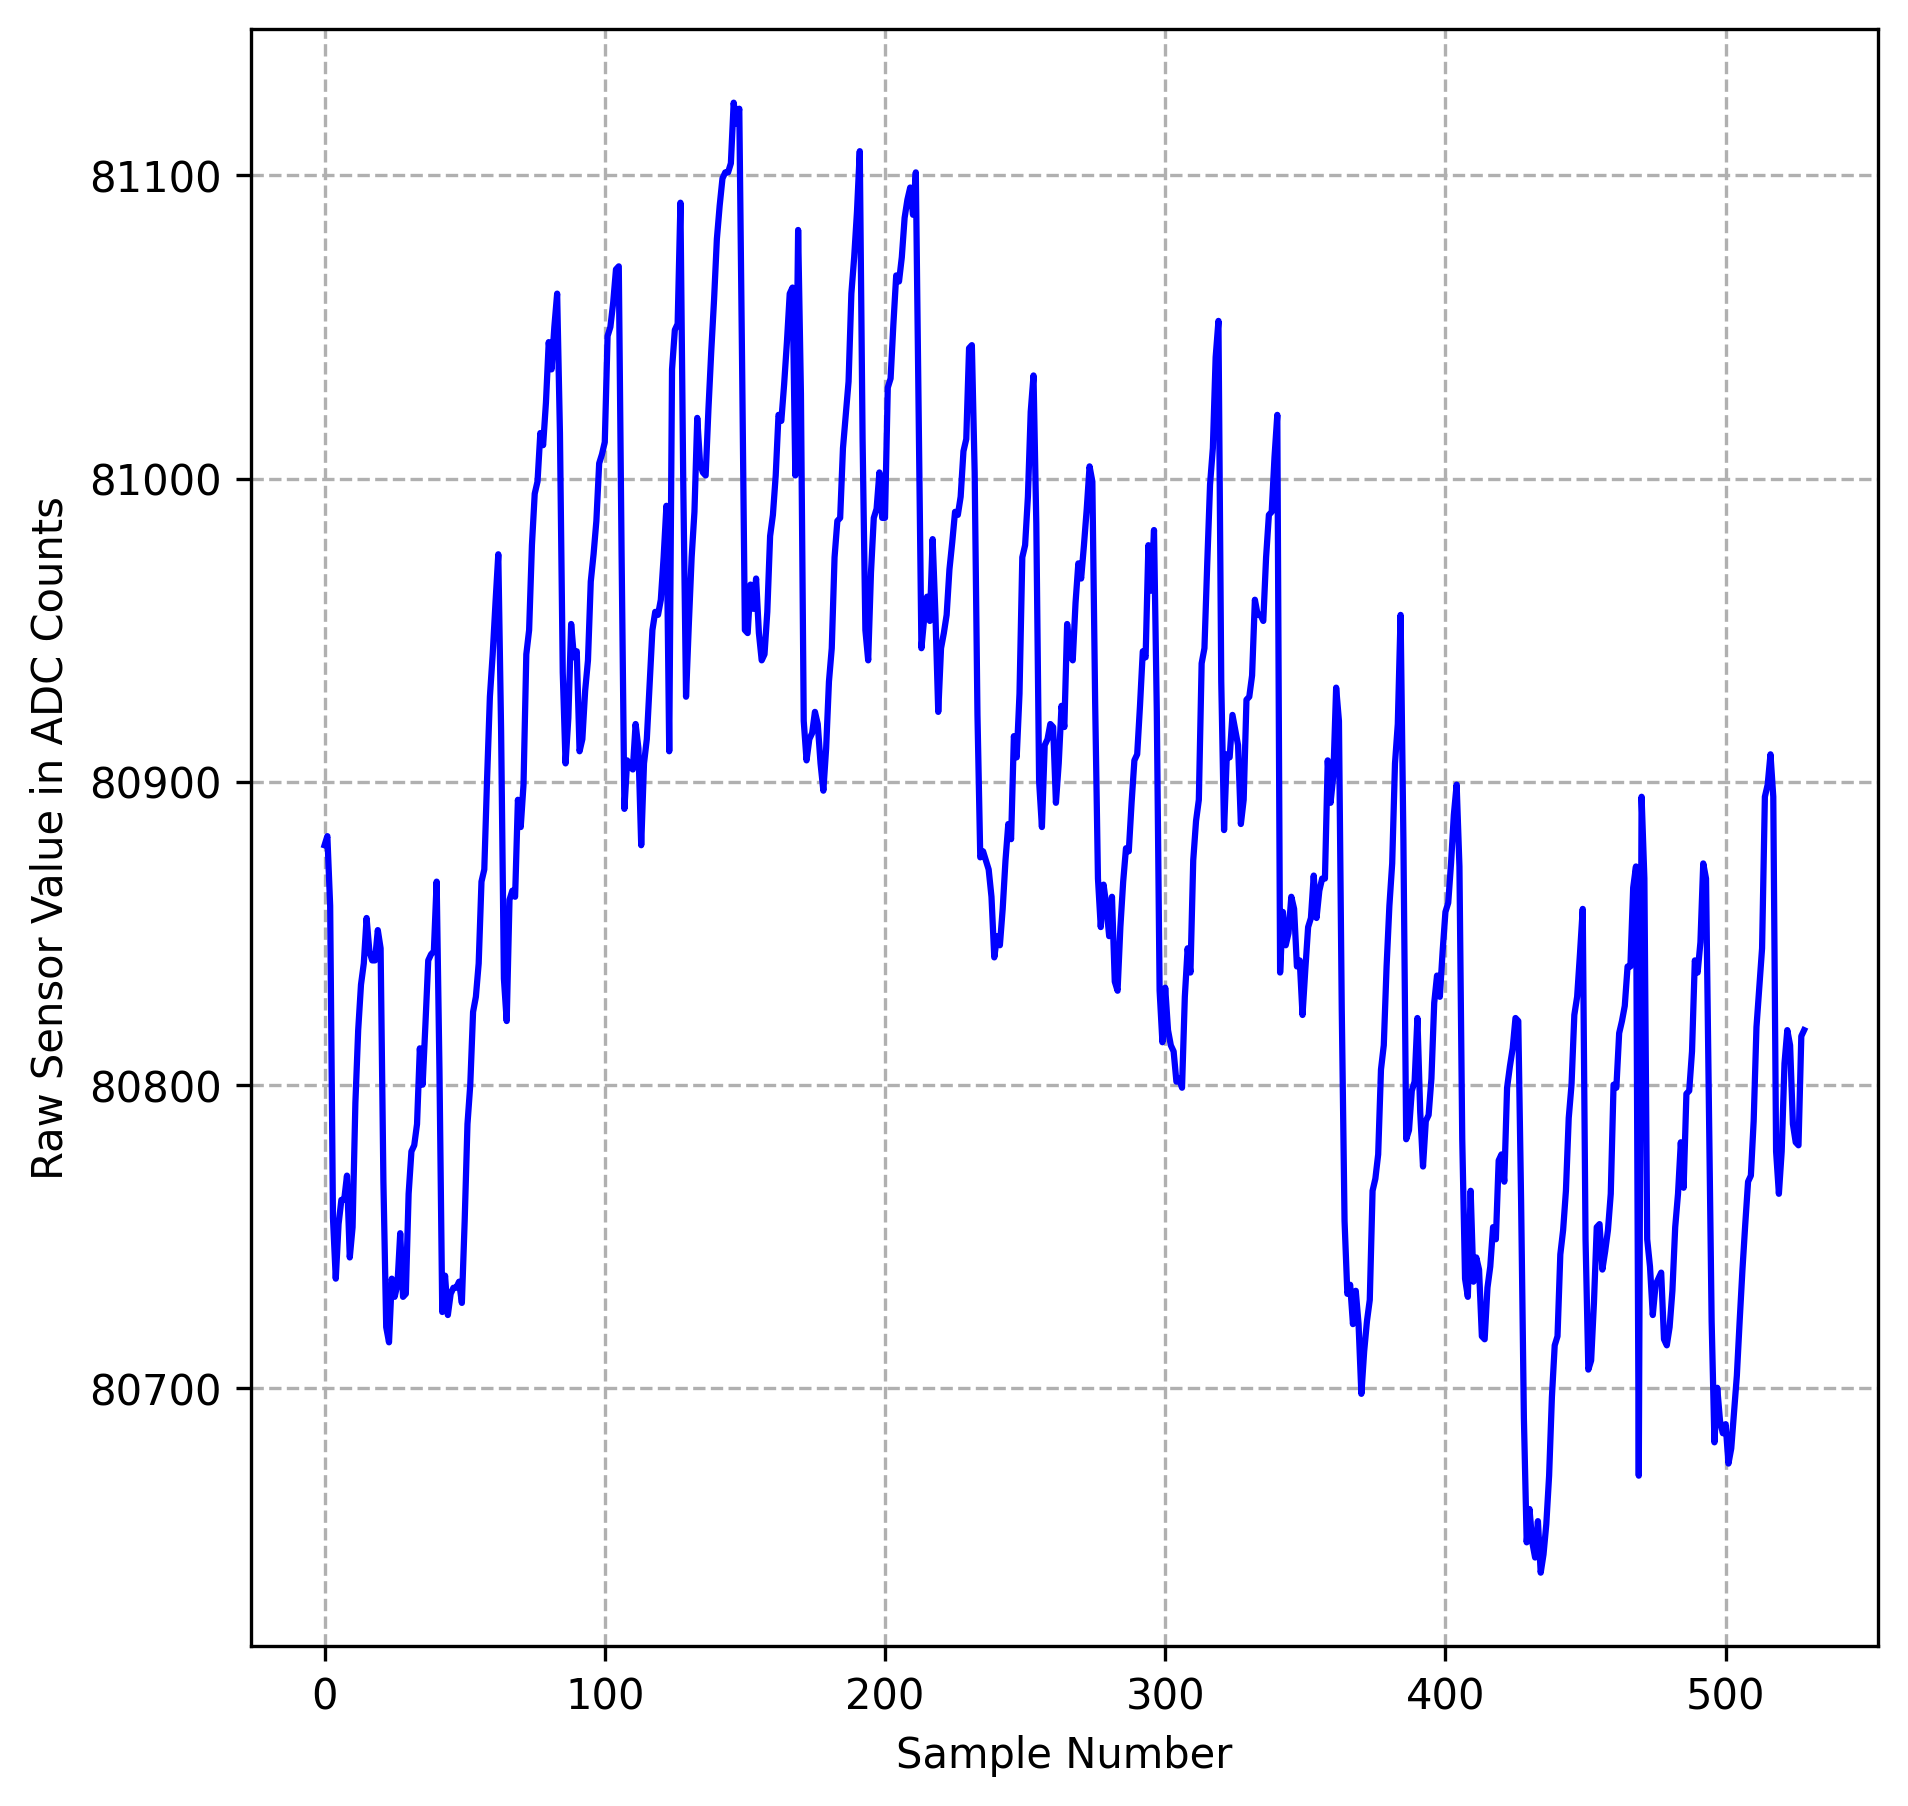
\includegraphics[width=0.7\linewidth]{chapters/Implementation/dynamic_threshold.png}
    \caption{Dynamic and fluctuating nature of continuous sensor data readings from MAX30102}
    \label{fig:dynamic_threshold}
\end{figure}

\noindent In light of these challenges, the decision was made to adopt an alternative approach that leverages the derivatives of the sensor data for peak detection. This approach was more suitable for handling the varying nature of the sensor readings and provided a robust means of detecting heart rate peaks.

\noindent The heart rate peak detection algorithm using derivatives operates as follows:

\begin{enumerate}
    \item \textbf{Data Preprocessing:} The raw sensor data collected from Sliding window buffer, denoted as \(a_{ir}\), undergoes preprocessing steps. The algorithm removes the DC component by calculating the mean and subtracting it from the data. This step is essential to eliminate any static offset and focus on the variations caused by heartbeats.
    
    \item \textbf{Moving Average:} The \(a_{ir}\) data is then updated using a moving average of two neighboring samples on either side of each sample. This smoothing technique helps reduce noise and sharp variations in the data, facilitating more accurate peak detection.
    
    \item \textbf{Derivative Calculation:} The first derivative of the \(a_{ir}\) data, referred to as \(a_{ir\_diff}\), is calculated. This derivative provides insights into the rate of change of the signal, which is particularly useful for identifying rapid transitions characteristic of heart rate peaks.
    
    \item \textbf{Peak and Valley Detection:} The algorithm identifies peaks and valleys within the \(a_{ir\_diff}\) data. Peaks correspond to points where the derivative changes from positive to negative, indicating a downward slope. Valleys, conversely, represent points where the derivative changes from negative to positive, indicating an upward slope. These points mark significant variations in the signal, which are indicative of heart rate peaks.
    
    \item \textbf{Peak Validation and Removal:} Detected peaks that are in close proximity to valley indices are discarded. A maximum distance threshold \(n_{valley\_distance}\) of value \textbf{4} is used to determine this proximity. Similarly, peaks that are too close to each other, within a distance threshold \(n_{peak\_distance}\) of value \textbf{15}, are also removed. These additional validation steps help ensure that the detected peaks correspond to distinct heart rate events.
    
    \item \textbf{Result Generation:} The algorithm generates a list of validated peak indices that represent heart rate peaks which likely to have occurred.
    
    \item \textbf{Callback and Post Processing:} For each detected and validated peak index, the algorithm invokes the \texttt{sensor\_callback} function. This function handles further processing, synchronization, and scheduling tasks related to the CardioSync framework.
\end{enumerate}

\noindent The constants \(n_{valley\_distance}\), and \(n_{peak\_distance}\) are empirically determined based on the characteristics of the sensor data and the expected heart rate patterns. These values ensure the reliability and accuracy of the peak detection process.

\noindent The algorithm's pseudocode is as follows:

\begin{algorithm}[H]
\caption{Heart Rate Peak Detection Algorithm - calculate\_heart\_rate}
\begin{algorithmic}[1]
\Function{calculate\_heart\_rate}{$a\_ir, callback$}
    \State Initialize arrays $a\_ir\_clean$, $a\_ir\_diff$, $peak\_indices$, and $valley\_indices$
    \State Calculate the mean of the raw IR sensor data $a\_ir$ to remove the DC component and obtain a centered signal
    
    \For{each data point $x$ in $a\_ir$}
        \State Subtract the mean from each data point to center the signal around zero, storing the result in $a\_ir\_clean$
    \EndFor
    
    \For{each data point $x$ in $a\_ir\_clean$}
        \State Apply a moving average filter to $a\_ir\_clean$ by averaging nearby two data points on both side to reduce noise and fluctuations
    \EndFor
    
    \For{each data point $x$ in $a\_ir\_clean$}
        \State Calculate the first derivative of the filtered signal $a\_ir\_clean$ to highlight changes in the signal, storing the result in $a\_ir\_diff$
    \EndFor

    \For{each index $x$ in the range from $1$ to $n - 2$, where $n$ is the length of $a\_ir\_diff$}
        \If{$a\_ir\_diff[x - 1]$ is positive \textbf{and} $a\_ir\_diff[x]$ is negative}
            \State Store the peak index $x$ in the $peak\_indices$ array
        \EndIf
    \EndFor

    \For{each index $x$ in the range from $1$ to $n - 2$, where $n$ is the length of $a\_ir\_diff$}
        \If{$a\_ir\_diff[x - 1]$ is negative \textbf{and} $a\_ir\_diff[x]$ is positive}
            \State Store the peak index $x$ in the $valley\_indices$ array
        \EndIf
    \EndFor
    
    \State Apply a post-processing step to remove peaks that are too close to each other using $n\_peak\_distance$
    % \For{each index $i$ in the range from $0$ to $peak\_indices\_length - 2$}
    %     \If{$peak\_indices[i + 1] - peak\_indices[i] < n\_peak\_distance$}
    %         \State Remove the peak at index $i + 1$ from $peak\_indices$
    %     \EndIf
    % \EndFor
    
    \State Apply a post-processing step to remove peaks that are close to valley indices using $n\_valley\_distance$
    % \For{each peak index $p$ in $peak\_indices$}
    %     \For{each valley index $v$ in $valley\_indices$}
    %         \If{$|p - v| < n\_valley\_distance$}
    %             \State Remove the peak at index $p$ from $peak\_indices$
    %         \EndIf
    %     \EndFor
    % \EndFor
    
    \State Call the callback function with the detected peak indices in $peak\_indices$
    
\EndFunction
\end{algorithmic}
\end{algorithm}

\noindent This algorithm's robustness and adaptability are crucial for accurately identifying heart rate peaks in the CardioSync framework, even when dealing with dynamic and fluctuating sensor data.

\section{Putting it Together}
With the fundamental components of the CardioSync framework established—ranging from hardware setup to heart rate peak detection algorithms, the next step involves integrating these elements into the FreeBie architecture. This section provides insight into how these various parts work together to create a functional system, ensuring accurate heart rate peak detection and synchronized BLE connection setup within a battery less system architecture.

\subsection{Framework Integration in the Template Application}
As previously mentioned in section \ref{sec:software_setup_impl}, the CardioSync framework is a part of the "\textit{template}" application in the FreeBie source code. Focusing from the start of execution, the MAX30102 sensor module is initialised through \texttt{MAX30102HandlerInit()} from within the application's stack init along with several required setup for BLE stack such as the \textit{Device Manager} and \textit{Application Manager}, \textit{Slave or Master initialization} according to the device's operational mode.

\noindent Within the \texttt{MAX30102HandlerInit()} function, \texttt{MAX30102\_config() and MAX30102\_init()} performs the configuration and activation of the TWIM interface for the MAX30102 sensor with  the parameters and operating configurations discussed in Section \ref{sec:sensor_config}. It's noteworthy that the MAX30102 is assigned to \textit{TWI instance 1}, as \textit{TWI instance 0} is exclusively allocated for SPI communication with the external FRAM module in the FreeBie architecture.

\subsection{WSF Timer Setup and Template Application Start}
The MAX30102HandlerInit function also initialises vital WSF timers \textit{MAX30102Timer} and \textit{MAX30102RestartTimer}. The comprehensive roles and functionalities of these timers will be elaborated upon in the subsequent sections. 

\noindent Upon the successful initiation of the system's BLE stack and the MAX30102 sensor, the "template" application commences its operation by invoking \texttt{TemplateStart()}. This phase encompasses the registration of BLE-related callbacks and attribute server setups. This sequence ends with a trigger of a Device Manager reset, setting the stage for subsequent phases.

\subsection{Sensor Data Acquisition and Peak Detection}
With the Device Manager reset, all essential initializations have been accomplished, paving the way for sensor data acquisition with the invocation of the \texttt{MAX30102Start()} function within the context of the "\texttt{DM\_RESET\_CMPL\_IND}" event handler in \texttt{TemplateHandler()}. It triggers buffer clearance and sliding window initialization. Followed by that, it starts the primary \textit{MAX30102Timer}, which orchestrates sensor data reading at a 100Hz sampling rate and facilitates heart rate peak detection. The details of these processes are elaborated in Sections \ref{sec:sensor_data_impl} and \ref{sec:heart_rate_algo_impl}.

\subsection{Heart Rate Peaks Post Processing and BLE Connection Initiation}
With the successful identification of heart rate peaks, their corresponding indices within sliding window are passed to the \texttt{sensor\_callback()} routine, marking the commencement of post-processing and synchronization tasks. This pivotal mechanism forms the CardioLink Synchronisation hub component embedded within the CardioSync framework architecture.

\noindent For each heart rate peak, the concomitant system RTC tick is retrieved from the data stored in a two-dimensional buffer using its indices.This paired data allows the \texttt{sensor\_callback()} function to distinguish between new peaks and peaks that linger within the rotating buffer. When a new peak is identified, the function updates the global variable \texttt{average\_time\_diff}, encapsulating the average time difference between the present peak and the previously detected peaks, i.e., heart rate interval. This value plays a pivotal role in establishing heart rate-based synchronization points.

\subsection{BLE Connection Setup and Synchronization}
Subsequently, based on the system's operational mode, either advertisement or scan initiation happens using PacketCraft's Application Manager API, such as \texttt{AppAdvStart()} or \texttt{AppScanStart()}. These operations are executed utilizing carefully optimized BLE parameters, encompassing advertising interval, scanning interval, scan duration, and scan window. These parameters are strategically chosen based on the comprehensive evaluation of algorithm performance and system behavior outlined in the forthcoming Results and Evaluation(\autoref{chap:results}) under the table \ref{tab:ble_params}. 

\noindent This phase operates simultaneously with active sensor read at a 100Hz sampling rate and synchronized advertising or scanning events correlated to each detected heart rate peak.

\subsection{Adaptive Heart Rate Recalculation and System Power Management}
Following the detection of three peaks (\texttt{MAX\_PEAKS}), \texttt{MAX30102Stop()} is invoked, shutting down the sensor by configuring the \texttt{REG\_MODE\_CONFIG} register (0x09U) with the value 0x80. This activates the MAX30102 Shutdown Control bit, facilitating power-saving mode in sensor. Simultaneously, the \texttt{MAX30102Timer} is terminated, suspending active sensor read.

\noindent After this phase, BLE parameters are dynamically adjusted during runtime to ensure the scheduling of advertisement or scanning events aligned with the heart rate interval. This adjustment relies on the \texttt{average\_time\_diff} global variable, which is continously updated during active sensor read and heart rate peak detection. The modified BLE parameters are outlined in Table \ref{tab:modified_ble_params}.

\begin{table}[H]
\centering
\begin{tabular}{|cc|}
\hline
\multicolumn{2}{|c|}{\textbf{\begin{tabular}[c]{@{}c@{}}BLE Advertisement Parameters\\ (Peripheral)\end{tabular}}} \\ \hline
\multicolumn{1}{|c|}{\textit{Advertising Interval}} & Heart rate interval \\ \hline
\multicolumn{1}{|c|}{\textit{Advertising Duration}} & 10 seconds          \\ \hline
\multicolumn{2}{|c|}{\textbf{\begin{tabular}[c]{@{}c@{}}BLE Scan Parameters\\ (Central)\end{tabular}}}             \\ \hline
\multicolumn{1}{|c|}{\textit{Scan Interval}}        & Heart rate interval \\ \hline
\multicolumn{1}{|c|}{\textit{Scan Window}}          & 100 milliseconds    \\ \hline
\multicolumn{1}{|c|}{\textit{Scan Duration}}        & 10 seconds          \\ \hline
\end{tabular}
\caption{Modified BLE parameters during runtime based on calculated heart rate interval (\texttt{average\_time\_diff})}
\label{tab:modified_ble_params}
\end{table}

\noindent This sets the stage for real-time task scheduling through APIs like \texttt{AppAdvStart()} or \texttt{AppScanStart()} using modified BLE parameters, engaging the Checkpointing and Restore module embedded within the FreeBie architecture. It detects for inactivity in the system, here in our case it is caused by no active sensor reads, and then initiates the process that checkpoints the current state of system and proceeds to power down the microcontroller unit (MCU), thereby placing it into a sleep mode. The system resumes and restores its operations only during planned BLE connection events, then returning to a sleep state until the subsequent heart rate interval. The current phase of the BLE connection setup process relies on the synchronization point established through the heart rate interval. It aims to conserve power by adhering to the principles of the FreeBie architecture. This approach enables synchronized advertisement or scanning, as opposed to periodic asynchronous methods, in order to establish a connection between two battery-less endpoints. 

\noindent In cases where connection establishment eludes success even during this phase, the continuity of heart rate interval (\texttt{average\_time\_diff} may be compromised. Thus, an adaptive approach comes into play. To address this, the \texttt{MAX30102RestartTimer} set for a 10-second duration, is activated in tandem with the scheduled BLE connection synchronization points when the \texttt{MAX\_PEAKS} has been detected. Upon the timer expiry, the sensor data buffers, previously detected peaks, and the \texttt{average\_time\_diff} global variable are reset. Subsequently, \texttt{MAX30102Start()} is invoked anew, reinitiating active sensor read. This iterative process continues until successful BLE connection is established. Upon connection close, \texttt{MAX30102Start()} is re-invoked, initiating the entire process afresh.


\noindent In summary, the implementation of the CardioSync framework within the FreeBie architecture constitutes a cohesive integration of hardware and software components. The collaboration between the MAX30102 sensor, heart rate peak detection algorithm, and BLE connection setup mechanisms underscores the system's ability to seamlessly detect heart rate peaks and synchronize BLE connections, all while adhering to the low-power principles of FreeBie architecture.

\noindent The operational flow of this process can be better understood through the comprehensive flowchart in \autoref{fig:flowchart}, that captures the interactions between the components at each stage. While this chapter has delved into the intricate details of implementation, the next chapter delves into the empirical evaluation of the system's performance, offering insights into the effectiveness and efficiency of the CardioSync framework.

\begin{figure}[H]
    \centering
    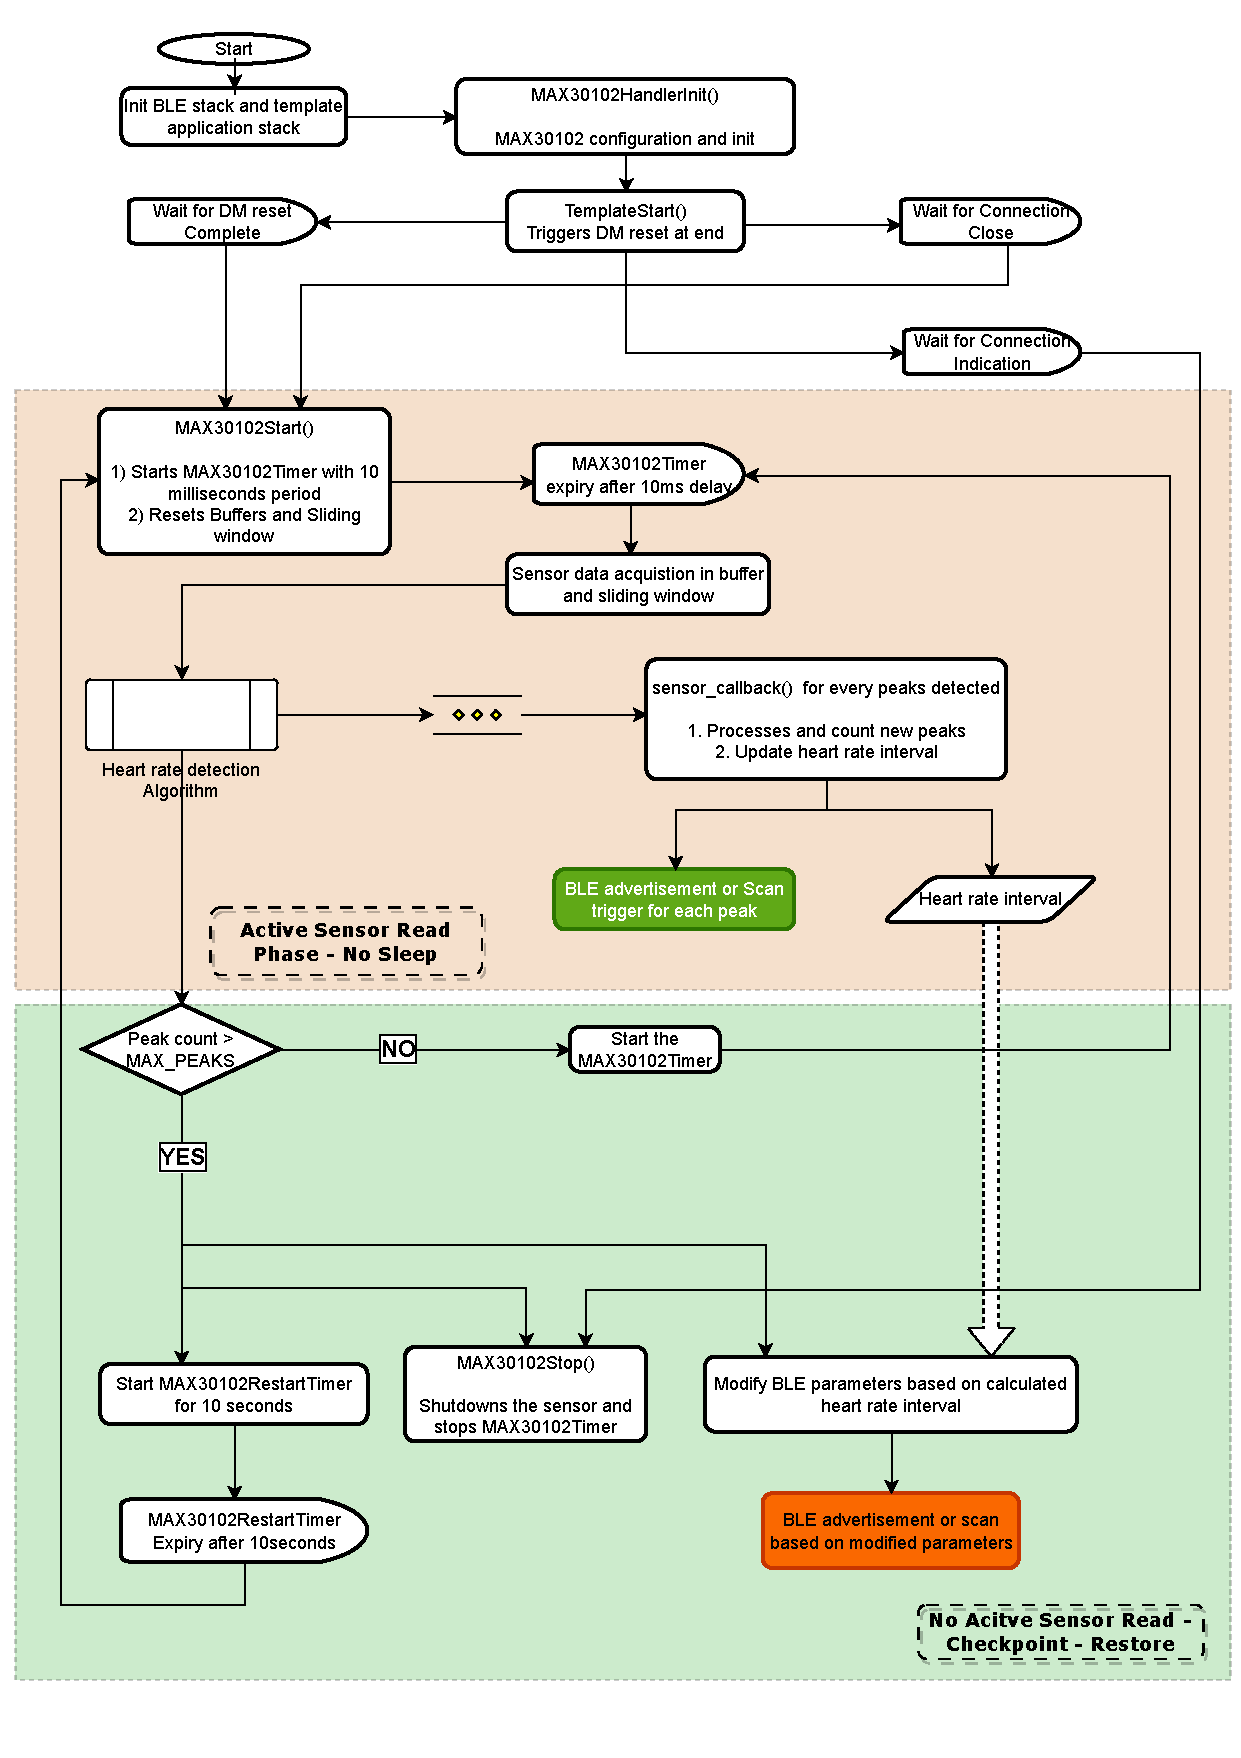
\includegraphics[width=\linewidth]{chapters/Implementation/Flowchart_CardioSync.pdf}
    \caption{Operation flowchart of the CardioSync framework implementation}
    \label{fig:flowchart}
\end{figure}
\chapter{Results and Evaluation}
\label{chap:results}

This chapter presents the results of experimentation, and analysis of data obtained from the CardioSync Framework. Also it compares the key result outcomes of CardioSync framework, such as \textit{BLE connection setup time, power and energy consumption} in comparison to a naive and reference Freebie system that does not employ any synchronisation mechanism. 
\vspace{1\baselineskip}

\noindent The evaluation of the CardioSync framework is structured into three distinct contexts, inline with the research objectives
\begin{enumerate}
    \item Heart Rate Sensor Accuracy and Peak detection Algorithm performance.

    \item Verification of Integrated CardioSync framework in Continuous and Intermittent power.

    \item Comparative analysis of CardioSync Framework vs. Naive Reference FreeBie model.
\end{enumerate}

\section{Evaluation of Heart Rate Sensor and Peak detection Algorithm}
\label{sec:sensor_performance}
The evaluation in this section is split into two parts - \textit{Sensor accuracy profiling} based on phase difference for a particular peak detected between two sensors and \textit{BLE connection performance} at different sensor sampling rate.

\subsection{Sensor Accuracy Profiling}
Sensor accuracy to detect heart beat is mainly based on the peak detection algorithm, and also on the configurations of the sensor. However, the sensor was intentionally designed to function within a fixed configuration, optimising power consumption (Refer to Section:\ref{sec:sensor_config} in Appendix \ref{app:appendix_a}). So to quantitatively assess accuracy of the algorithm, the phase difference for heart pulse detection between two sensors was selected as the focus. This parameter was examined across various sampling rates of the peak detection algorithm.

\subsubsection{Experimental Setup}
To measure the phase difference between the heart pulse detected by two different MAX30102 sensors and a nRF52840DK development board \cite{nRF52840} was used. The measurement software was developed based on nRF5 SDK \cite{2023nRF5} to interface with two sensor boards using two-wire interface (TWI).  The software would use the heart beat detection algorithm of the CardioSync system to independently identify heart pulse peaks for each sensor and log the corresponding detection time. Subsequently, the phase difference should be computed between the aforementioned peaks. After two sensors have recorded around 250 peak detection, an experiment is finished, and it is repeated four times, each time with different sensor sampling rates: \textit{25Hz, 50Hz, 100Hz, and 1000Hz}.

\subsubsection{Results Discussion}
\begin{figure}[t]
    \begin{subfigure}{0.5\linewidth}
        \centering
        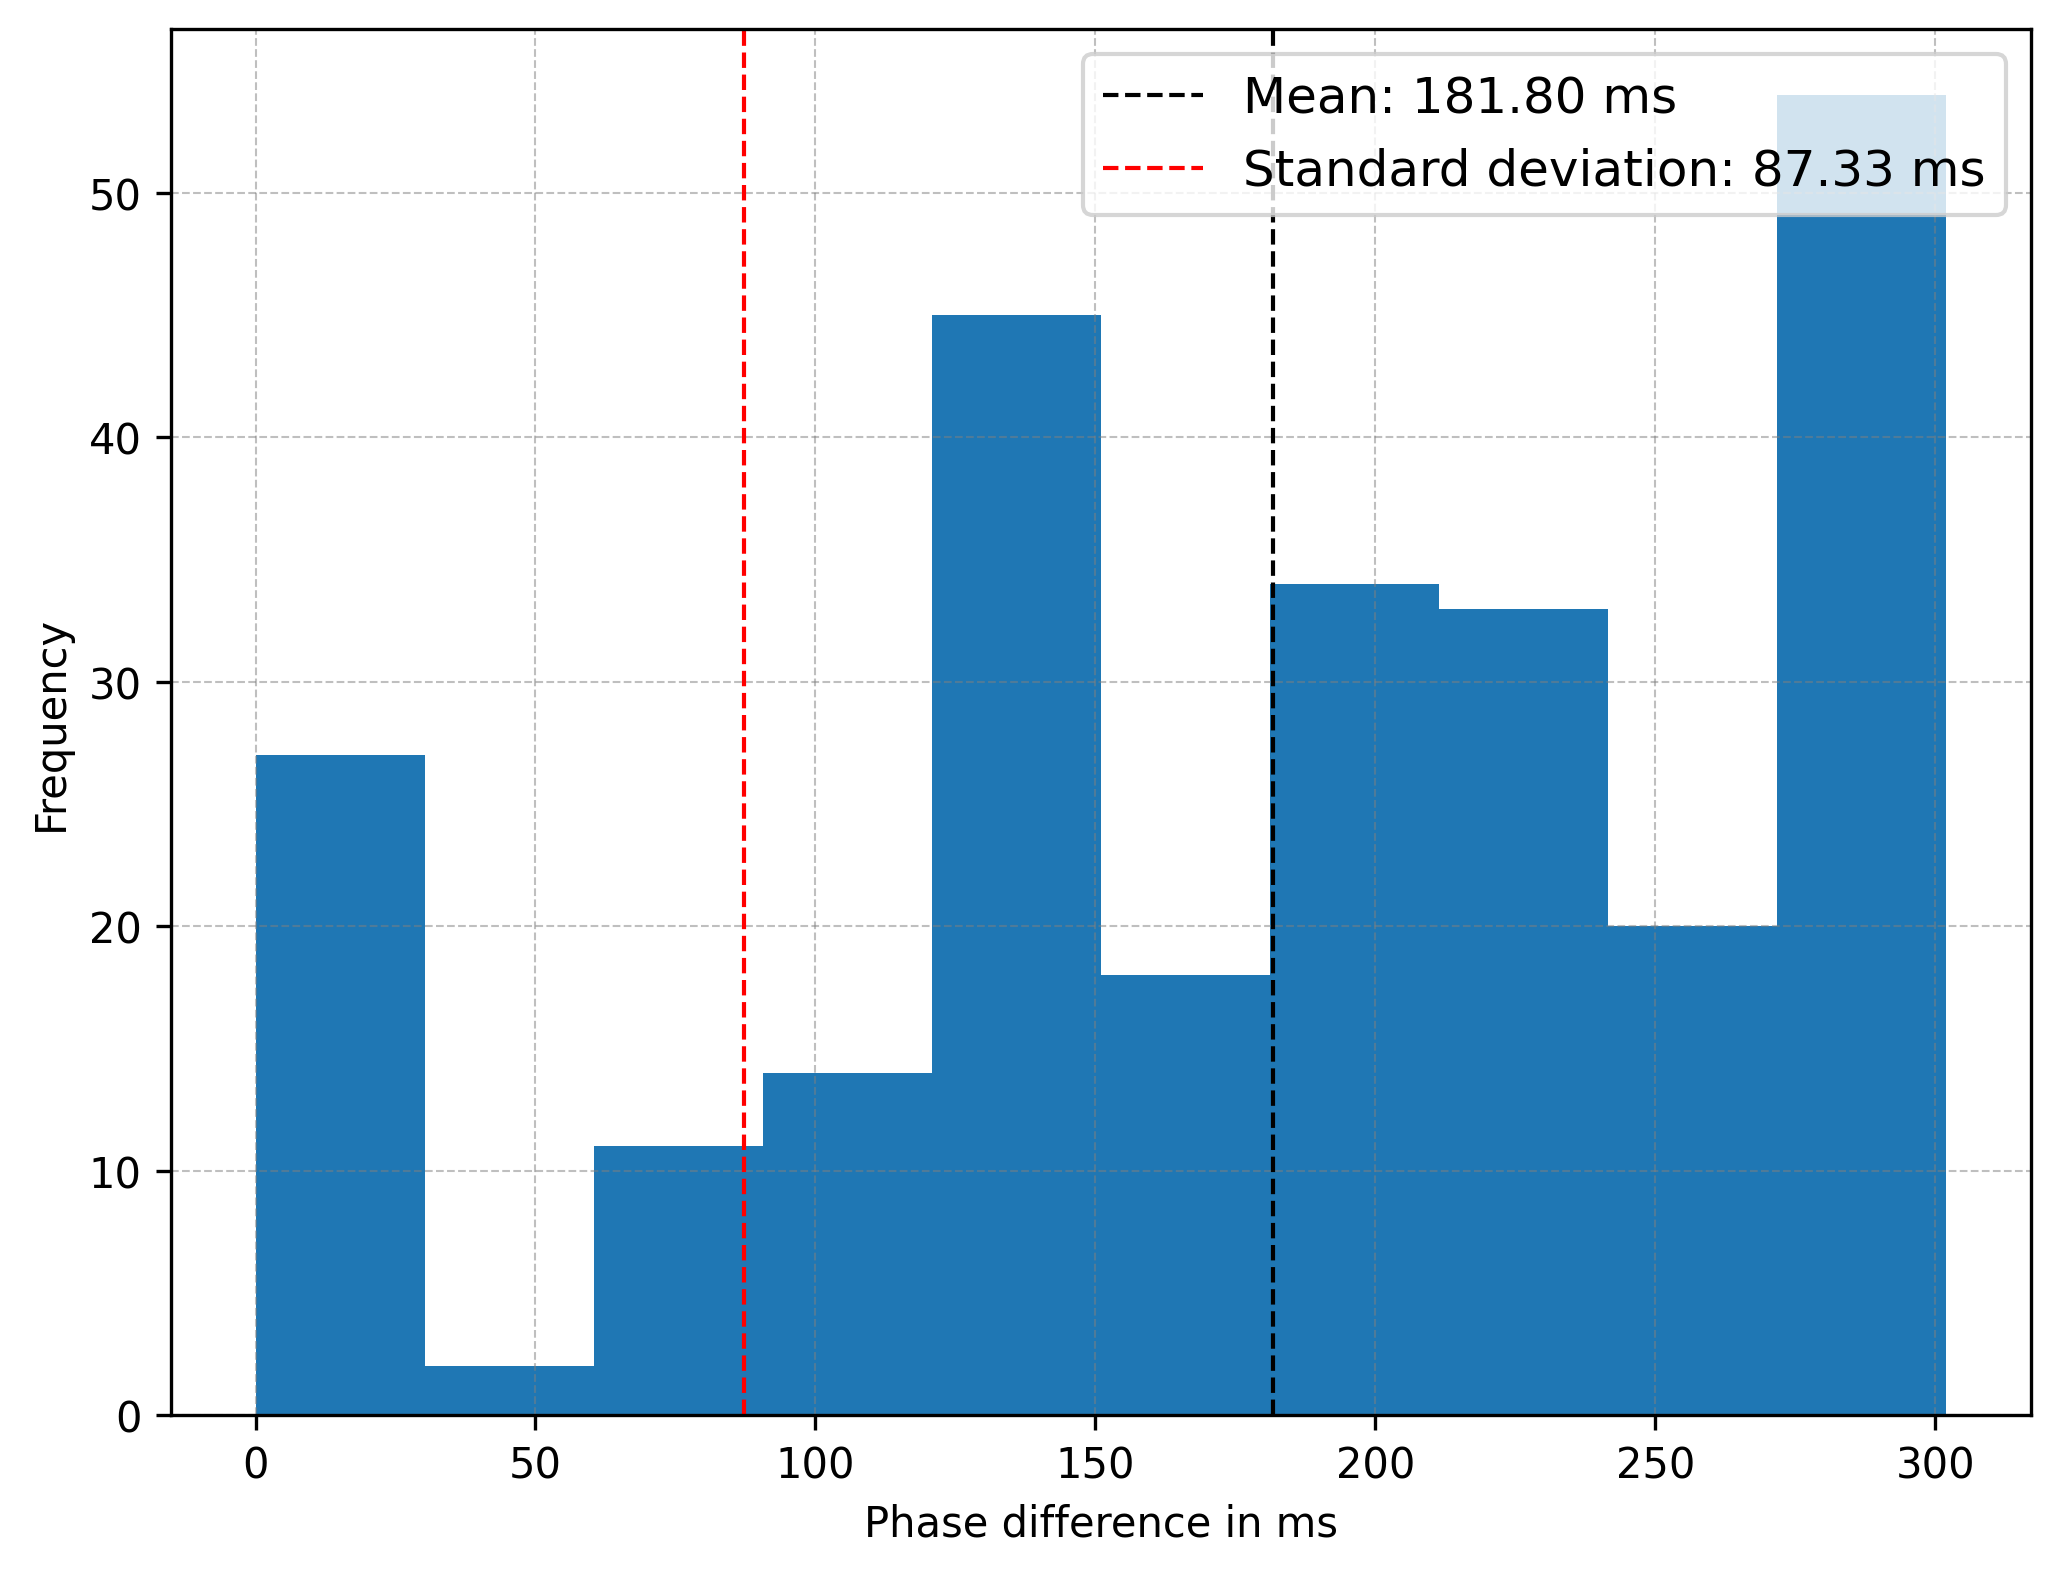
\includegraphics[width=\linewidth]{chapters/Results/histogram_25.png}
        \caption{25Hz}
        \label{fig:histogram_25}
        \vspace{1\baselineskip}
    \end{subfigure}
    \begin{subfigure}{0.5\linewidth}
        \centering
        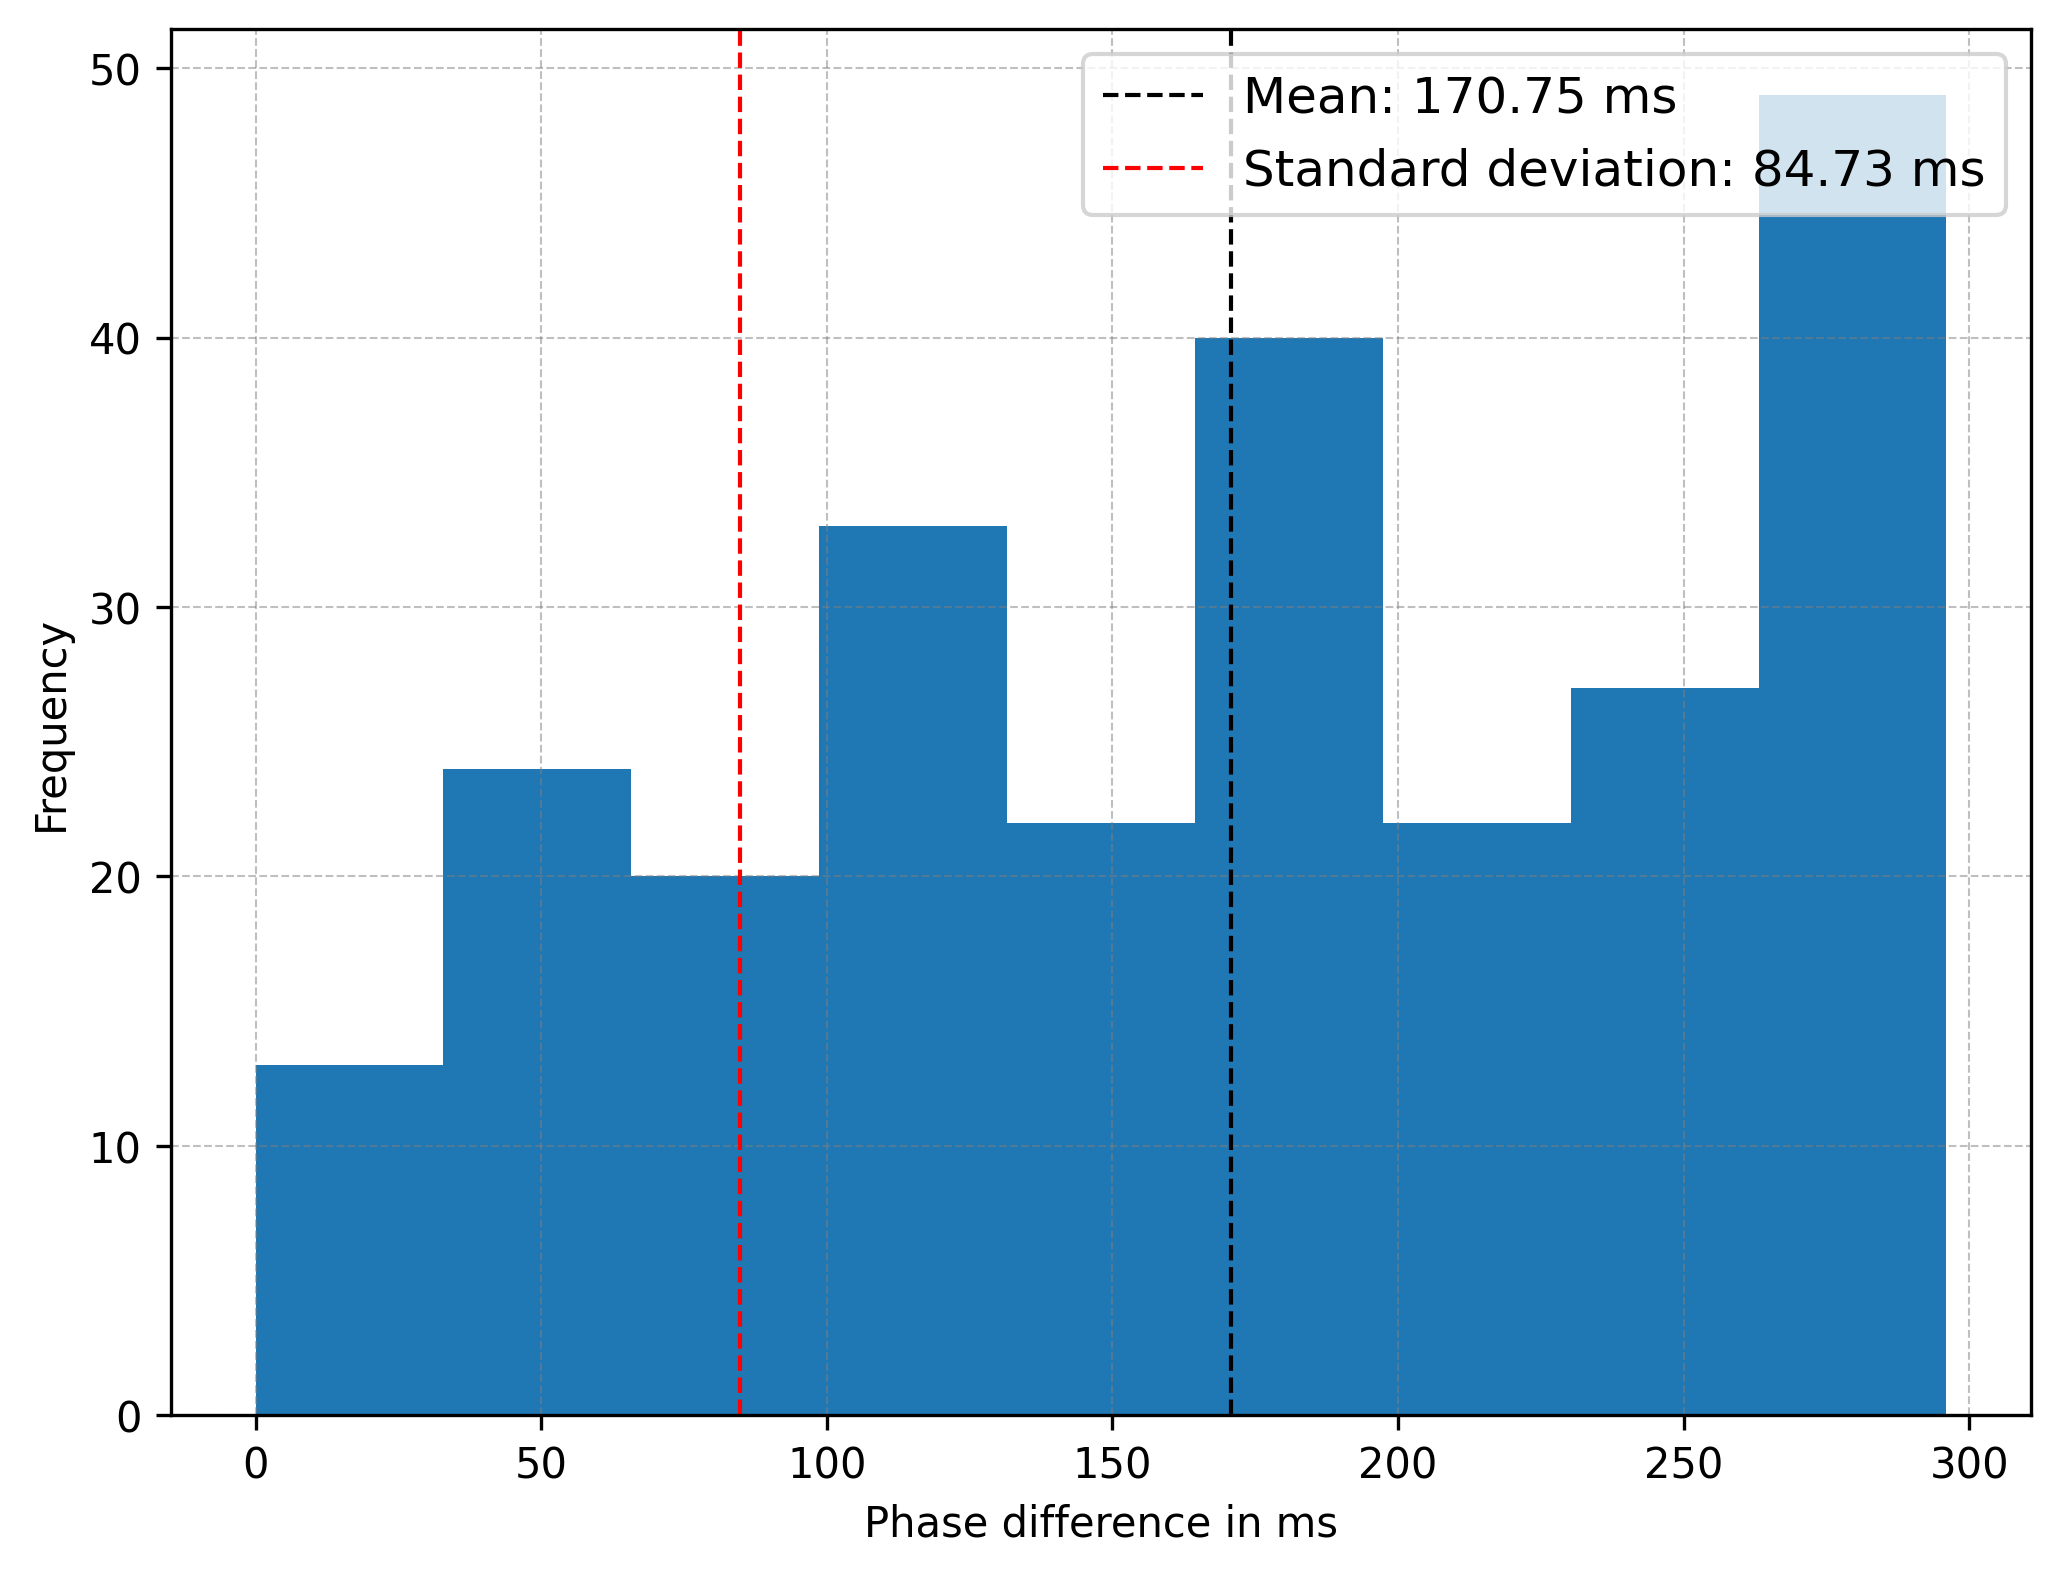
\includegraphics[width=\linewidth]{chapters/Results/histogram_50.png}
        \caption{50Hz}
        \label{fig:histogram_50}
        \vspace{1\baselineskip}
    \end{subfigure}
    \begin{subfigure}{0.5\linewidth}
        \centering
        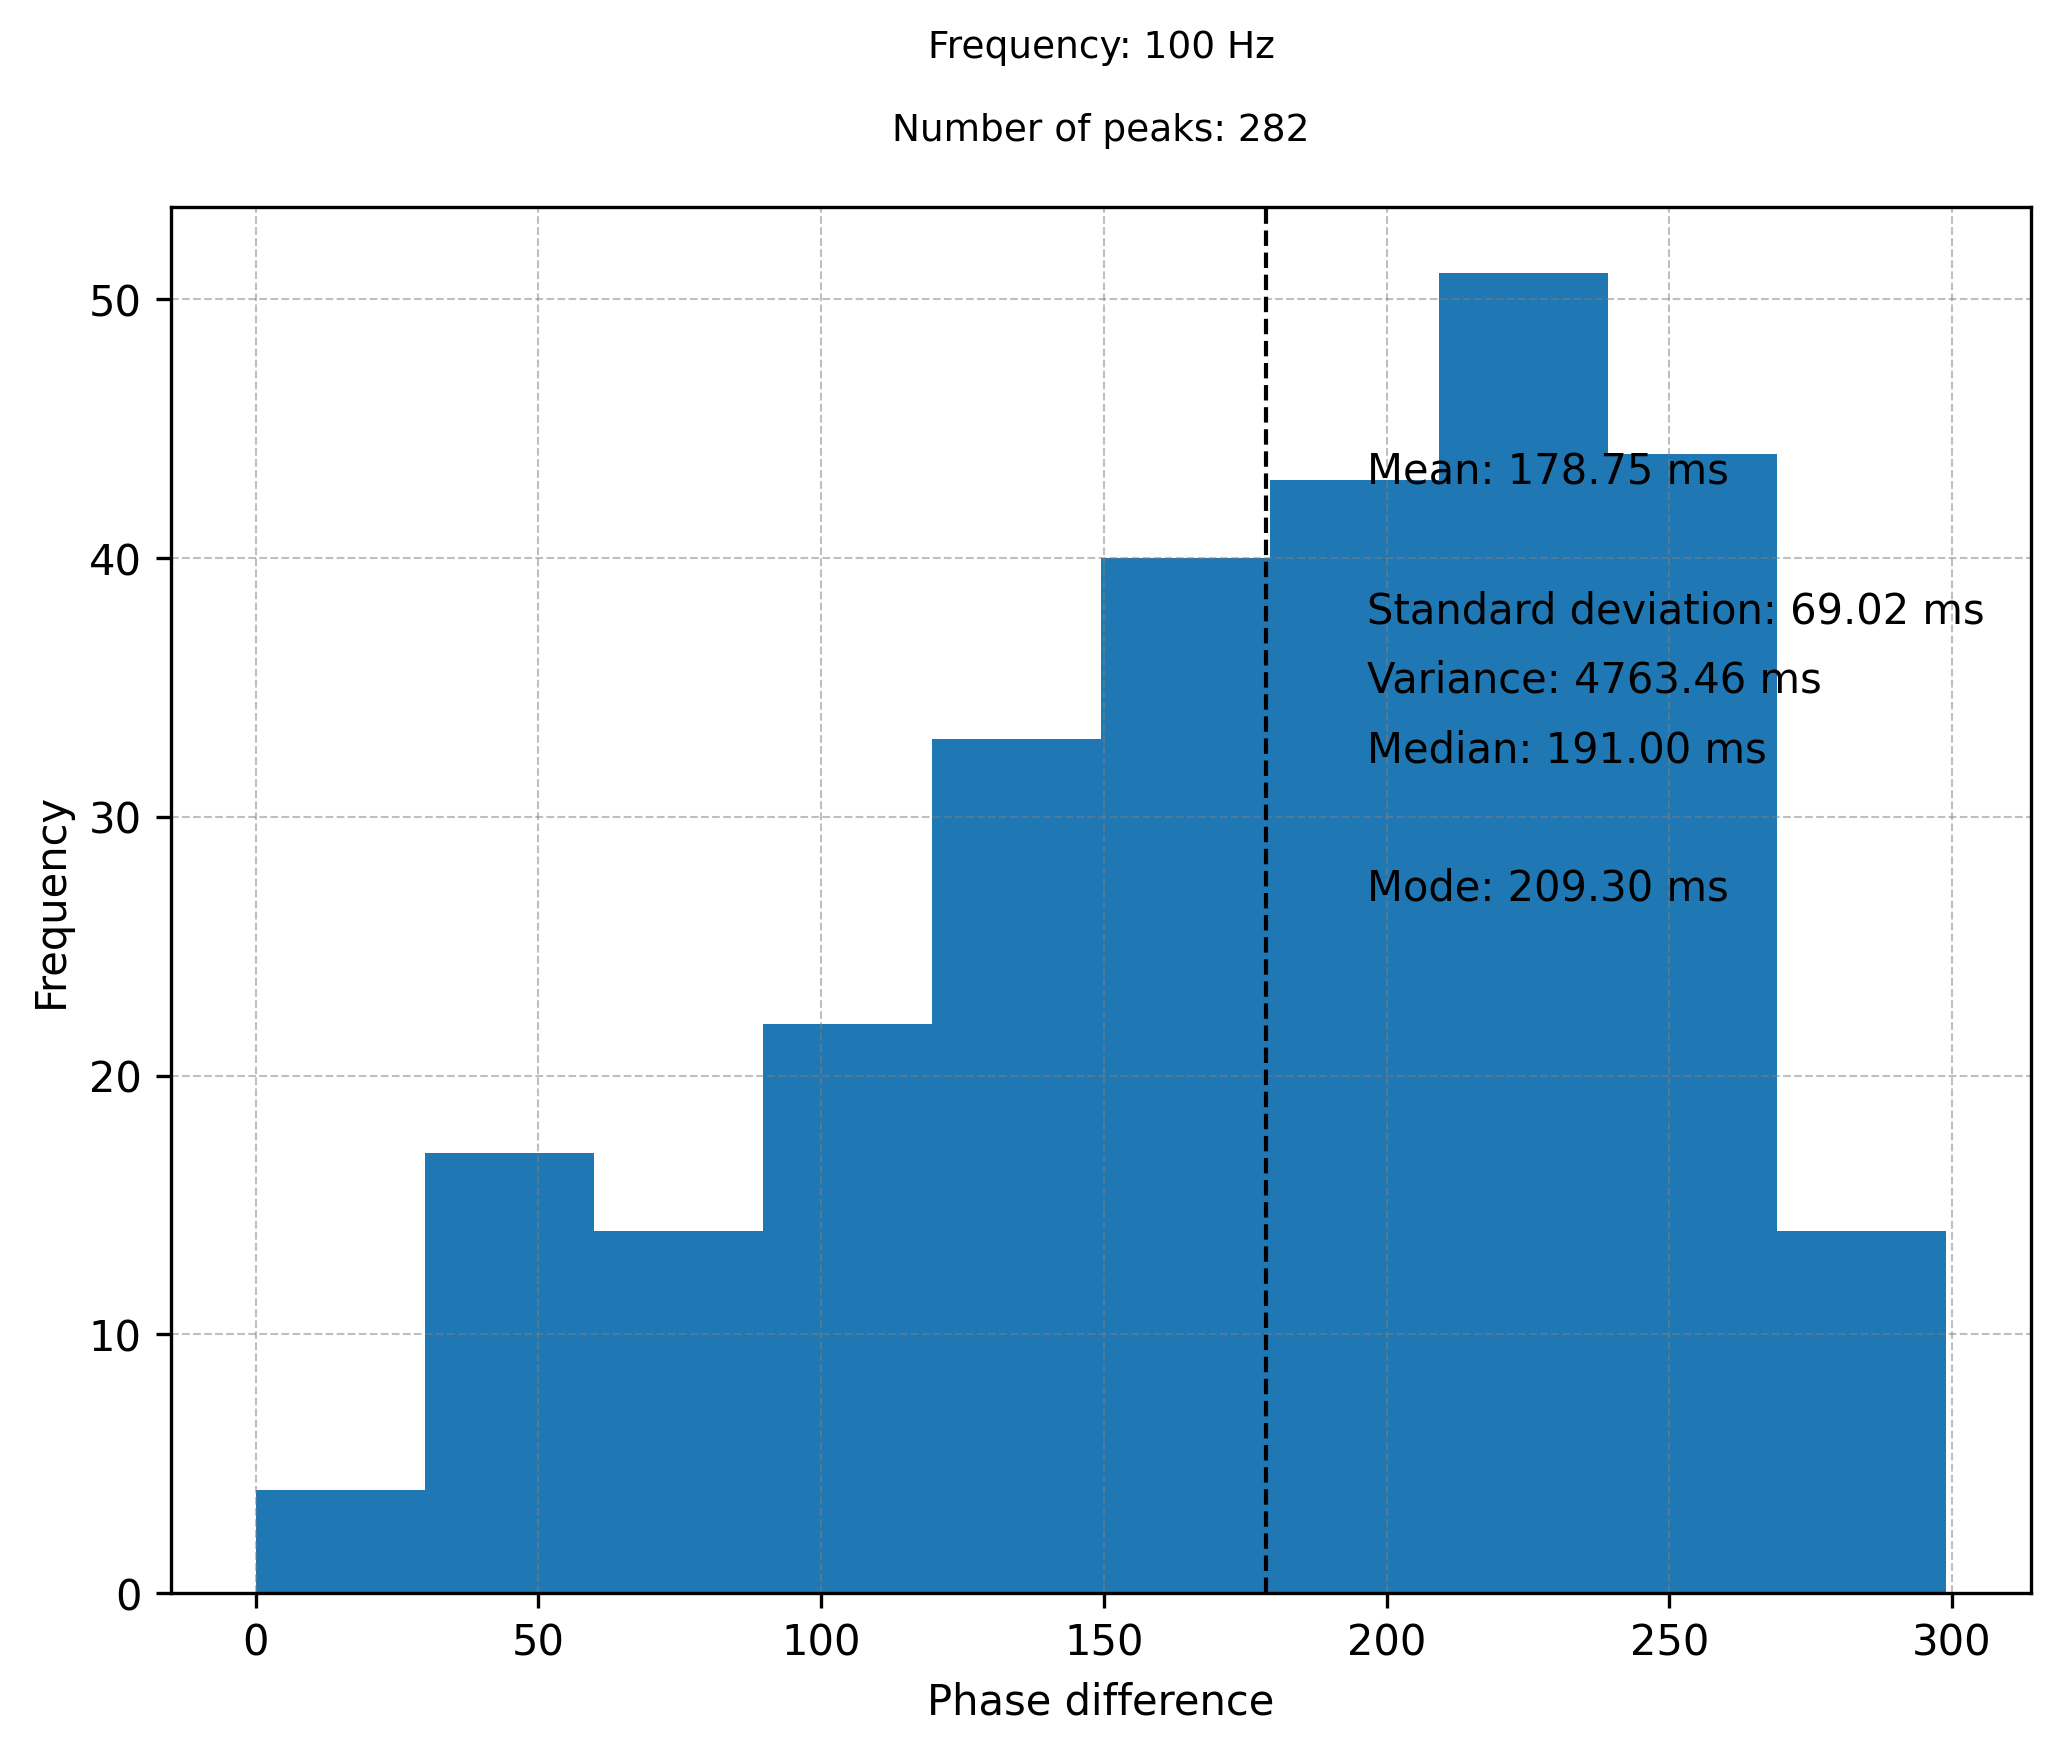
\includegraphics[width=\linewidth]{chapters/Results/histogram_100.png}
        \caption{100Hz}
        \label{fig:histogram_100}
    \end{subfigure}
    \begin{subfigure}{0.5\linewidth}
        \centering
        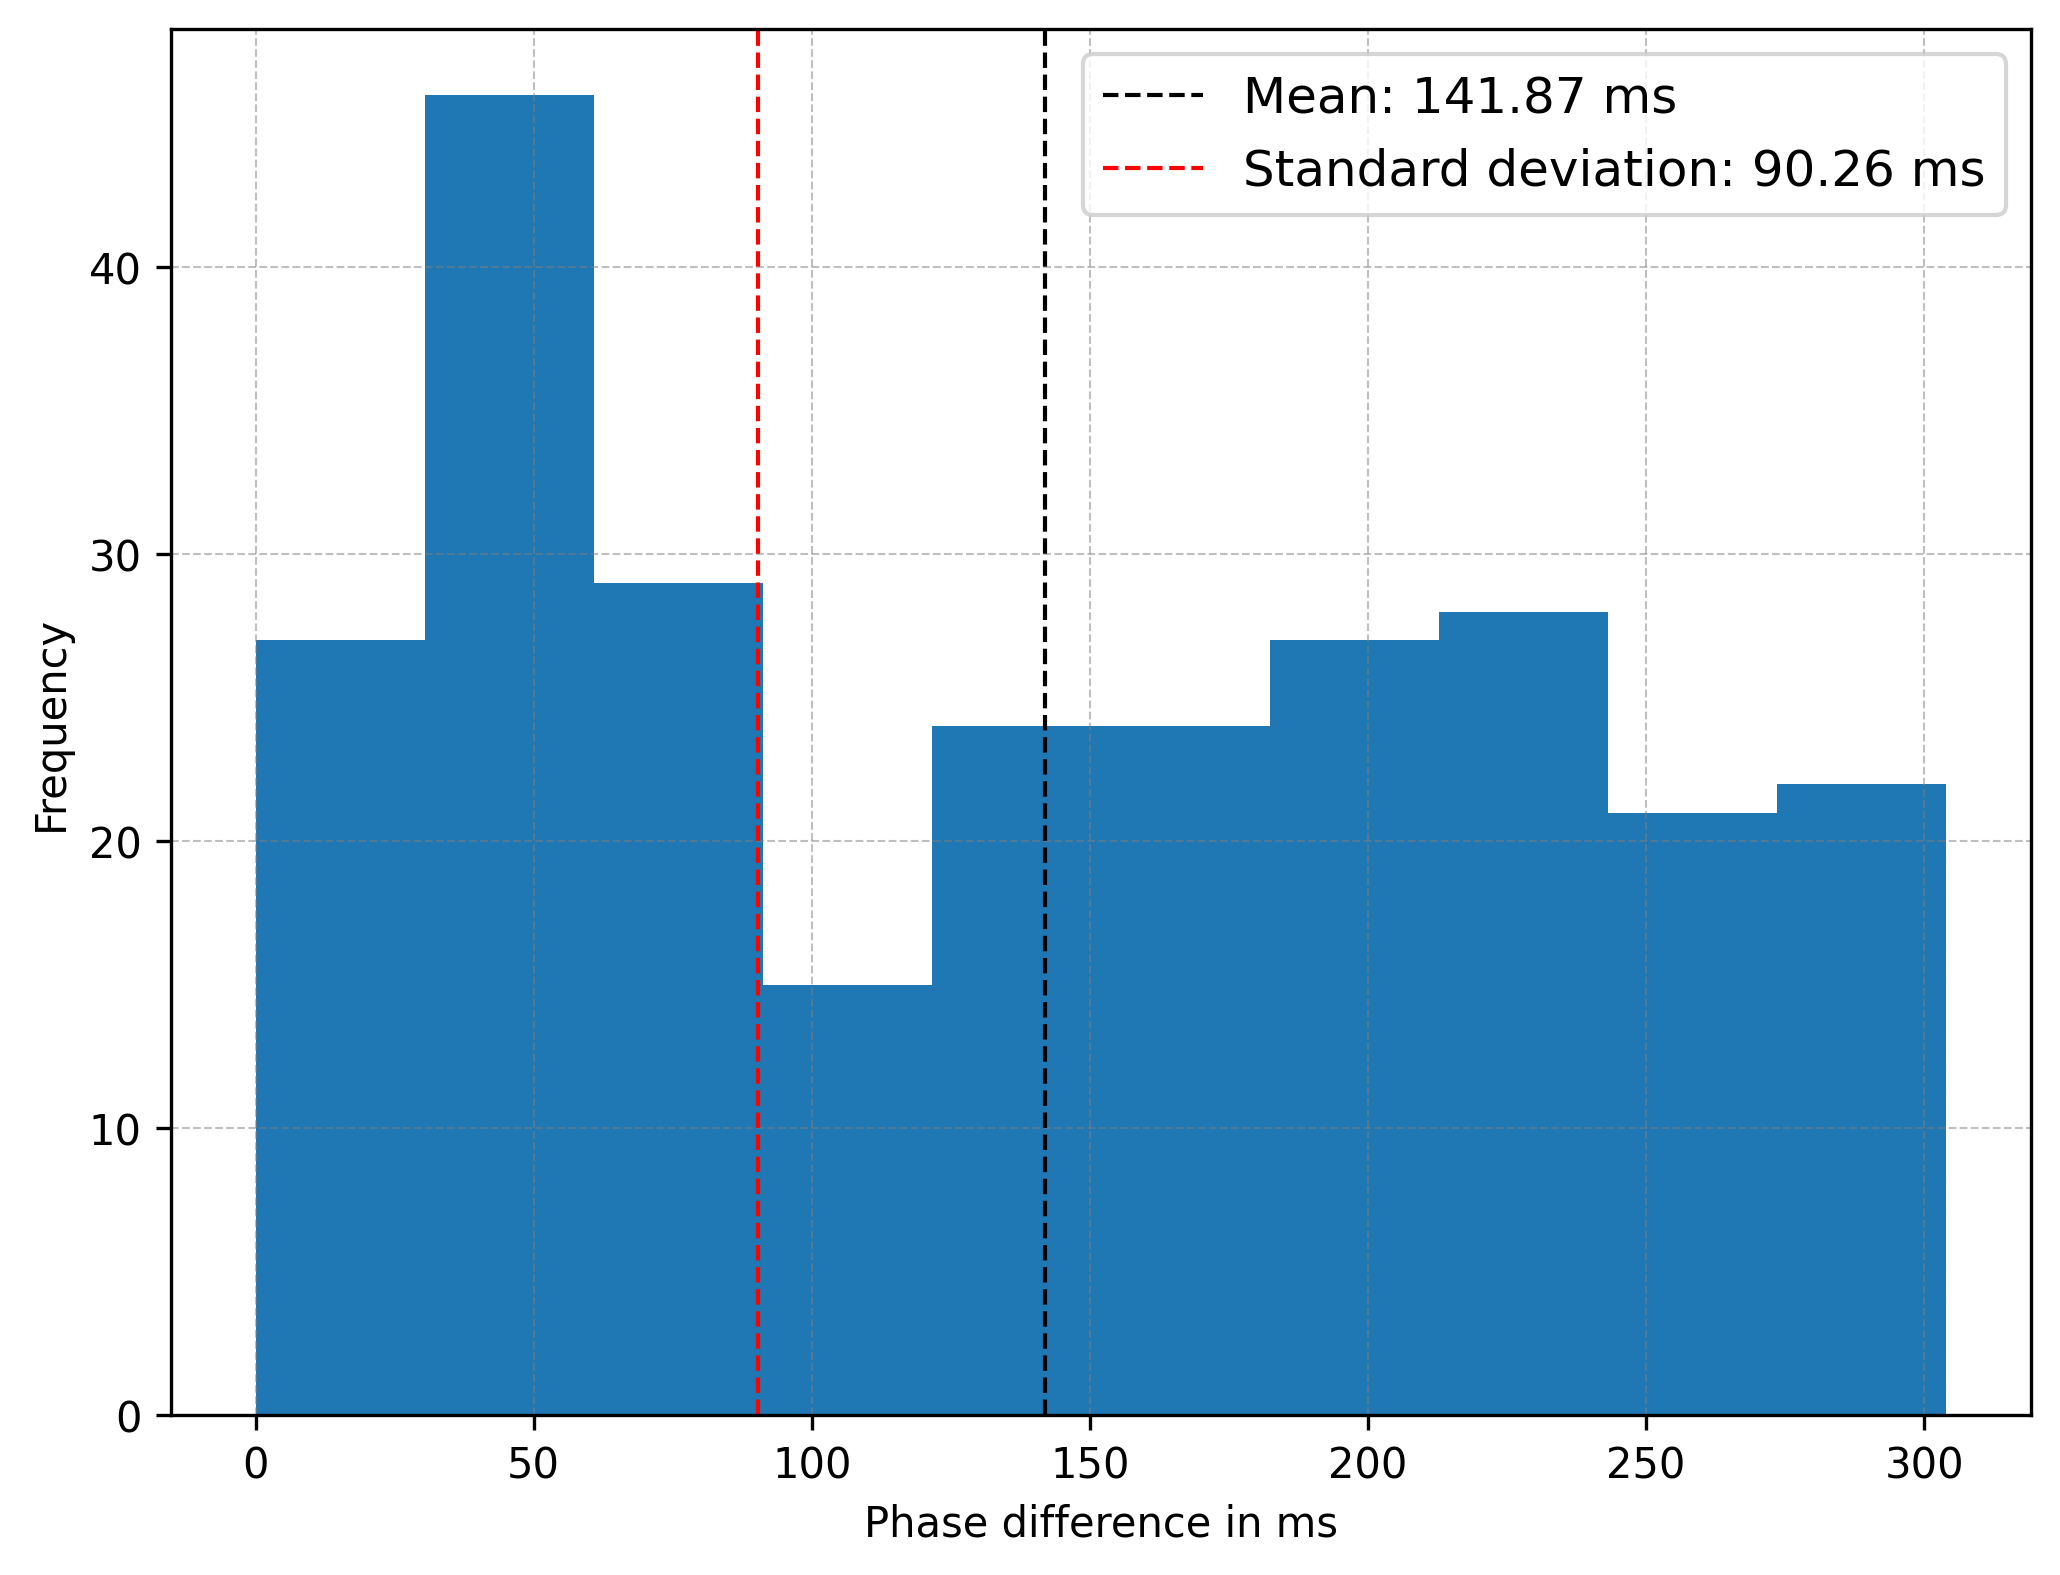
\includegraphics[width=\linewidth]{chapters/Results/histogram_1000.png}
        \caption{1000Hz}
        \label{fig:histogram_1000}
    \end{subfigure}
    \caption{Histograms of phase differences between heart pulses detected by two sensors at different sensor read frequencies. At 25 Hz and 50 Hz, larger phase differences occur at more frequency than 100 Hz. At 100 Hz, phase differences are evenly distributed around mean. At 100Hz, phases differences are more irregular.}
    \label{fig:histograms_sensor_accuracy}
\end{figure}

\begin{table}[t]
\centering
\begin{tabular}{|c|ccc|}
\hline
\multirow{2}{*}{\textbf{\begin{tabular}[c]{@{}c@{}}Sensor \\ Sampling rate\end{tabular}}} &
  \multicolumn{3}{c|}{\textbf{\begin{tabular}[c]{@{}c@{}}Phase difference\\ in milliseconds\end{tabular}}} \\ \cline{2-4} 
                 & \multicolumn{1}{c|}{\textbf{Mean}} & \multicolumn{1}{c|}{\textbf{Min}} & \textbf{Max} \\ \hline
25 Hz   & \multicolumn{1}{c|}{181.80}        & \multicolumn{1}{c|}{0}            & 301          \\ \hline
50 Hz   & \multicolumn{1}{c|}{170.75}        & \multicolumn{1}{c|}{0}            & 296          \\ \hline
100 Hz  & \multicolumn{1}{c|}{178.75}        & \multicolumn{1}{c|}{0}            & 299          \\ \hline
1000 Hz & \multicolumn{1}{c|}{141.87}        & \multicolumn{1}{c|}{0}            & 304          \\ \hline
\end{tabular}
\caption{Phase difference statistics at different sensor sampling rates.}
\label{tab:phase_difference_comp}
\end{table}

The histograms shown in Figure \ref{fig:histograms_sensor_accuracy} illustrate the distribution of phase differences recorded for various sensor sampling rates. The mean, minimum, and maximum phase differences are summarised in \autoref{tab:phase_difference_comp}. Analysing these distributions and their statistical characteristics reveals that phase difference in detection time between two sensors is inevitable. However, this data holds valuable insights for determining the optimal sensor read frequency for the CardioSync system.
\vspace{1\baselineskip}

\noindent At different sampling rates (25Hz, 50Hz, 100Hz, and 1000Hz), the distribution of phase differences between heart rate peaks reveals distinct characteristics. At 25Hz and 50Hz, a right-skewed distribution indicates a higher likelihood of larger phase differences, with about 33\% and 35\% of detected peaks respectively being more than 305ms out of phase. In contrast, a slightly right-skewed normal distribution at 100Hz suggests that phase differences mostly occur around the mean value, with around 24\% exceeding the 305ms threshold. A 1000Hz sampling rate presents an irregular phase difference distribution, highlighting unpredictable occurrences.
\vspace{1\baselineskip}

\noindent From all these observations, it can be concluded that \textbf{\textbf{Sampling rate 100Hz}} is more predictable in terms of phase difference and is more accurate in heart pulse peak detection between two sensors. Also, even the sensor settings are at 50 samples per second, thereby not losing any samples from the sensor.



\subsection{BLE connection performance}

\noindent The aim of this assessment is to analyse the performance of the novel CardioSync peak detection algorithm with the synchronised Bluetooth Low Energy (BLE) connection at different sensor sampling rates. This evaluation is conducted in preparation for the integration of the algorithm into the FreeBie architecture. The analysis was based on the number of peaks needed for successful connection establishment.

\subsubsection{Experimental Setup}
To record the number of heart pulse peaks needed for successful BLE connection, two nRF52840DK development board \cite{nRF52840} were used and each board was interfaced with one MAX30102 sensor \cite{2018MAX30102} to its I2C GPIO pins. Measurement software was developed based on the PacketCraft BLE stack \cite{2020Packetcraft}. The devised measurement code calculates the average time interval between peaks detected by the algorithm in run time. Also once the connection is established, it records the number of peaks detected before connection.
\vspace{1\baselineskip}

\noindent With these setup, 15 experiments were performed at different sensor sampling frequencies. Each experiment is considered complete once the connection is established between two nRF52840DK boards using the MAX30102 detected heart pulses.

\subsubsection{Results Discussion}

\begin{table}[t]
\centering
\begin{tabular}{|c|cc|cc|}
\hline
\multirow{2}{*}{\textbf{\begin{tabular}[c]{@{}c@{}}Sensor \\ Sampling rate\end{tabular}}} &
  \multicolumn{2}{c|}{\textbf{\begin{tabular}[c]{@{}c@{}}Average number \\ of peaks detected \\ to connect\end{tabular}}} &
  \multicolumn{2}{c|}{\textbf{\begin{tabular}[c]{@{}c@{}}Average\\ Connection setup time\\ in seconds\end{tabular}}} \\ \cline{2-5} 
                 & \multicolumn{1}{c|}{\textbf{Peripheral}} & \textbf{Central} & \multicolumn{1}{c|}{\textbf{Peripheral}} & \textbf{Central} \\ \hline
50 Hz   & \multicolumn{1}{c|}{1.6}                 & 1.6              & \multicolumn{1}{c|}{2.789}               & 2.847            \\ \hline
100 Hz  & \multicolumn{1}{c|}{1.667}               & 1.733            & \multicolumn{1}{c|}{2.074}               & 2.018            \\ \hline
1000 Hz & \multicolumn{1}{c|}{1.8667}              & 1.733            & \multicolumn{1}{c|}{1.407}               & 1.129            \\ \hline
\end{tabular}
\caption{Comparison of BLE connection at different sensor sampling rates. Number of peaks detected before connection setup occurs is lesser at 100 Hz than 1000 Hz, even though the average connection setup time is lower at 1000 Hz.}
\label{tab:ble_conn_comp}
\end{table}


\begin{table}[t]
\centering
\begin{tabular}{|cc|}
\hline
\multicolumn{2}{|c|}{\textbf{\begin{tabular}[c]{@{}c@{}}BLE Advertisement Parameters\\ (Peripheral)\end{tabular}}} \\ \hline
\multicolumn{1}{|c|}{\textit{Advertising Interval}} & 50 milliseconds  \\ \hline
\multicolumn{1}{|c|}{\textit{Advertising Duration}} & 200 milliseconds \\ \hline
\multicolumn{2}{|c|}{\textbf{\begin{tabular}[c]{@{}c@{}}BLE Scan Parameters\\ (Central)\end{tabular}}}             \\ \hline
\multicolumn{1}{|c|}{\textit{Scan Interval}}        & 15 milliseconds  \\ \hline
\multicolumn{1}{|c|}{\textit{Scan Window}}          & 20 milliseconds  \\ \hline
\multicolumn{1}{|c|}{\textit{Scan Duration}}        & 200 milliseconds \\ \hline
\end{tabular}
\caption{Chosen BLE parameters for the CardioSync system based on chosen sampling rate 100 Hz.}
\label{tab:ble_params}
\end{table}

The results in \autoref{tab:ble_conn_comp} demonstrate that a sampling frequency of 1000Hz results in a shorter average time interval between peaks, enhancing connection establishment time due to quicker peak detection. However, this frequency exhibited an inconsistent number of peaks between experiments for connection establishment, leading to a higher average number of required peaks. Consequently, balancing these findings with the earlier assessment of sensor accuracy, \textbf{the 100Hz sampling rate was selected for integrating the CardioSync system}.
\vspace{1\baselineskip}

\noindent Furthermore, the selection of a sample frequency of 100Hz has led to the determination of BLE parameters for the CardioSync system, backed up by the outcomes of this evaluation. In order to address the \textbf{average phase difference of 178.75 milliseconds} observed between two sensors and reducing the number of peaks necessary to establish a connection, the BLE advertising and scanning configurations have been chosen as outlined in Table \ref{tab:ble_params}. 
\vspace{1\baselineskip}

\noindent Both the scan and advertising duration have been set at 200 milliseconds for each detected heart pulse. This allows for a sufficient window of time to synchronise and establish a connection, even in cases where there may be a significant disparity between the readings from two sensors.


\section{Validation of Integrated CardioSync System}
The purpose of the following section is to provide an illustration of the operational functionality of the integrated CardioSync framework to synchronise a BLE connection setup within sleep-wakeup principles of the FreeBie system architecture. The findings are presented for two types of input power: Continuous power and Intermittent power (which were emulated using a square wave and the parameters of the square wave are 75\% duty cycle and total period of 8 seconds).

\subsection{Experimental Setup}
\label{sec:experimental_setup}
\subsubsection{Hardware Setup}
The experimental configuration comprises of two FreeBie boards \cite{Researchers}, each equipped with a MAX30102 sensor. The voltage supplied to the sensor is derived from the \(\text{V}_\text{Batt}\) source on the FreeBie board. The FreeBie board receives its voltage supply from a voltage emulator kit called \textit{DIPS} \cite{DIPSGitHub} connected to the \(\text{V}_\text{Store}\) pin. The DIPS system comes with Emulator Host software, which facilitates the configuration and simulation of the desired voltage supply for the FreeBie system \cite{DIPSGitHub}.
\vspace{1\baselineskip}

\noindent The \textit{Saleae logic analyser} \cite{LogicAnalyser} is employed to gather results that demonstrate the functionality of the system. In our experimental setup, we employed four channels from logic analyser for each of the FreeBie boards to measure the voltage values of \textit{\(\text{V}_\text{DD\_MCU}\), \(\text{V}_\text{Store}\), Sensor Read state(GPIO pin), and Connection Open indication (GPIO pin)}.
\vspace{1\baselineskip}

\noindent The \textit{nRF Power Profiler Kit II (PPK)} \cite{2023Power} is employed for the purpose of measuring energy consumption throughout the runtime by hooking it to the \(\text{V}_\text{Store}\) pin of the board. Additionally, it serves as a continuous source of power for the FreeBie board. Similar to the Saleae Logic analyser, the PPK is capable of capturing and recording current measurements of a device in real-time.

\subsubsection{Software Setup}
Regarding the experimental software setup, modifications have been made to the system described in Chapter \ref{chap:implementation}. These modifications involve the activation of two GPIO pins to indicate the start and stop of the sensor read phase and the successful establishment of a BLE connection respectively. One of the FreeBie board is programmed with the CardioSync Peripheral code, while the other is flashed with the CardioSync Central code.

\subsection{Results Discussion}

\begin{figure}[ht]
    \begin{subfigure}{1\linewidth}
        \centering
        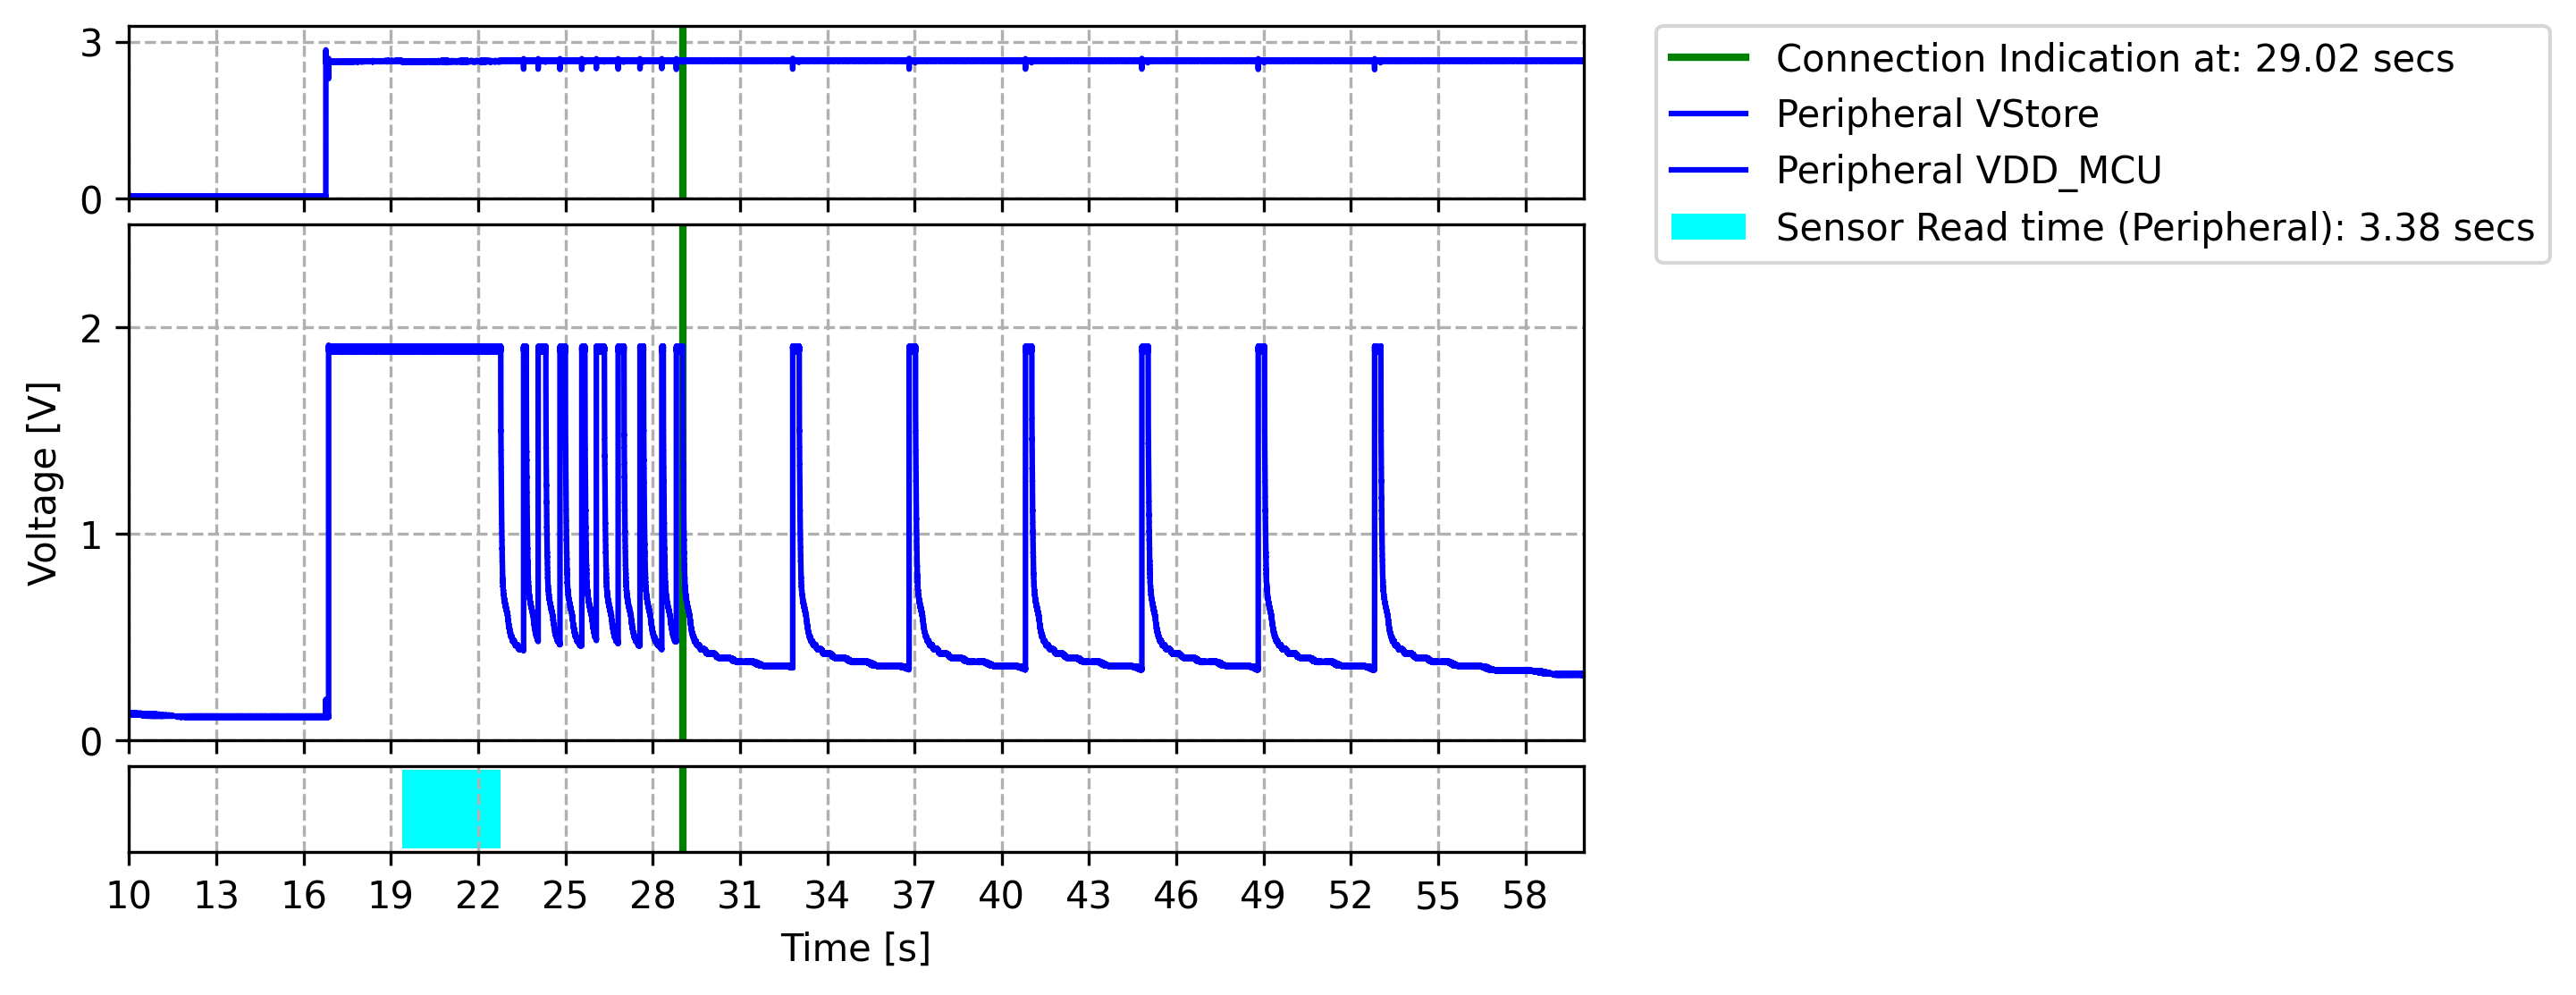
\includegraphics[width=1\linewidth]{chapters/Results/Connection_cardiosync_continous_peripheral.png}
        \caption{Voltage measurement for peripheral device.}
        \label{fig:continous_connection_cardiosync_peripheral}
        \vspace{1\baselineskip}
    \end{subfigure}
    \begin{subfigure}{1\linewidth}
        \centering
        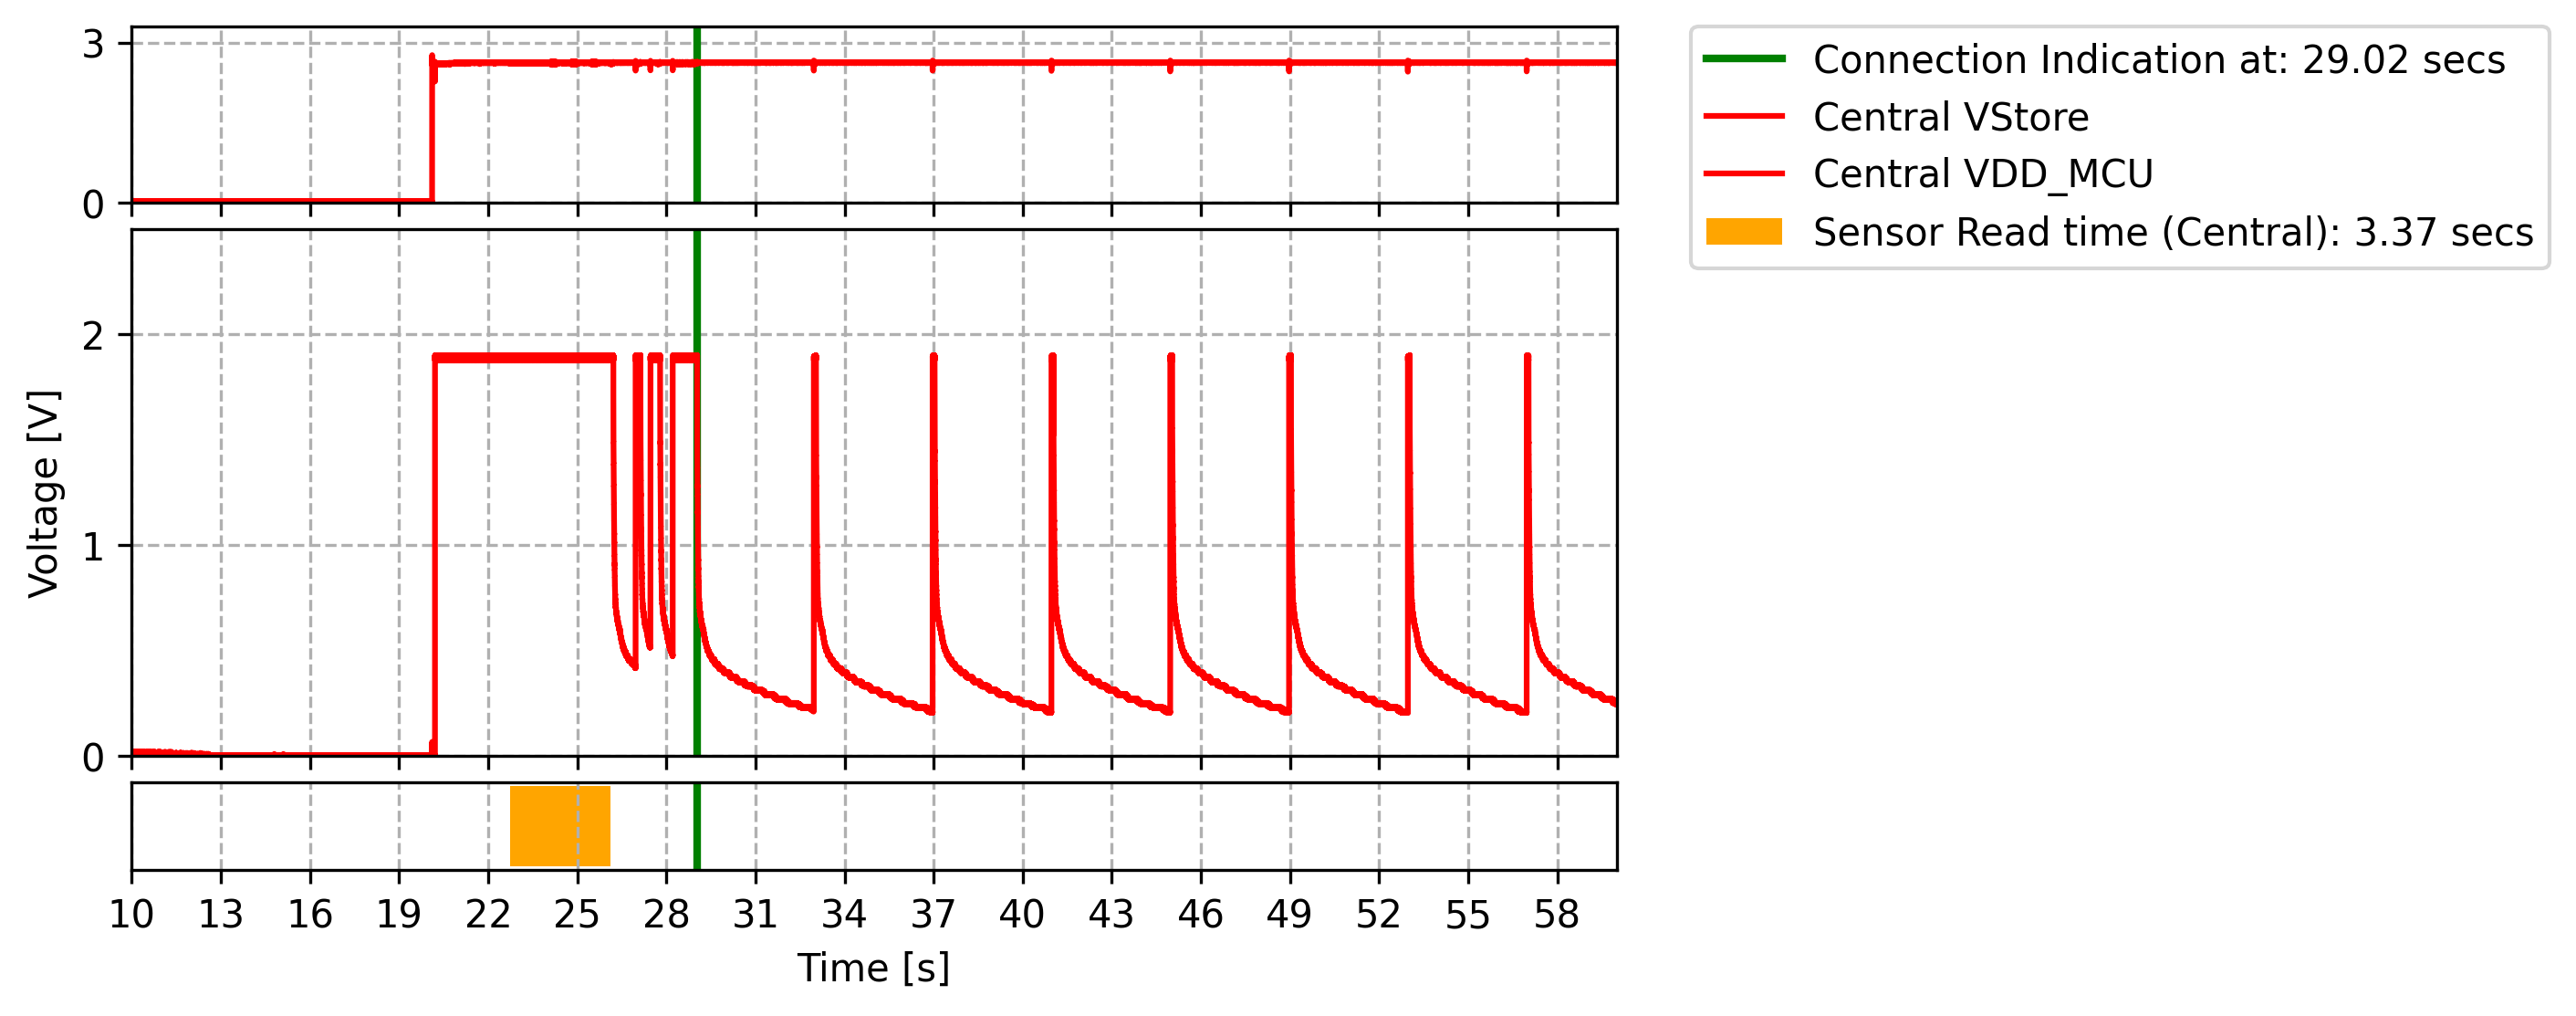
\includegraphics[width=1\linewidth]{chapters/Results/Connection_cardiosync_continous_central.png}
        \caption{Voltage measurement for central device.}
        \label{fig:continous_connection_cardiosync_central}
    \end{subfigure}
    \caption{Real-time voltage measurement for the CardioSync system \textit{with continuous power supply}. Each of the three plot in two devices shows different measurement. From the top to bottom in each device, 1) Plot of \(\text{V}_\text{Store}\) : Supply Voltage, 2) Plot of \(\text{V}_\text{DD\_MCU}\) : MCU voltage and 3) Plot of sensor read period indication. The green vertical line through all the plots indicates the successful BLE connection setup event.}
    \label{fig:continous_connection_cardiosync}
\end{figure}

\begin{figure}[ht]
    \begin{subfigure}{1\linewidth}
        \centering
        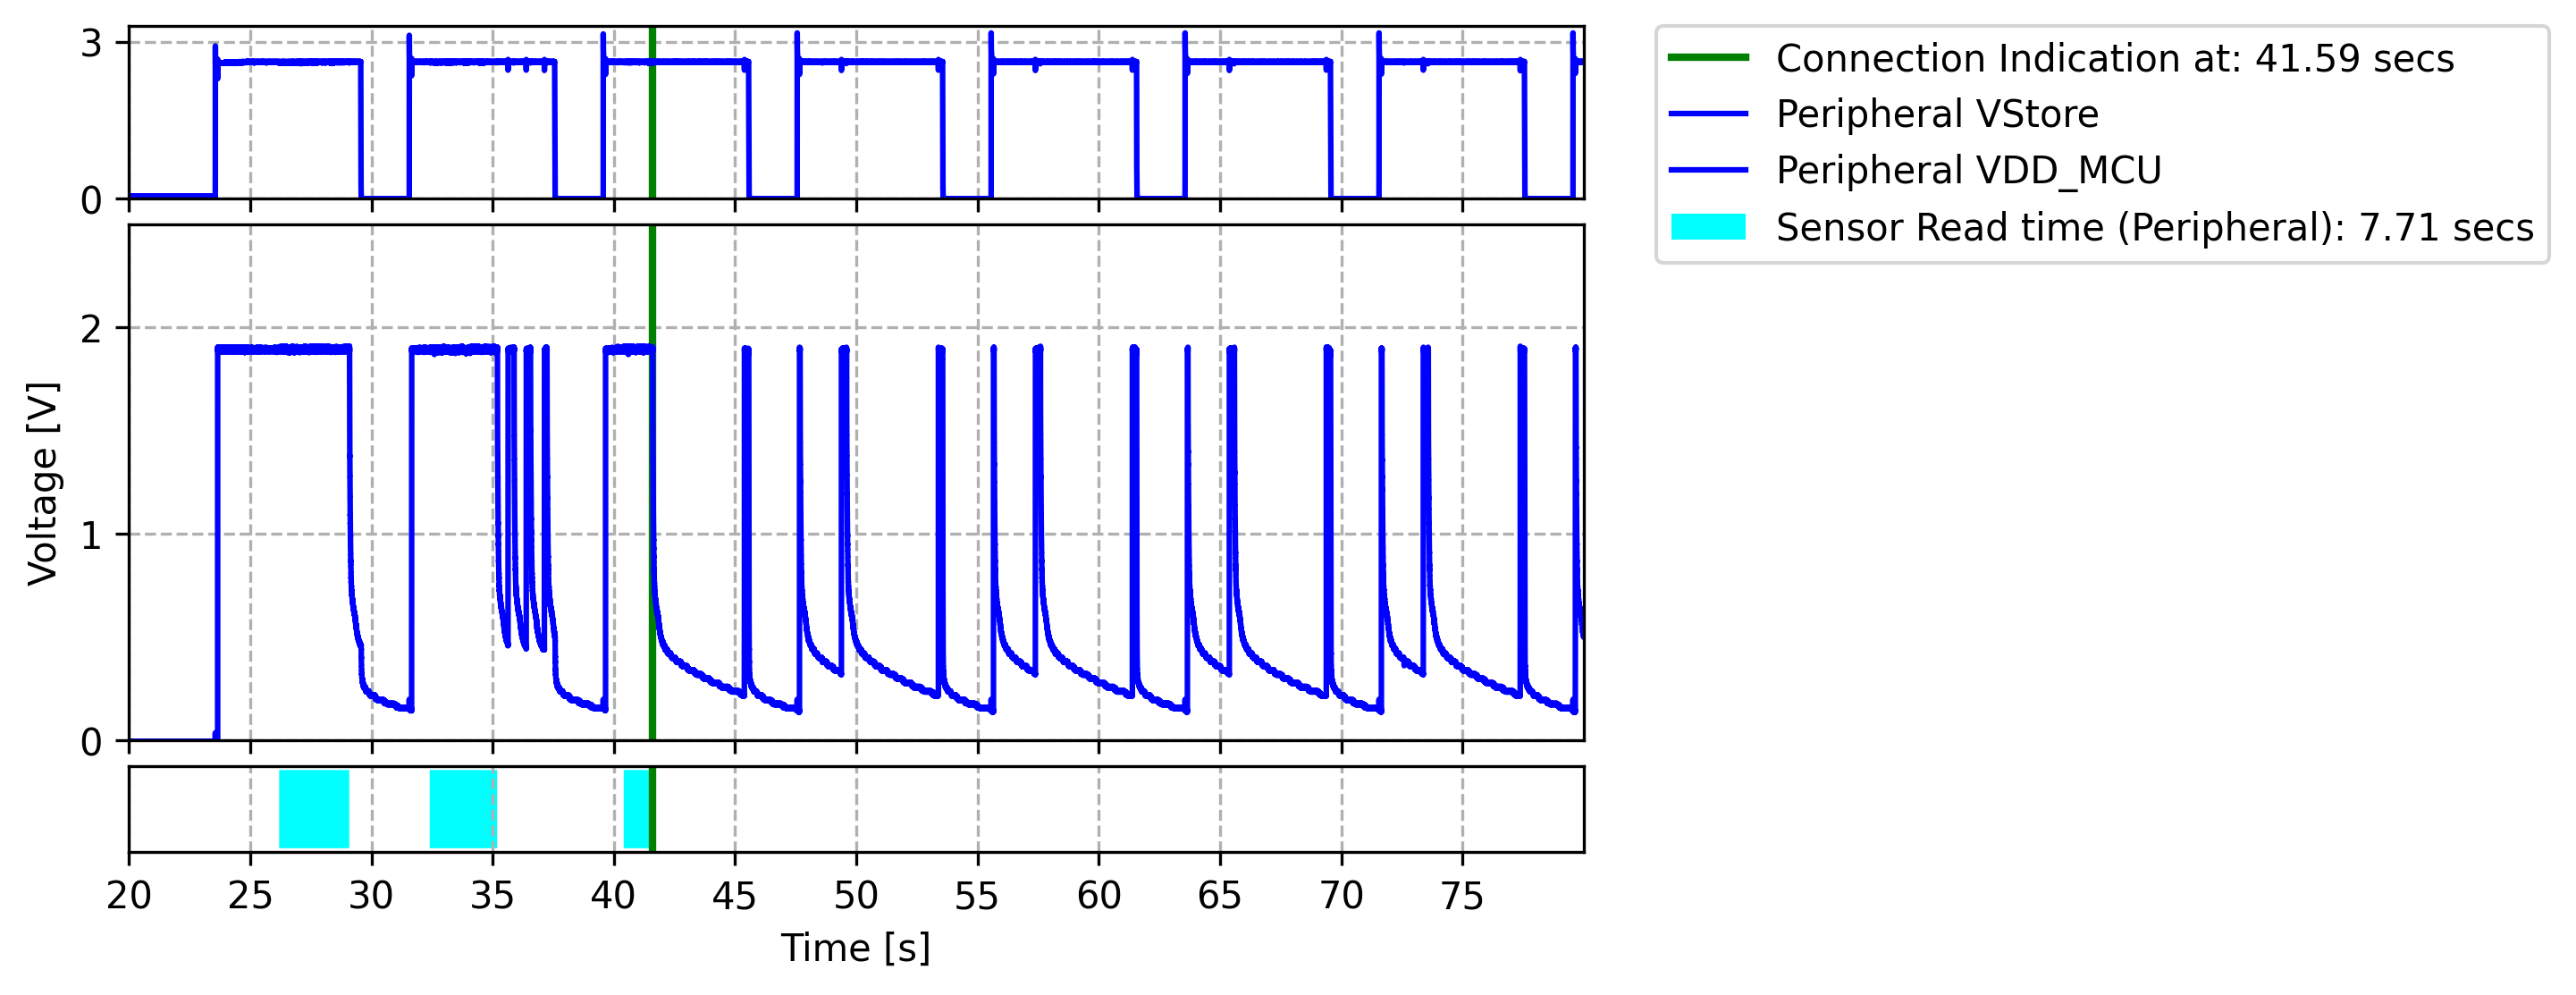
\includegraphics[width=1\linewidth]{chapters/Results/Connection_cardiosync_intermittent_peripheral.png}
        \caption{Voltage measurement for peripheral device.}
        \label{fig:intermittent_connection_cardiosync_peripheral}
        \vspace{1\baselineskip}
    \end{subfigure}
    \begin{subfigure}{1\linewidth}
        \centering
        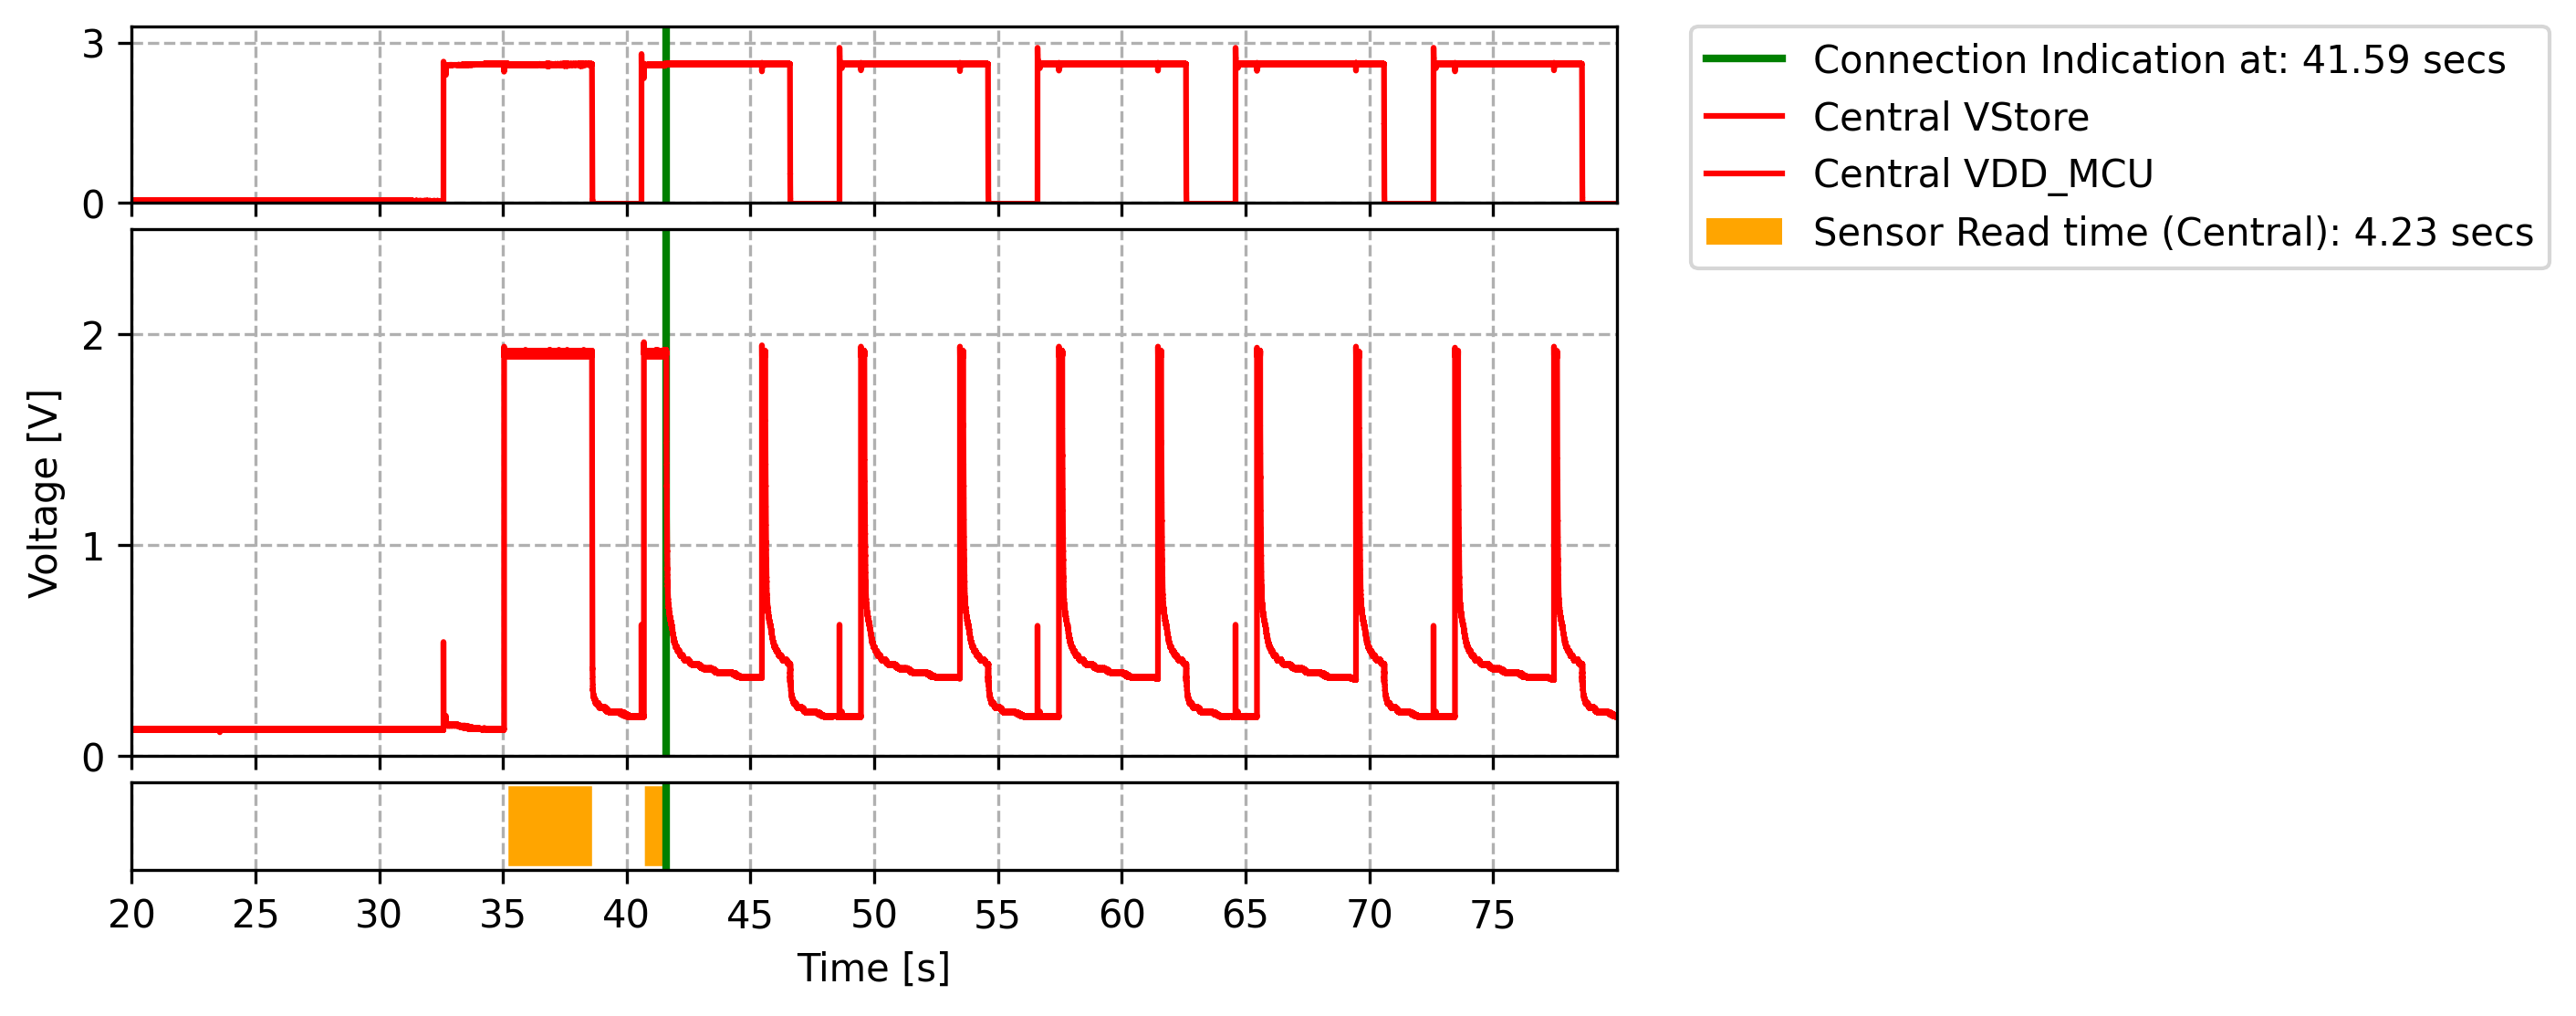
\includegraphics[width=1\linewidth]{chapters/Results/Connection_cardiosync_intermittent_central.png}
        \caption{Voltage measurement for central device.}
        \label{fig:intermittent_connection_cardiosync_central}
    \end{subfigure}
    \caption{Real-time voltage measurement for the CardioSync system \textit{with intermittent power supply}. Each of the three plot in two devices shows different measurement. From the top to bottom in each device, 1) Plot of \(\text{V}_\text{Store}\) : Supply Voltage, 2) Plot of \(\text{V}_\text{DD\_MCU}\) : MCU voltage and 3) Plot of sensor read period indication. The green vertical line through all the plots indicates the successful BLE connection setup event.}
    \label{fig:intermittent_connection_cardiosync}
\end{figure}

\begin{figure}[ht]
    \centering
    \begin{subfigure}{0.85\linewidth}        
        \centering
        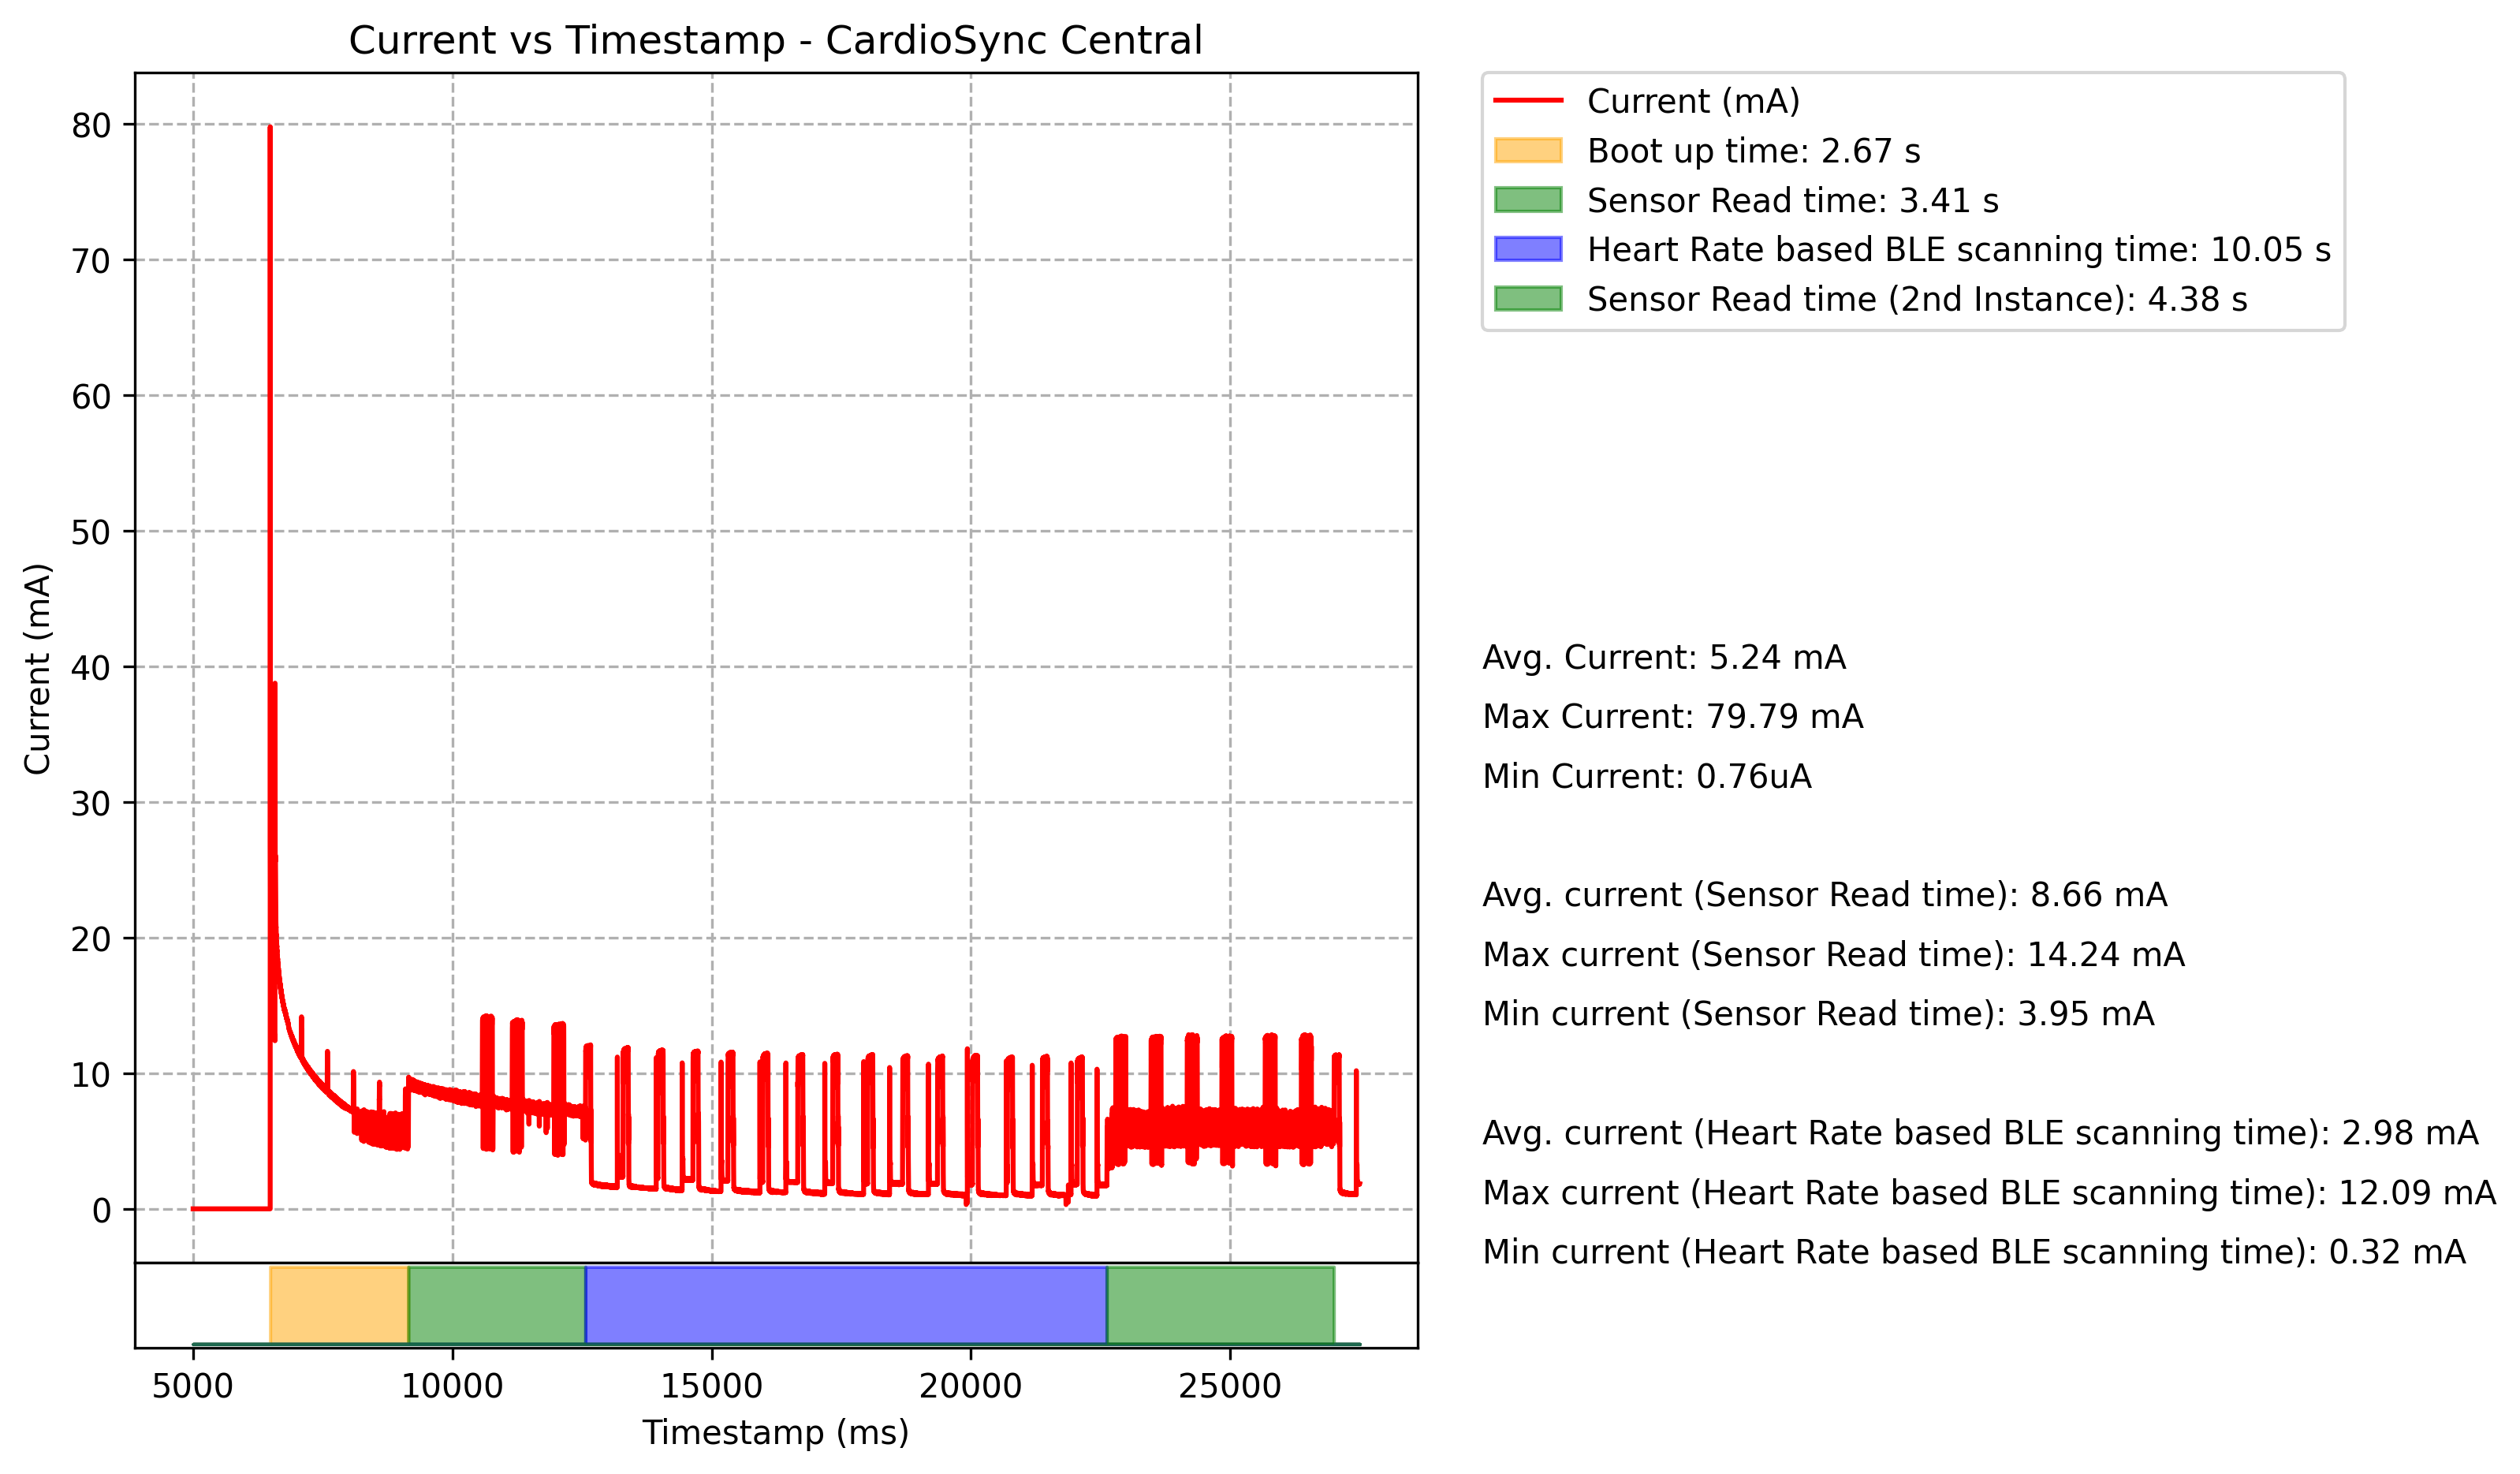
\includegraphics[width=\linewidth]{chapters/Results/Current vs Timestamp - CardioSync Central.png}
        \caption{Central}
        \label{fig:current_cardiosync_central}
    \end{subfigure}
    \begin{subfigure}{0.85\linewidth}    
        \centering
        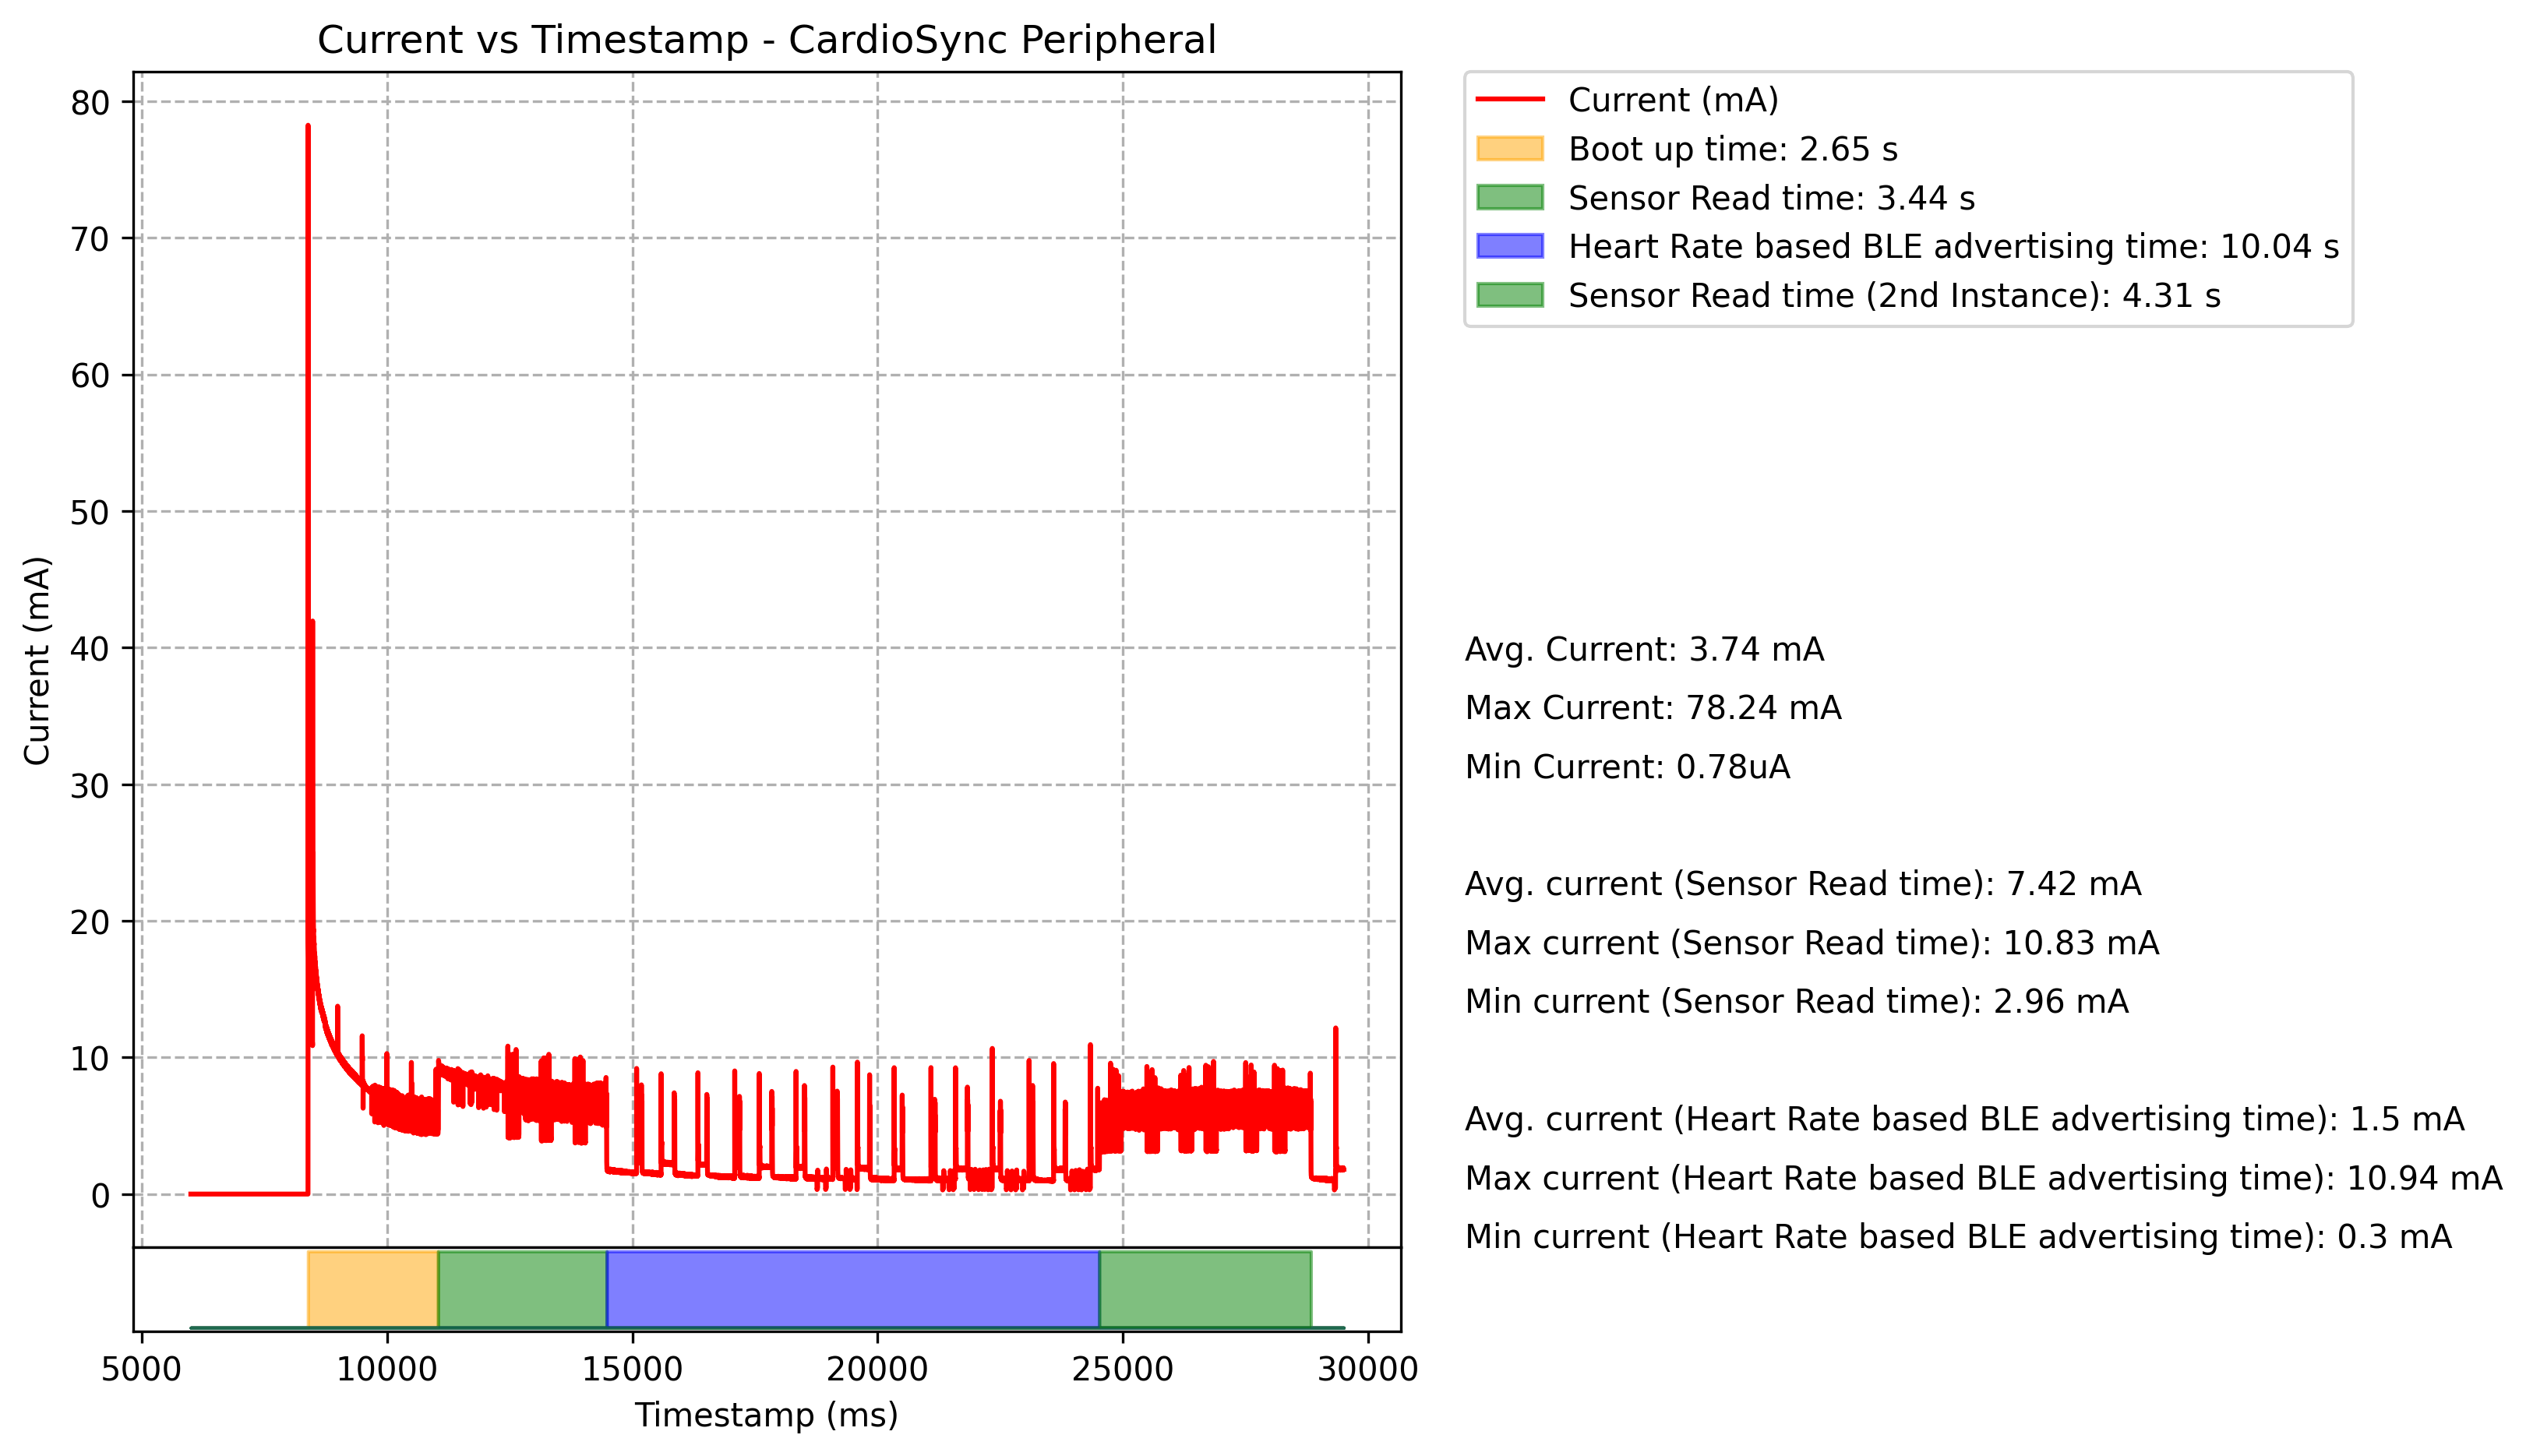
\includegraphics[width=\linewidth]{chapters/Results/Current vs Timestamp - CardioSync Peripheral.png}
        \caption{Peripheral}
        \label{fig:current_cardiosync_peripheral}
    \end{subfigure}
    \caption{Current measurement in idle state without connection establishment for CardioSync systems. Average current consumed in real-time during different phases of the system are differentiated with different colours.}
    \label{fig:current_cardiosync}
\end{figure}

\subsubsection{Validation of Working CardioSync}
The time series plot depicted in \autoref{fig:continous_connection_cardiosync} illustrates the operation of CardioSync framework with continuous powered input. It can be asserted from the plot that there is the periodic shutdown of \(\text{V}_\text{DD\_MCU}\) during times of inactivity, therefore corroborating the anticipated power-saving benefits associated with the integration of FreeBie.
\vspace{1\baselineskip}

\noindent As elucidated in Chapter \ref{chap:implementation}, the system from \autoref{fig:continous_connection_cardiosync} demonstrates the anticipated functionality of "Read and Synchronise" for a period of \textit{3.40 seconds} where the sensor is being actively read. Followed by that, we also see  the "Sleep and Synchronise" functionality, where the system exclusively reactivates at the interval of each heartbeat pulse in order to initiate a connection. The connection establishment event, which is closely synced with the heart rate pulses, is shown by the green vertical line in Figure \ref{fig:continous_connection_cardiosync}.
\vspace{1\baselineskip}

\noindent A similar verification was conducted under intermittent power supply using a square wave signal with a duty cycle of 75\% for a duration of 8 seconds. The time series plot (\autoref{fig:intermittent_connection_cardiosync}) reveals the system's adaptability to changing power availability, as connections continue to be established in coordination with the heart beat, despite power fluctuations. In addition, the CardioSync system was tested across various square wave periods with different duty cycles as shown in Table \ref{tab:cardiosync_intermittent_exp} in Appendix \ref{app:appendix_a}, demonstrating its adaptability to different supply configurations.

\subsubsection{Current Measurement of CardioSync system}
Figure \ref{fig:current_cardiosync}, gives us the current measurement for different phases of the CardioSync system operation for synchronising BLE connection. The measured current values are afterwards utilised for comparative analysis against naive reference system.
\vspace{1\baselineskip}

\noindent It is important to note that the "Read and Synchronise" phase requires a higher current compared to the "Sleep and Synchronise" phase. This behaviour is substantiated across both central and peripheral devices in the current measurement-driven evaluation. In the Central device, "Read and Synchronise" phase happens for around \textit{3.41 seconds} and consumes an average current of approximately \textit{8.66mA}. Similarly, the Peripheral device registers \textit{7.42mA} over a \textit{3.44-second} interval of sensor read phase. Notably, during the "Sleep and Synchronise" phase of 10 seconds, both central and peripheral devices exhibit a substantially lower average current consumption—\textit{2.98mA and 1.5mA}, respectively.
\vspace{1\baselineskip}

\noindent The values of these evaluation are afterwards utilised in the computation of the energy expended by the device for the purpose of synchronising a BLE connection.


\section{Comparative Analysis against Naive Reference Design}
In this section, we start by introducing a naive reference model of Battery-Free BLE. This model will be used as a yardstick to gauge the effectiveness of our synchronised CardioSync system.

\subsection{Naive Reference FreeBie Model}

\noindent To ensure a comprehensive comparison, the reference system used is the FreeBie system, which lacks any synchronisation method. For experimental purposes, both the Central and Peripheral components of the FreeBie reference model were intentionally set to have matching Advertising and Scanning intervals, preventing any permanent link failure.
\vspace{1\baselineskip}

\begin{table}[t]
\centering
\begin{tabular}{|c|cc|}
\hline
\textbf{\begin{tabular}[c]{@{}c@{}}Configuration\\ Name\end{tabular}} & \multicolumn{2}{c|}{\textbf{\begin{tabular}[c]{@{}c@{}}Configured BLE\\ parameters\end{tabular}}} \\ \hline
\cellcolor[HTML]{32CB00} & \multicolumn{1}{c|}{\textit{\begin{tabular}[c]{@{}c@{}}Advertising\\ Interval\end{tabular}}} & 6 seconds        \\ \cline{2-3} 
\cellcolor[HTML]{32CB00} & \multicolumn{1}{c|}{\textit{\begin{tabular}[c]{@{}c@{}}Scanning\\ Interval\end{tabular}}}    & 6 seconds        \\ \cline{2-3} 
\multirow{-3}{*}{\cellcolor[HTML]{32CB00}\textbf{Low}}    & \multicolumn{1}{c|}{\textit{\begin{tabular}[c]{@{}c@{}}Scanning\\ Window\end{tabular}}} & 1 second         \\ \hline
\cellcolor[HTML]{FFCB2F} & \multicolumn{1}{c|}{\textit{\begin{tabular}[c]{@{}c@{}}Advertising\\ Interval\end{tabular}}} & 2 seconds        \\ \cline{2-3} 
\cellcolor[HTML]{FFCB2F} & \multicolumn{1}{c|}{\textit{\begin{tabular}[c]{@{}c@{}}Scanning\\ Interval\end{tabular}}}    & 2 seconds        \\ \cline{2-3} 
\multirow{-3}{*}{\cellcolor[HTML]{FFCB2F}\textbf{Medium}} & \multicolumn{1}{c|}{\textit{\begin{tabular}[c]{@{}c@{}}Scanning\\ Window\end{tabular}}} & 500 milliseconds \\ \hline
\cellcolor[HTML]{FD6864} & \multicolumn{1}{c|}{\textit{\begin{tabular}[c]{@{}c@{}}Advertising\\ Interval\end{tabular}}} & 500 milliseconds \\ \cline{2-3} 
\cellcolor[HTML]{FD6864} & \multicolumn{1}{c|}{\textit{\begin{tabular}[c]{@{}c@{}}Scanning\\ Interval\end{tabular}}}    & 500 milliseconds \\ \cline{2-3} 
\multirow{-3}{*}{\cellcolor[HTML]{FD6864}\textbf{High}}  & \multicolumn{1}{c|}{\textit{\begin{tabular}[c]{@{}c@{}}Scanning\\ Window\end{tabular}}} & 125 milliseconds \\ \hline
\end{tabular}
\caption{Chosen BLE parameters for Reference FreeBie system}
\label{tab:ble_params_freebie}
\end{table}

\noindent To enrich our data pool, we selected three distinct BLE configurations for the FreeBie system, each characterised by varying energy consumption, as detailed in \autoref{tab:ble_params_freebie}. To provide practical real-world context, each configuration represents a scenario within the realm of body sensor networks. These diverse scenarios provide a practical basis for comparing the performance of the CardioSync framework with the reference FreeBie system.

\begin{itemize}
    \item \textbf{FreeBie Low (Limited-Energy Scenario):} This scenario envisions a wearable sensor attached to a person's shoe sole, relying on minimal energy generated through piezoelectric energy harvesting from each step. In this challenging environment, efficient energy management during connection attempts is crucial.
    
    \item \textbf{FreeBie Medium (Balanced-Energy Scenario):} In this scenario, the device is part of a fitness tracker, like a wristband, accessing moderate energy from a solar cells. While energy constraints are less severe than in the Low scenario, efficient energy use remains vital.
    
    \item \textbf{FreeBie High (Abundant-Energy Scenario):} Two energy sources are considered, one on the wrist and one on the ankle, harnessing abundant energy from solar cells and motion harvesting, respectively. These devices can expend energy liberally for frequent connection attempts, emphasising connection efficiency.
\end{itemize}


\begin{figure}[t]
    \begin{subfigure}{0.5\linewidth}
        \centering
        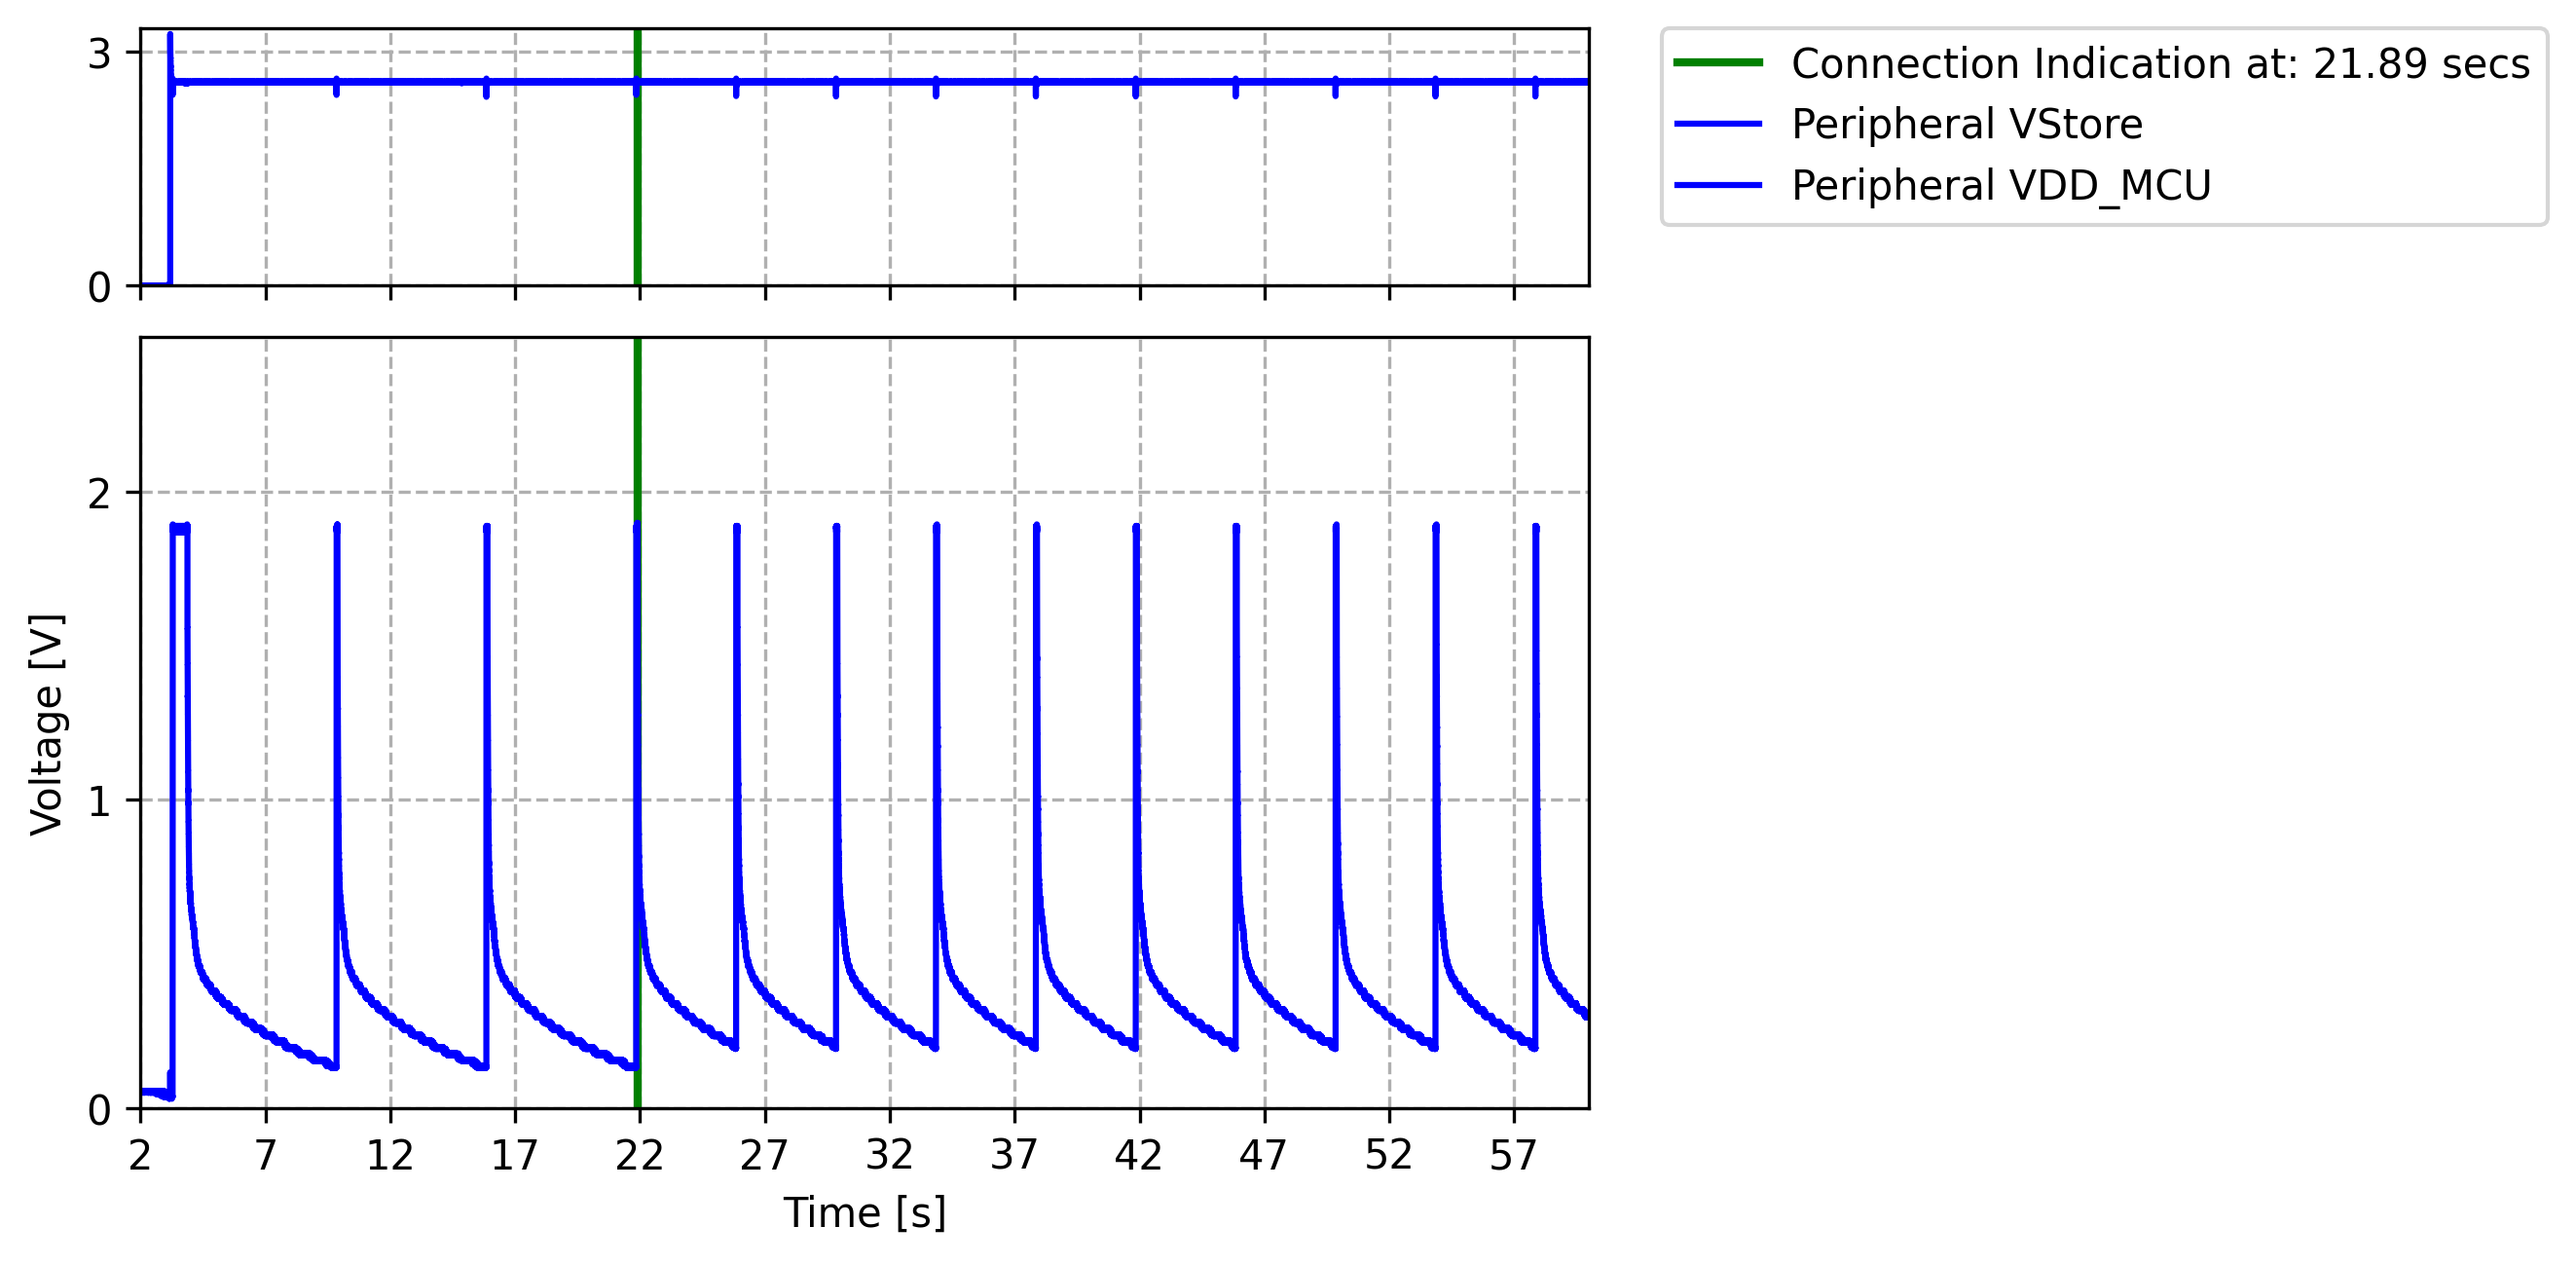
\includegraphics[width=1\linewidth]{chapters/Results/Connection_Freebie_low_peripheral.png}
        \caption{\scriptsize{FreeBie Low - Peripheral}}
        \vspace{1\baselineskip}
    \end{subfigure}\hfill
    \begin{subfigure}{0.5\linewidth}
        \centering
        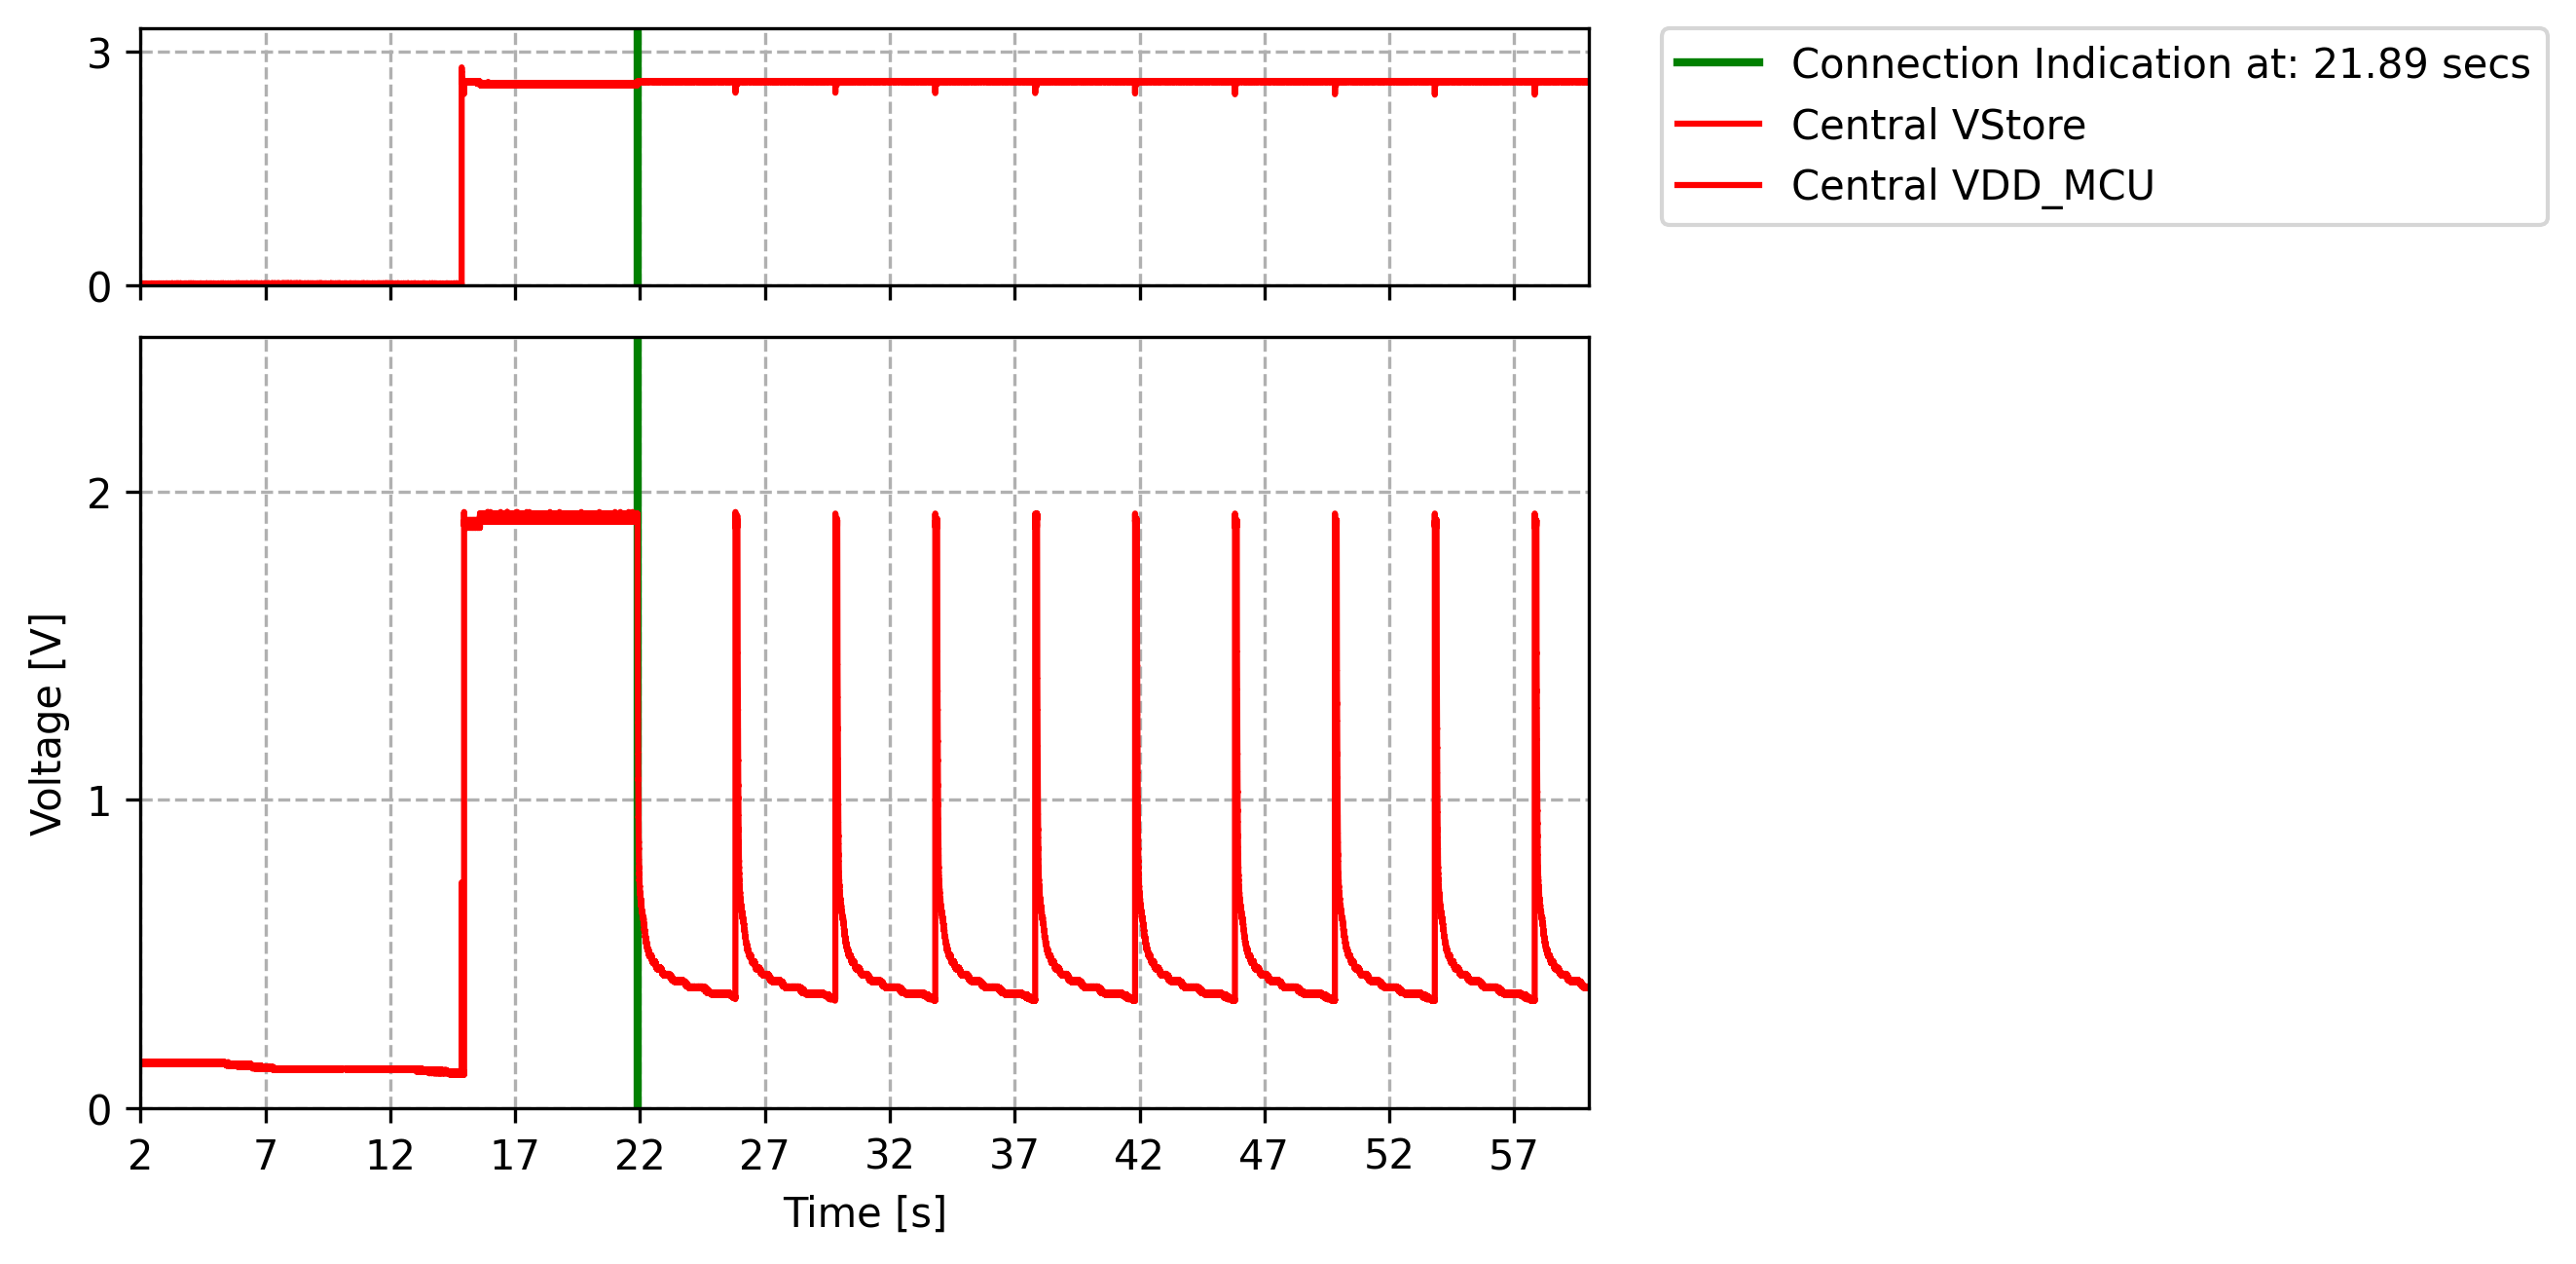
\includegraphics[width=1\linewidth]{chapters/Results/Connection_Freebie_low_central.png}
        \caption{\scriptsize{FreeBie Low - Central}}
        \vspace{1\baselineskip}
    \end{subfigure}
    \begin{subfigure}{0.5\linewidth}
        \centering
        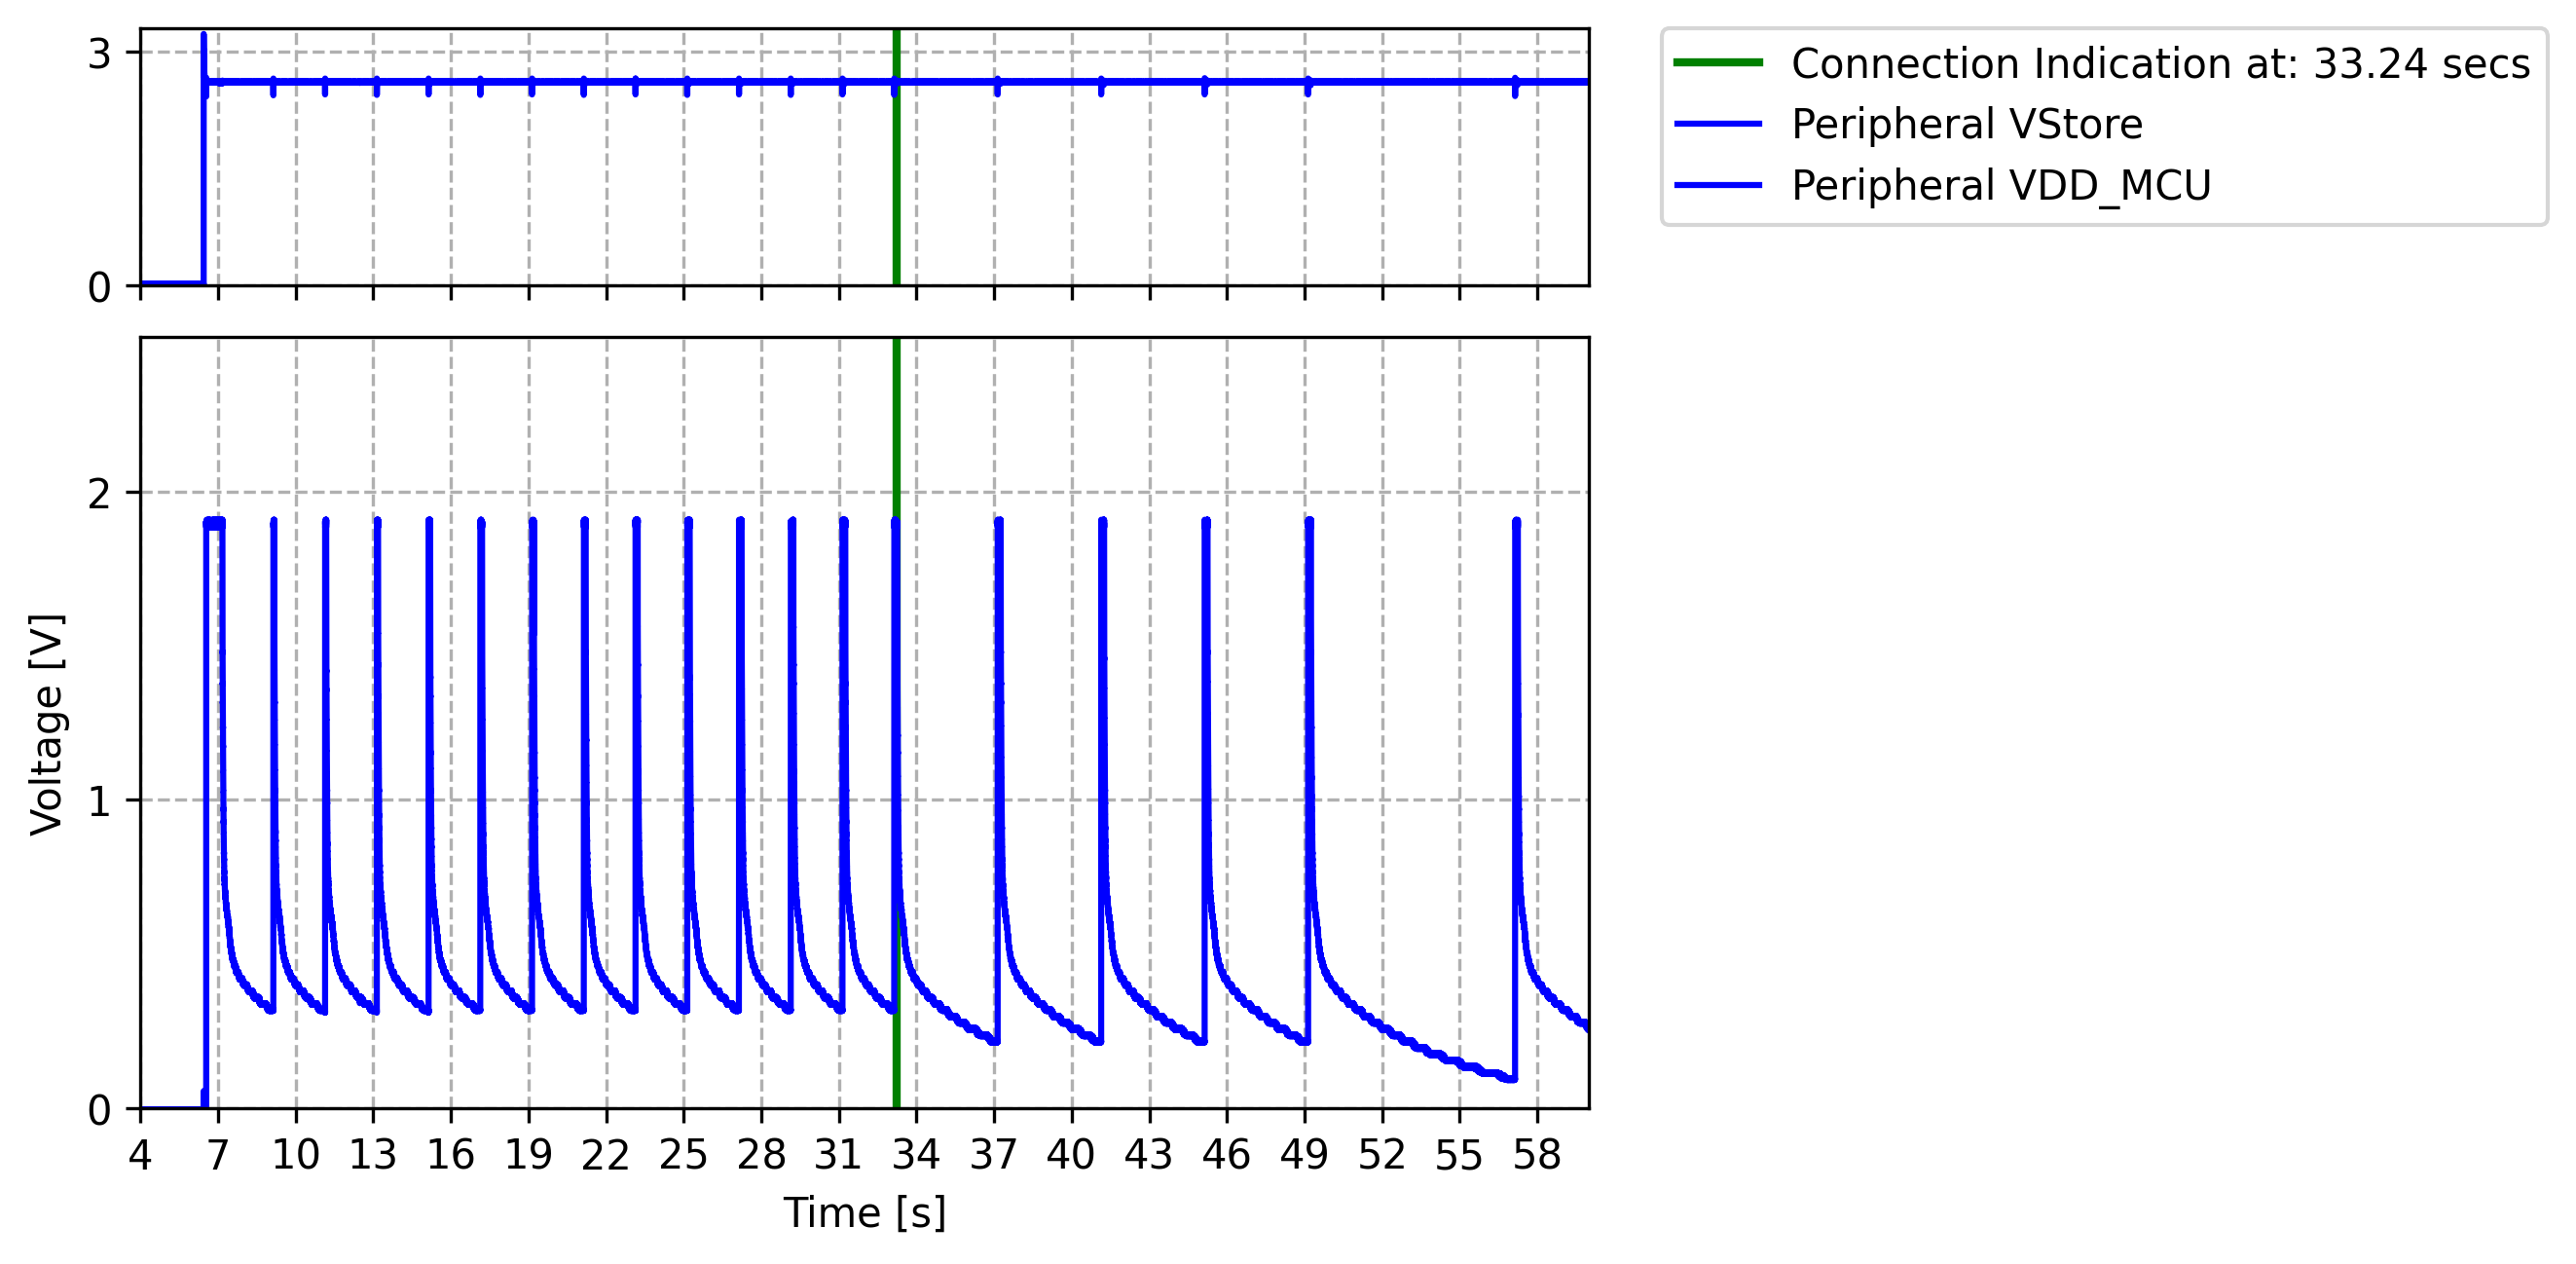
\includegraphics[width=1\linewidth]{chapters/Results/Connection_Freebie_medium_peripheral.png}
        \caption{\scriptsize{FreeBie Medium - Peripheral}}
        \vspace{1\baselineskip}
    \end{subfigure}\hfill
    \begin{subfigure}{0.5\linewidth}
        \centering
        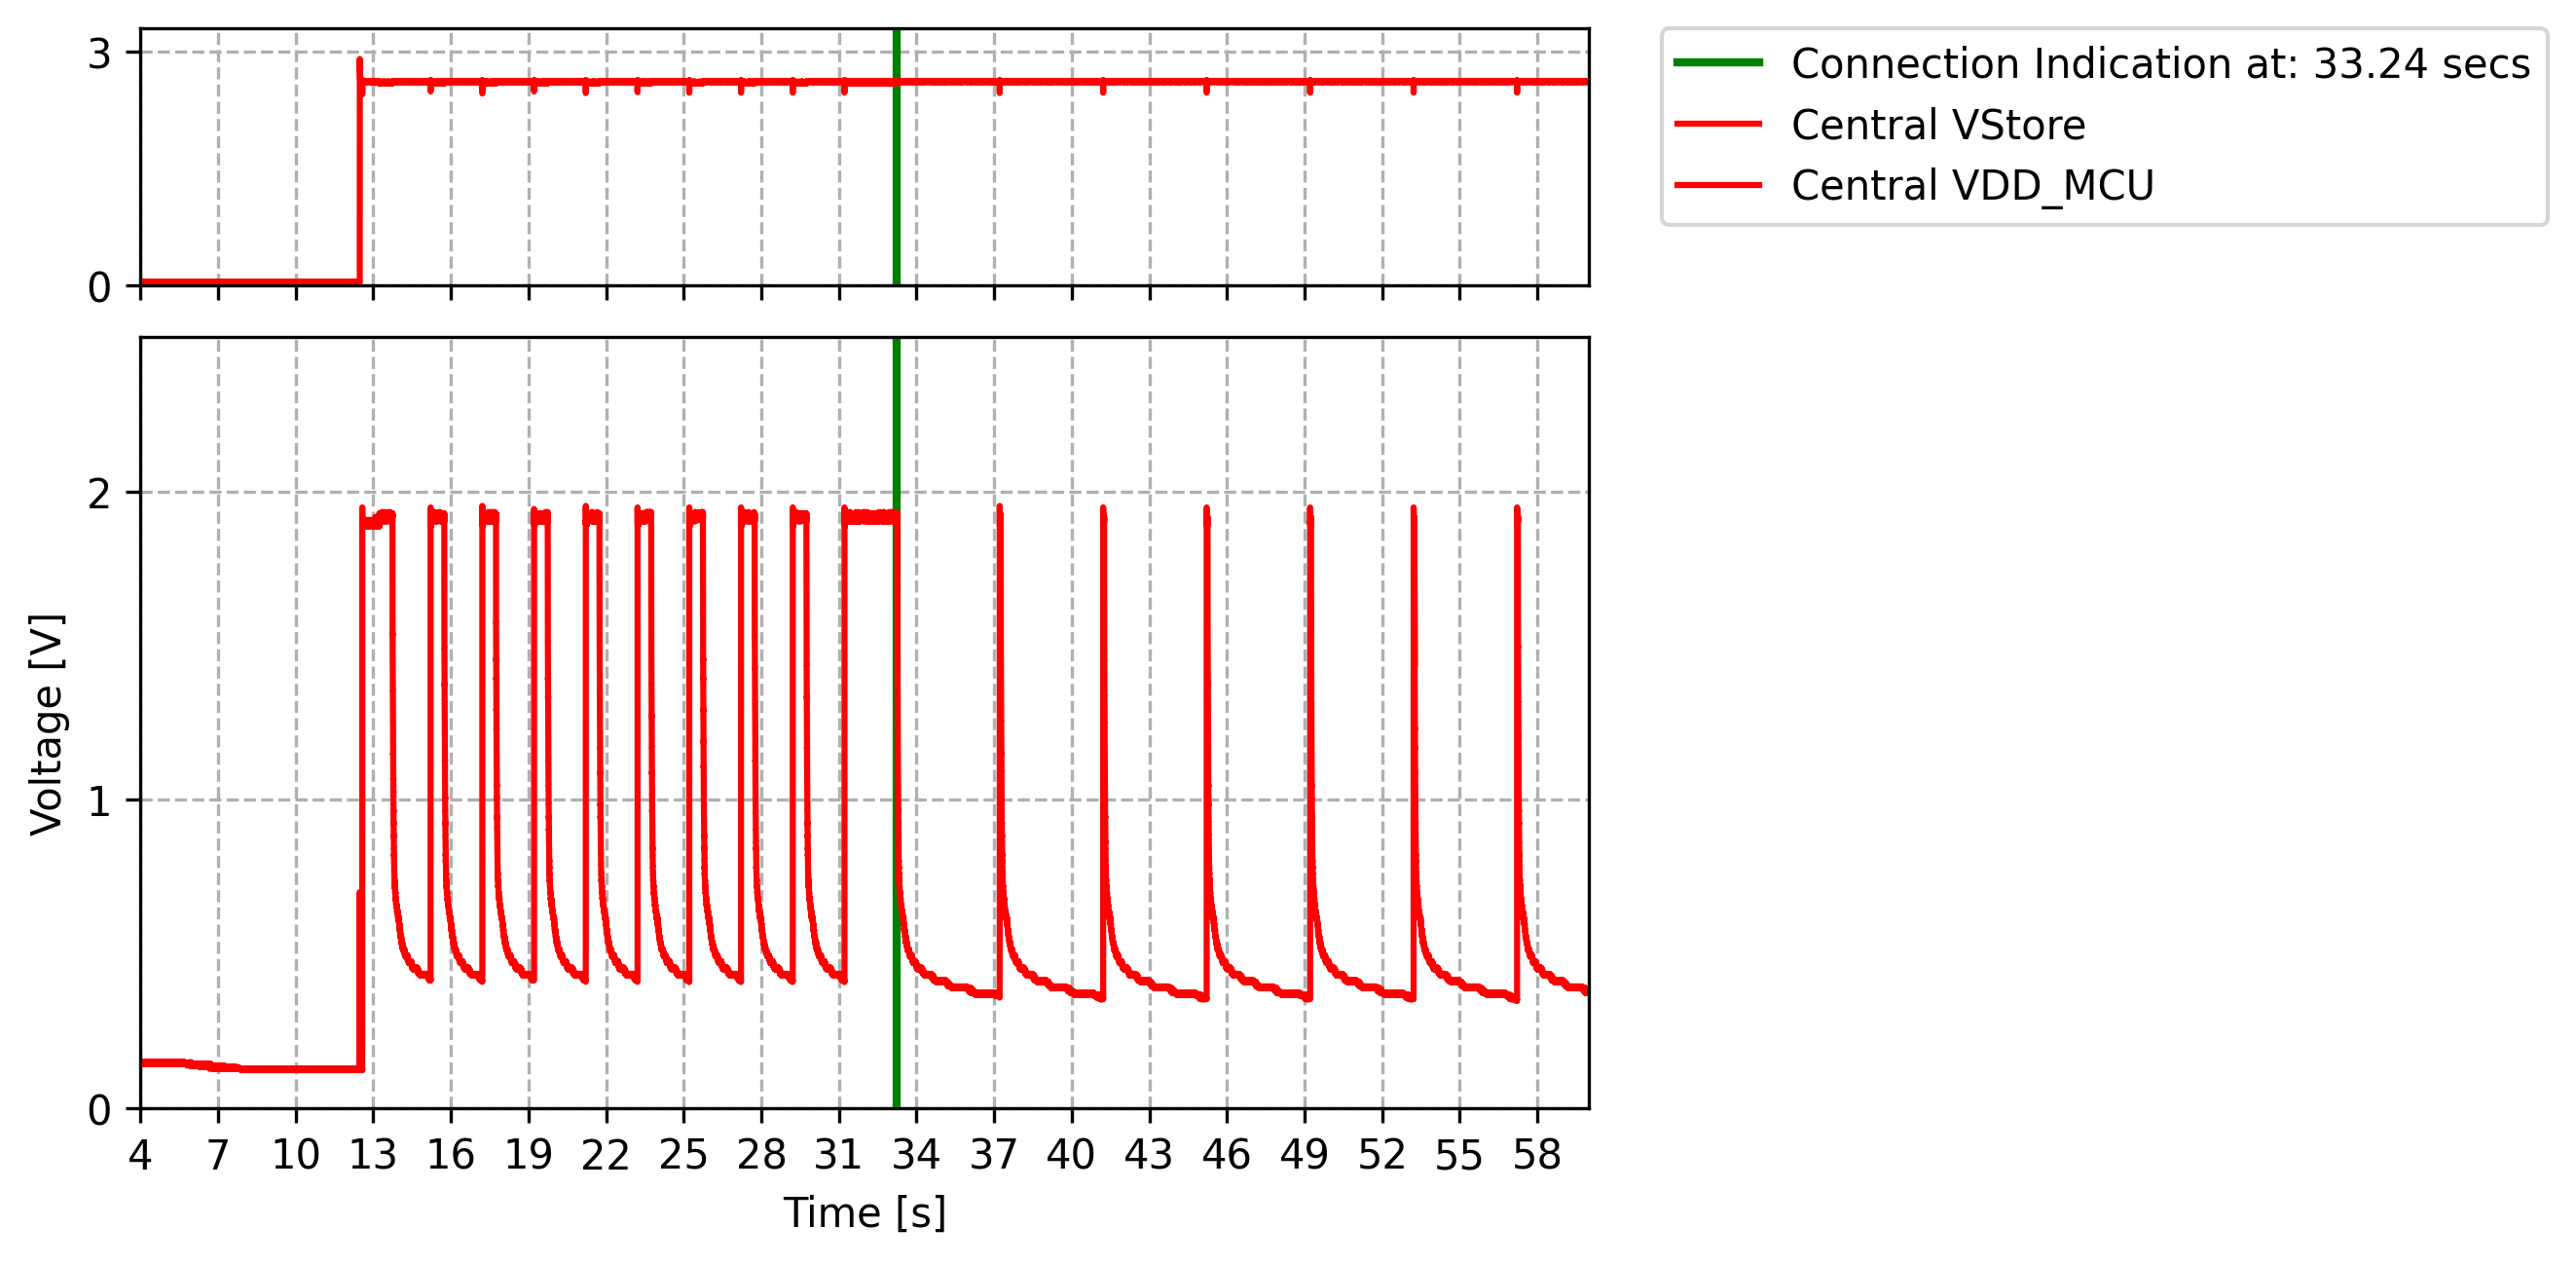
\includegraphics[width=1\linewidth]{chapters/Results/Connection_Freebie_medium_central.png}
        \caption{\scriptsize{FreeBie Medium - Central}}
        \vspace{1\baselineskip}
    \end{subfigure}
    \begin{subfigure}{0.5\linewidth}
        \centering
        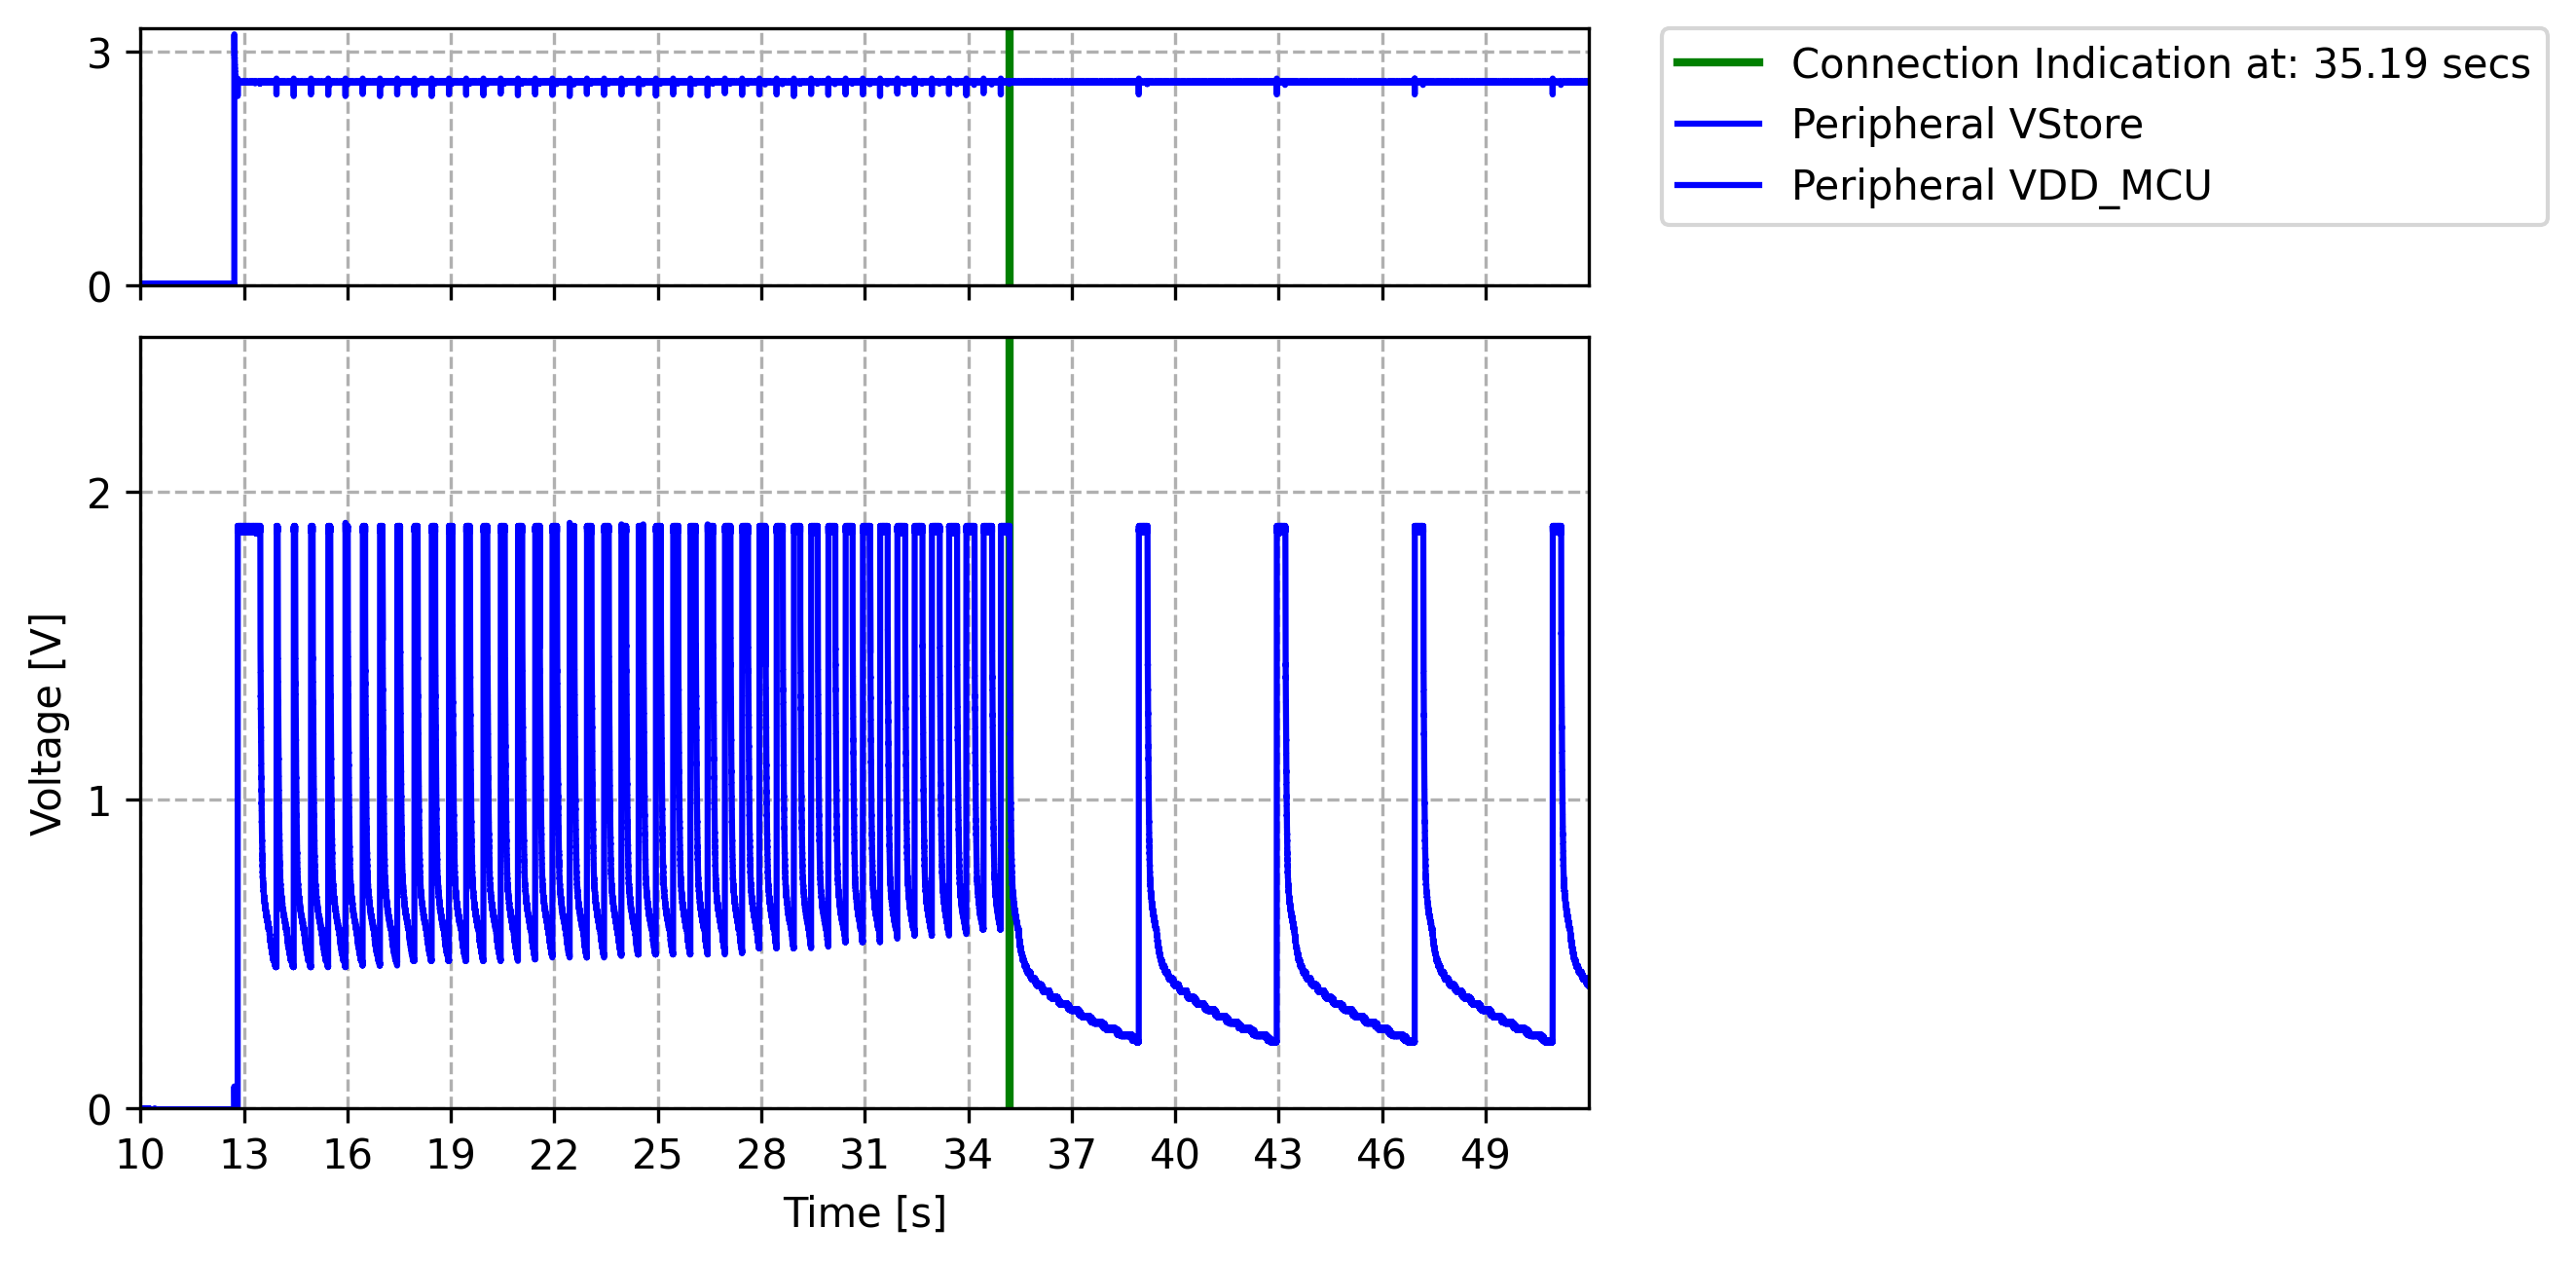
\includegraphics[width=1\linewidth]{chapters/Results/Connection_Freebie_high_peripheral.png}
        \caption{\scriptsize{FreeBie High - Peripheral}}
    \end{subfigure} \hfill
    \begin{subfigure}{0.5\linewidth}
        \centering
        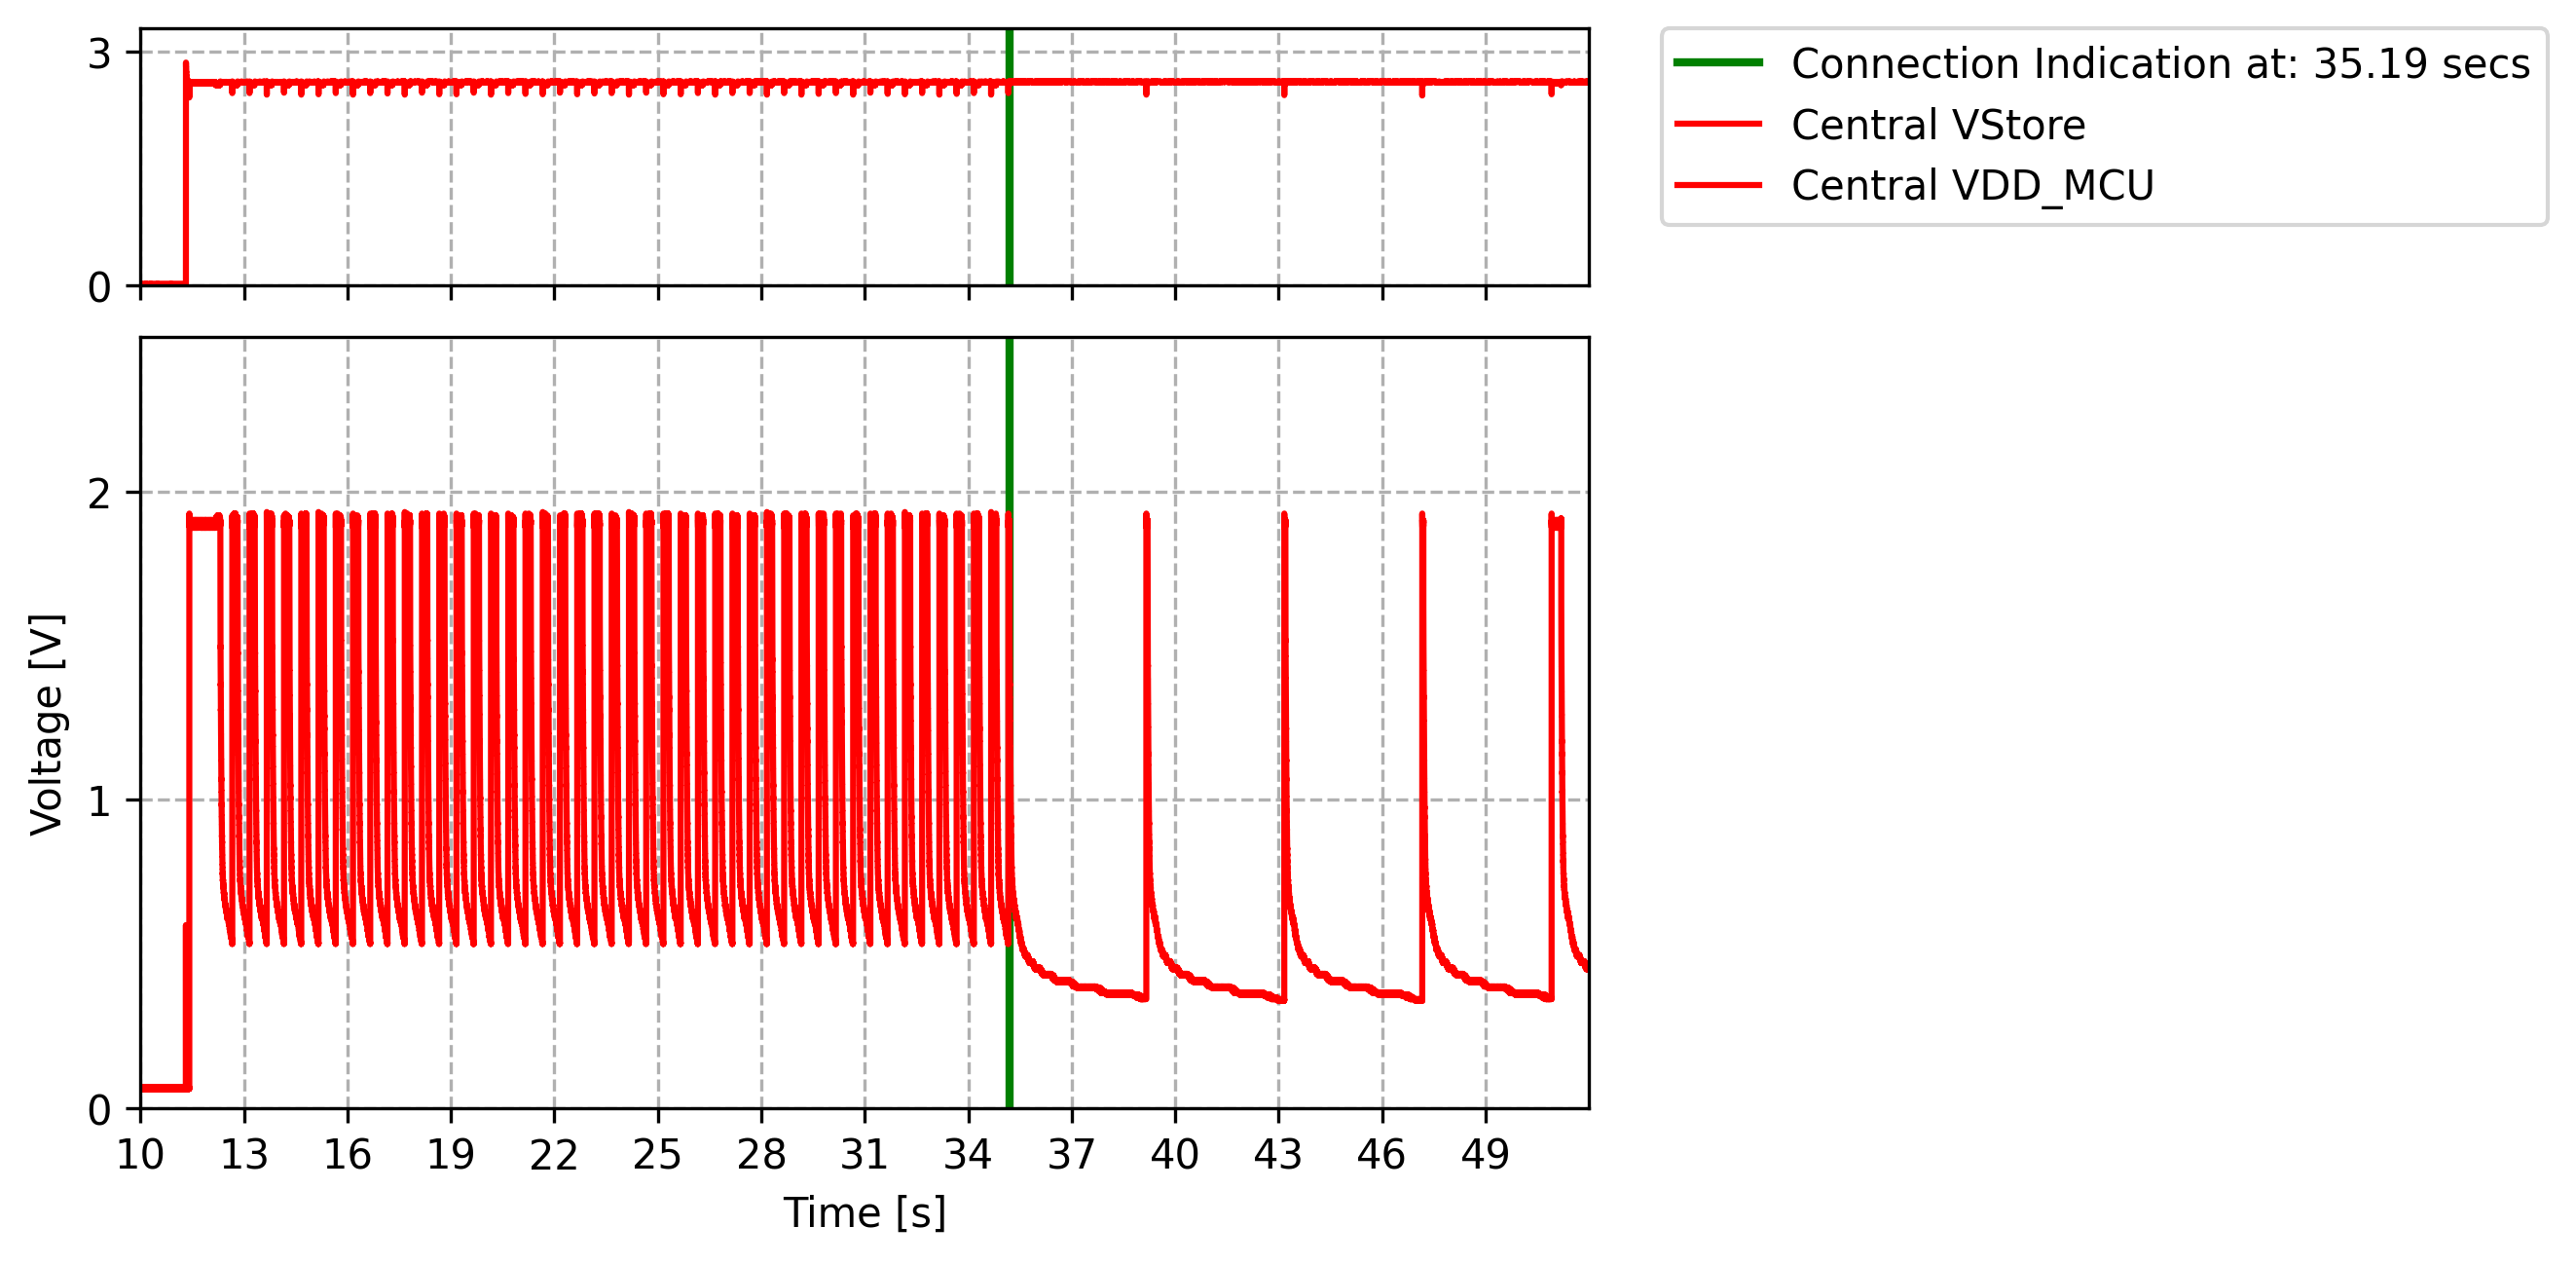
\includegraphics[width=1\linewidth]{chapters/Results/Connection_Freebie_high_central.png}
        \caption{\scriptsize{FreeBie High - Central device}}
    \end{subfigure}         
    \caption{Real-time voltage measurement of FreeBie system. Each of the two plots in both devices for each configuration shows different measurements. From top to bottom in each device, 1) Plot of \(\text{V}_\text{Store}\) : Supply Voltage and 2) Plot of \(\text{V}_\text{DD\_MCU}\) : MCU voltage. The green vertical line through all the plots indicates the successful BLE connection setup event.}
    \label{fig:voltage_freebie}
\end{figure}
\begin{figure}[t]
    \begin{subfigure}{0.45\linewidth}
        \centering
        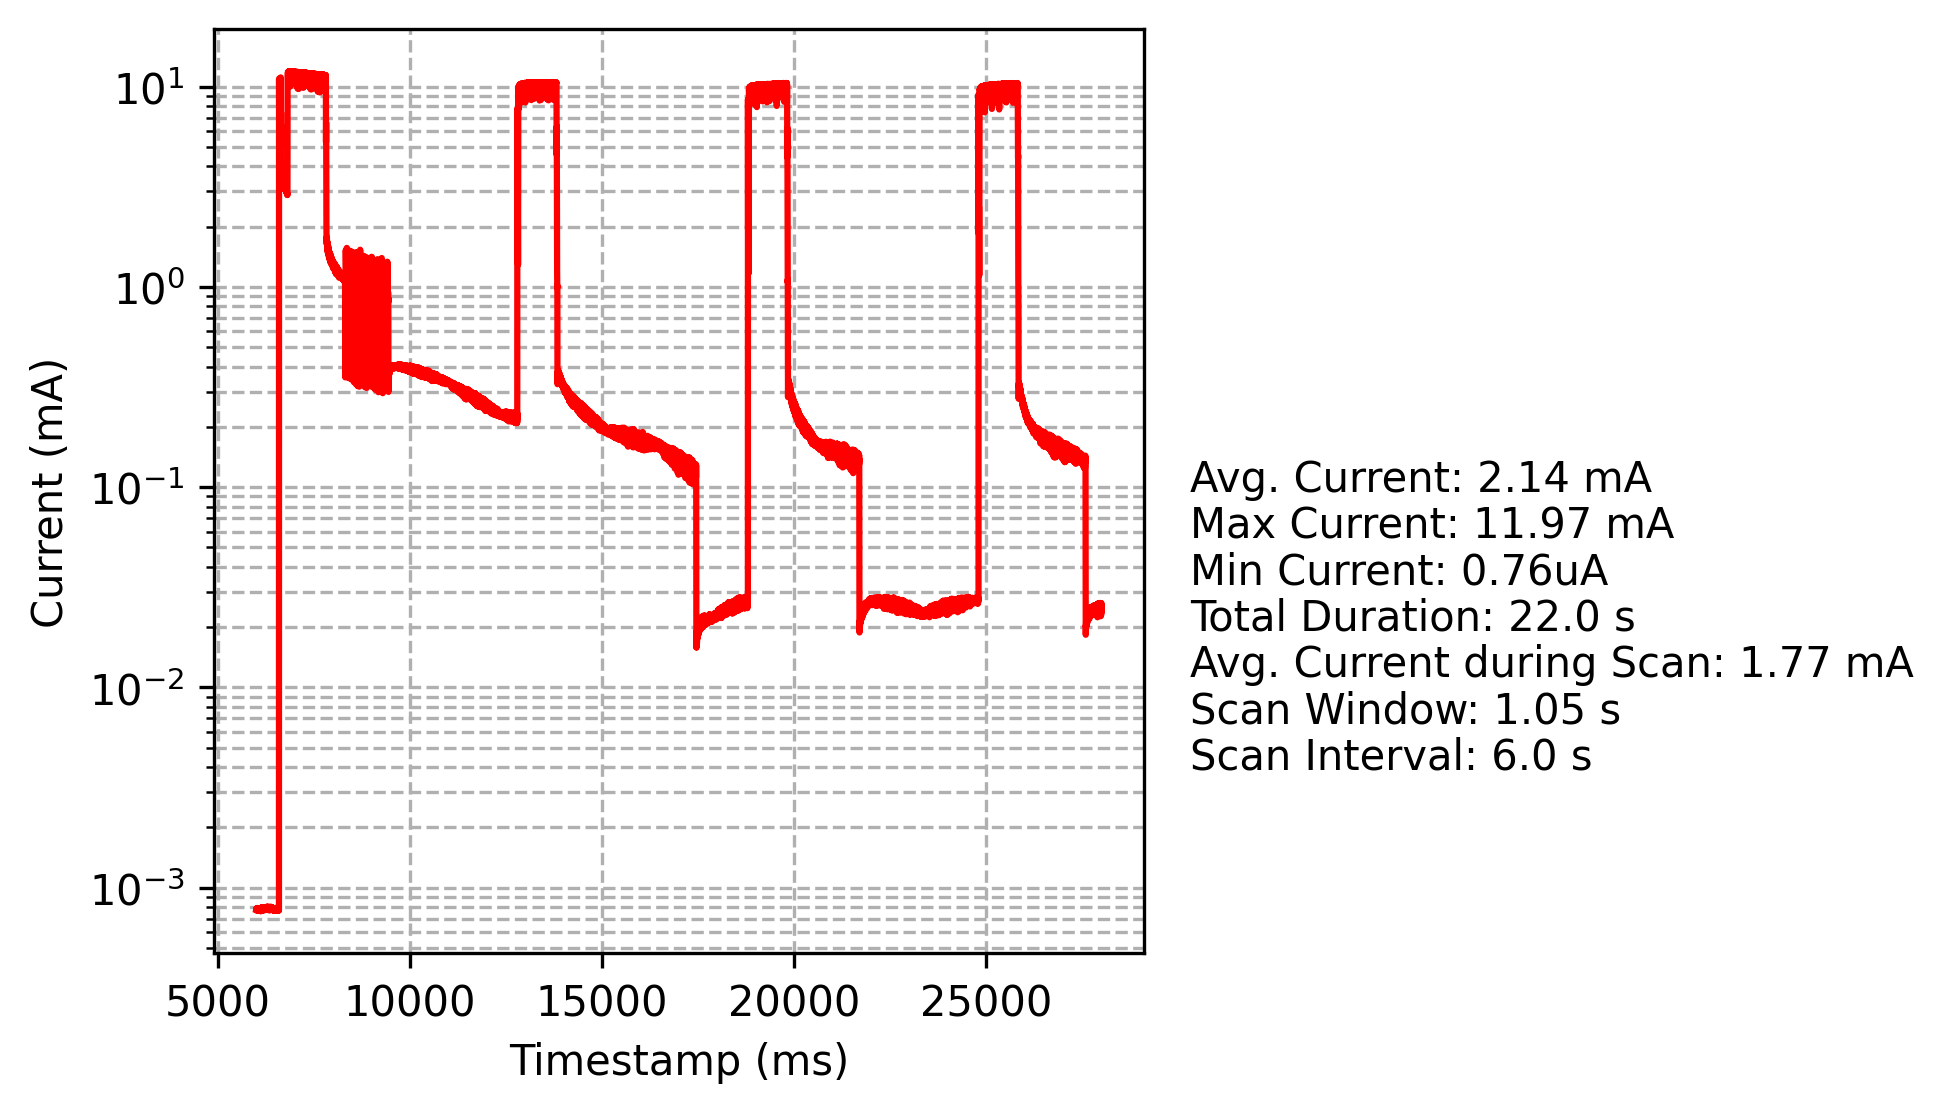
\includegraphics[width=\linewidth]{chapters/Results/Current vs Timestamp - FreeBie Central Low.png}
        \caption{FreeBie Low - Central}
        \label{fig:freebie_low_central}
    \end{subfigure}\hfill
    \begin{subfigure}{0.45\linewidth}
        \centering
        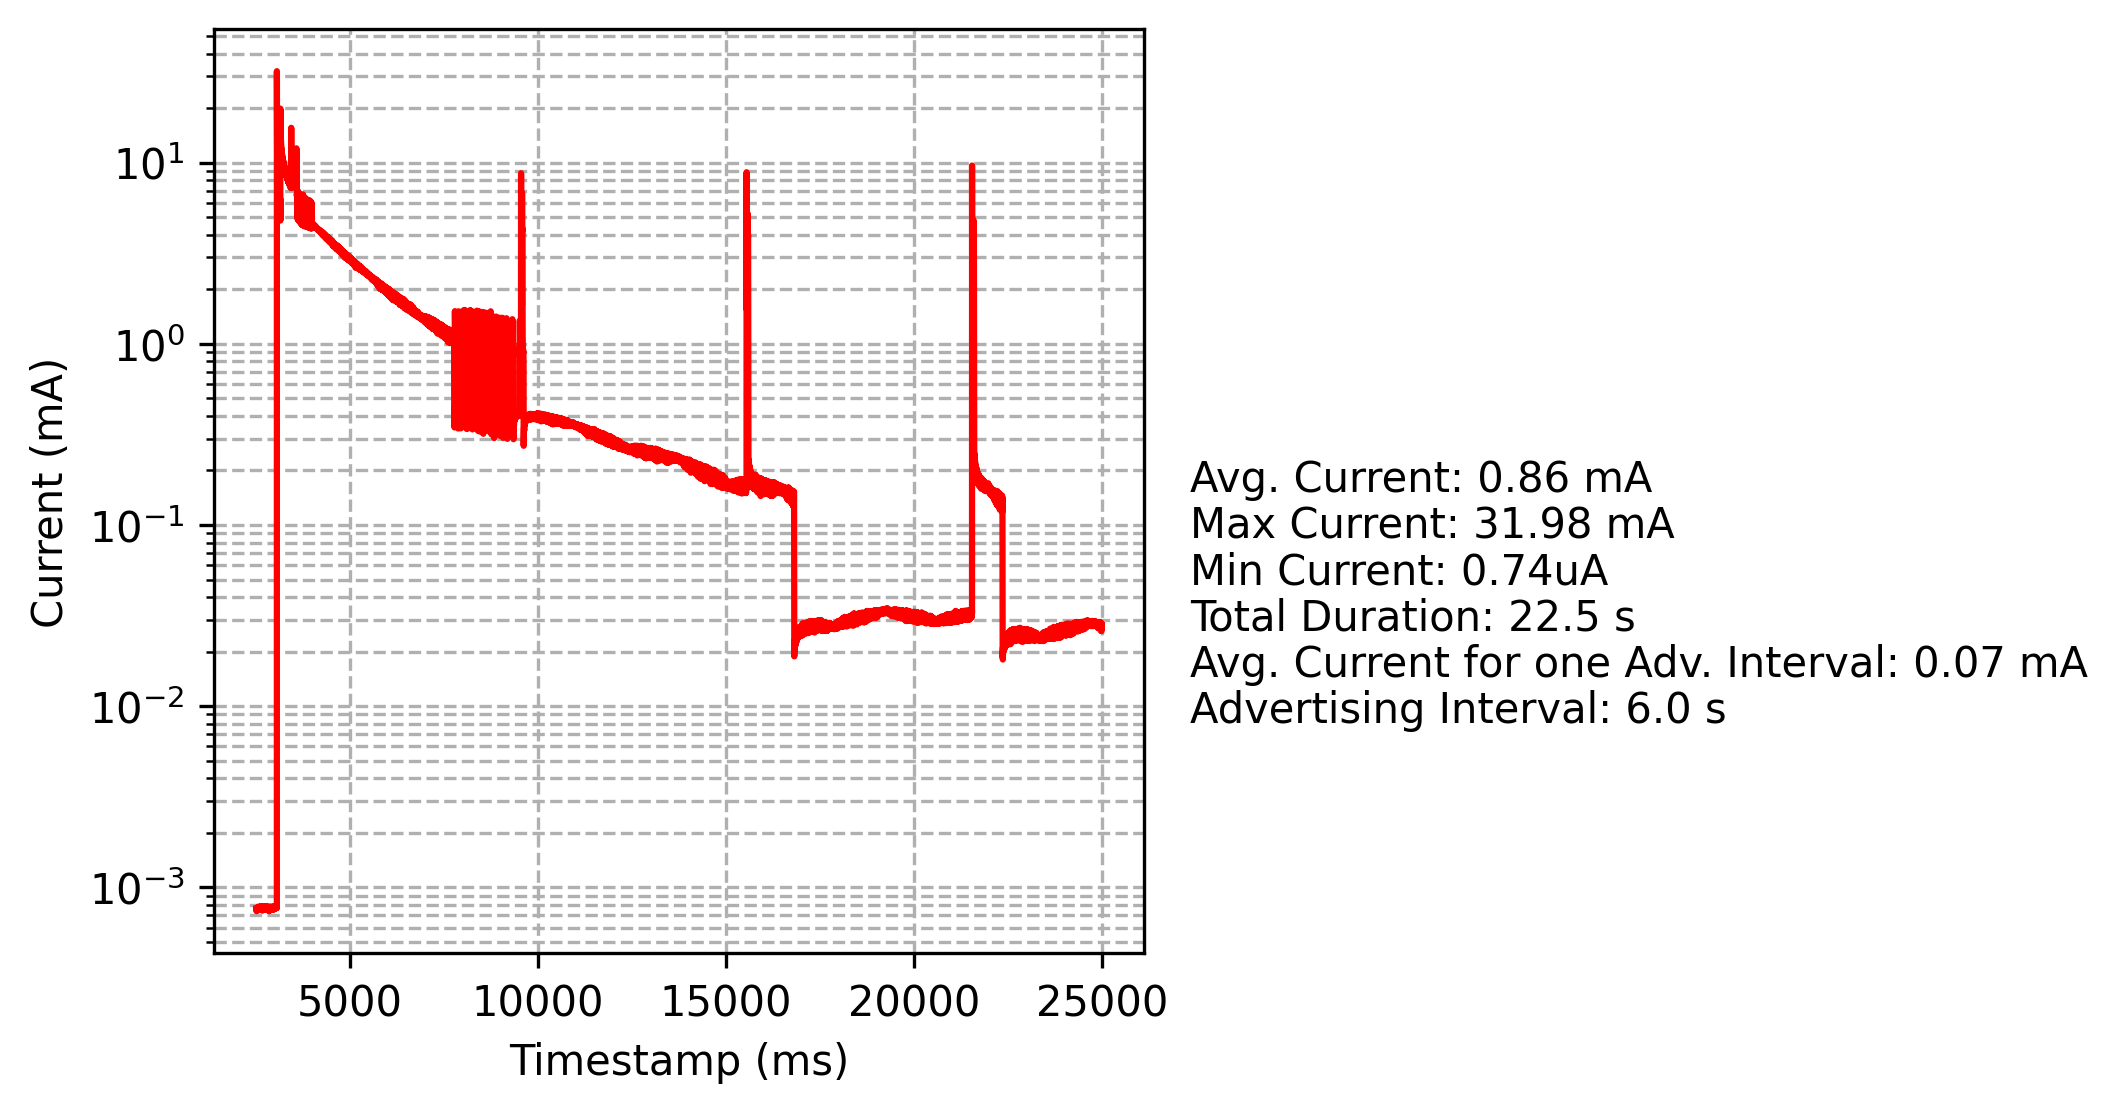
\includegraphics[width=\linewidth]{chapters/Results/Current vs Timestamp - FreeBie Peripheral Low.png}
        \caption{FreeBie Low - Peripheral}
        \label{fig:freebie_low_peripheral}
    \end{subfigure}
    \begin{subfigure}{0.45\linewidth}
        \centering
        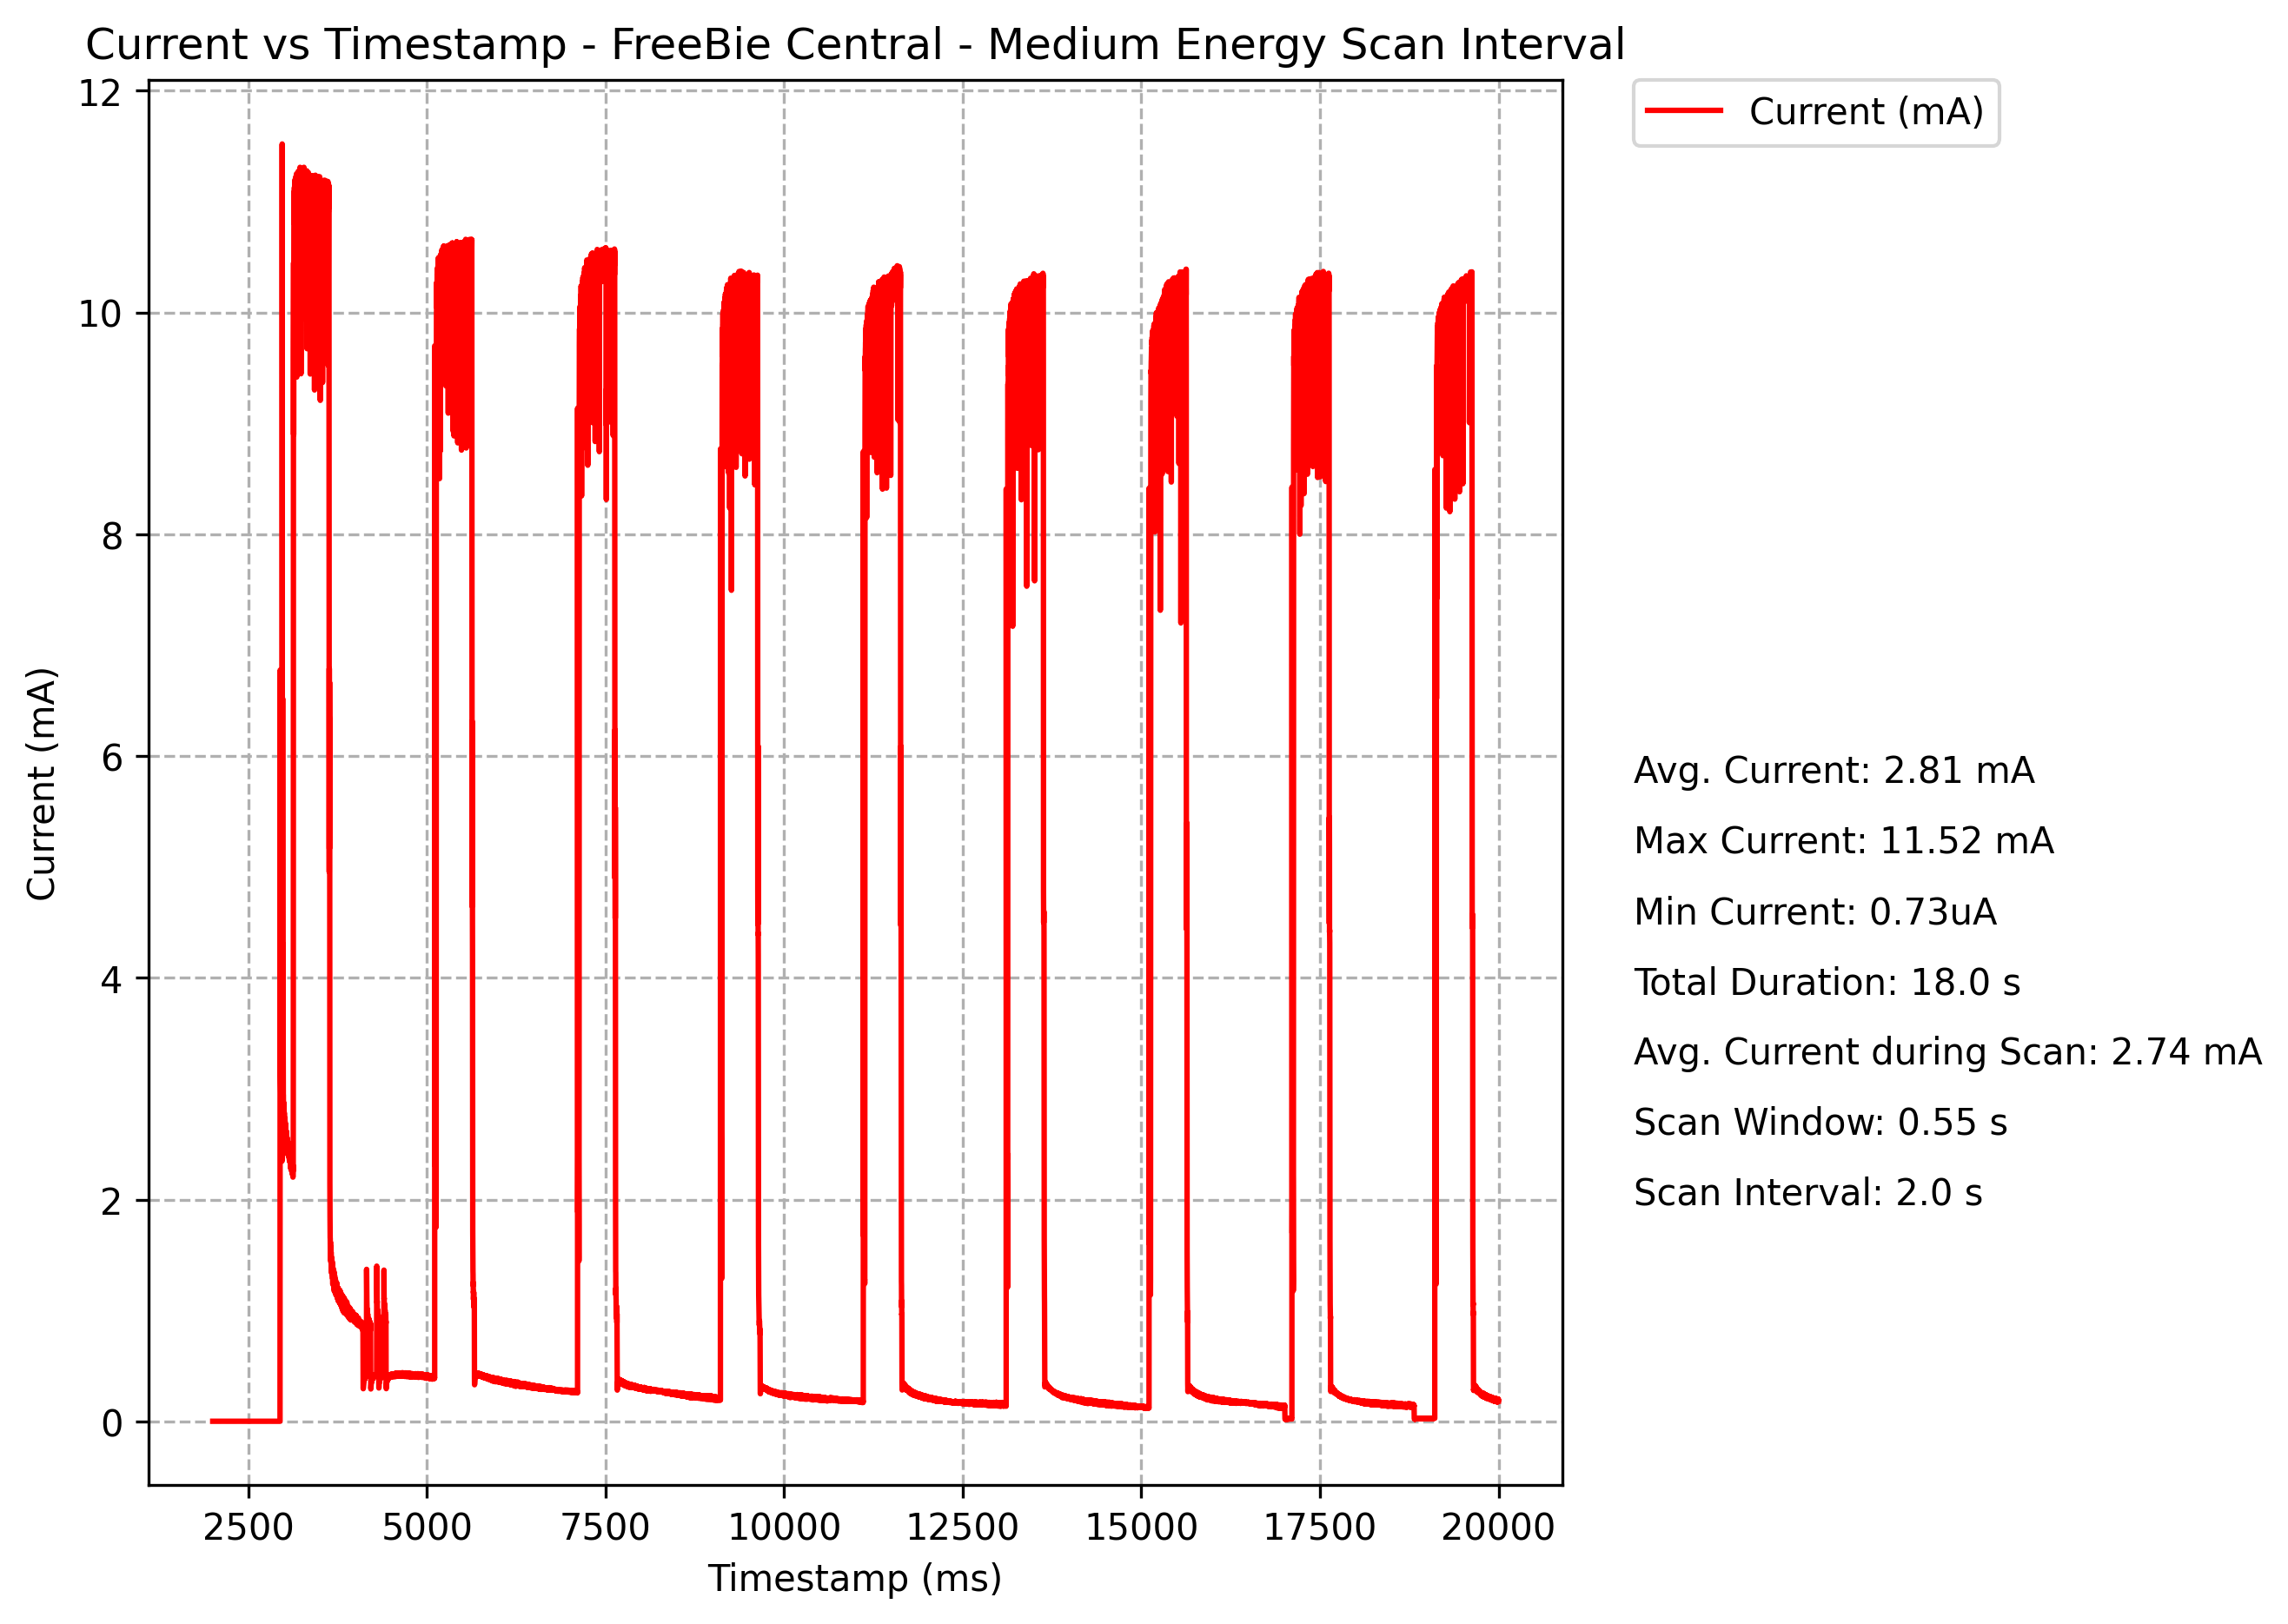
\includegraphics[width=\linewidth]{chapters/Results/Current vs Timestamp - FreeBie Central Medium.png}
        \caption{FreeBie Medium- Central}
        \label{fig:freebie_medium_central}
    \end{subfigure}\hfill
    \begin{subfigure}{0.45\linewidth}
        \centering
        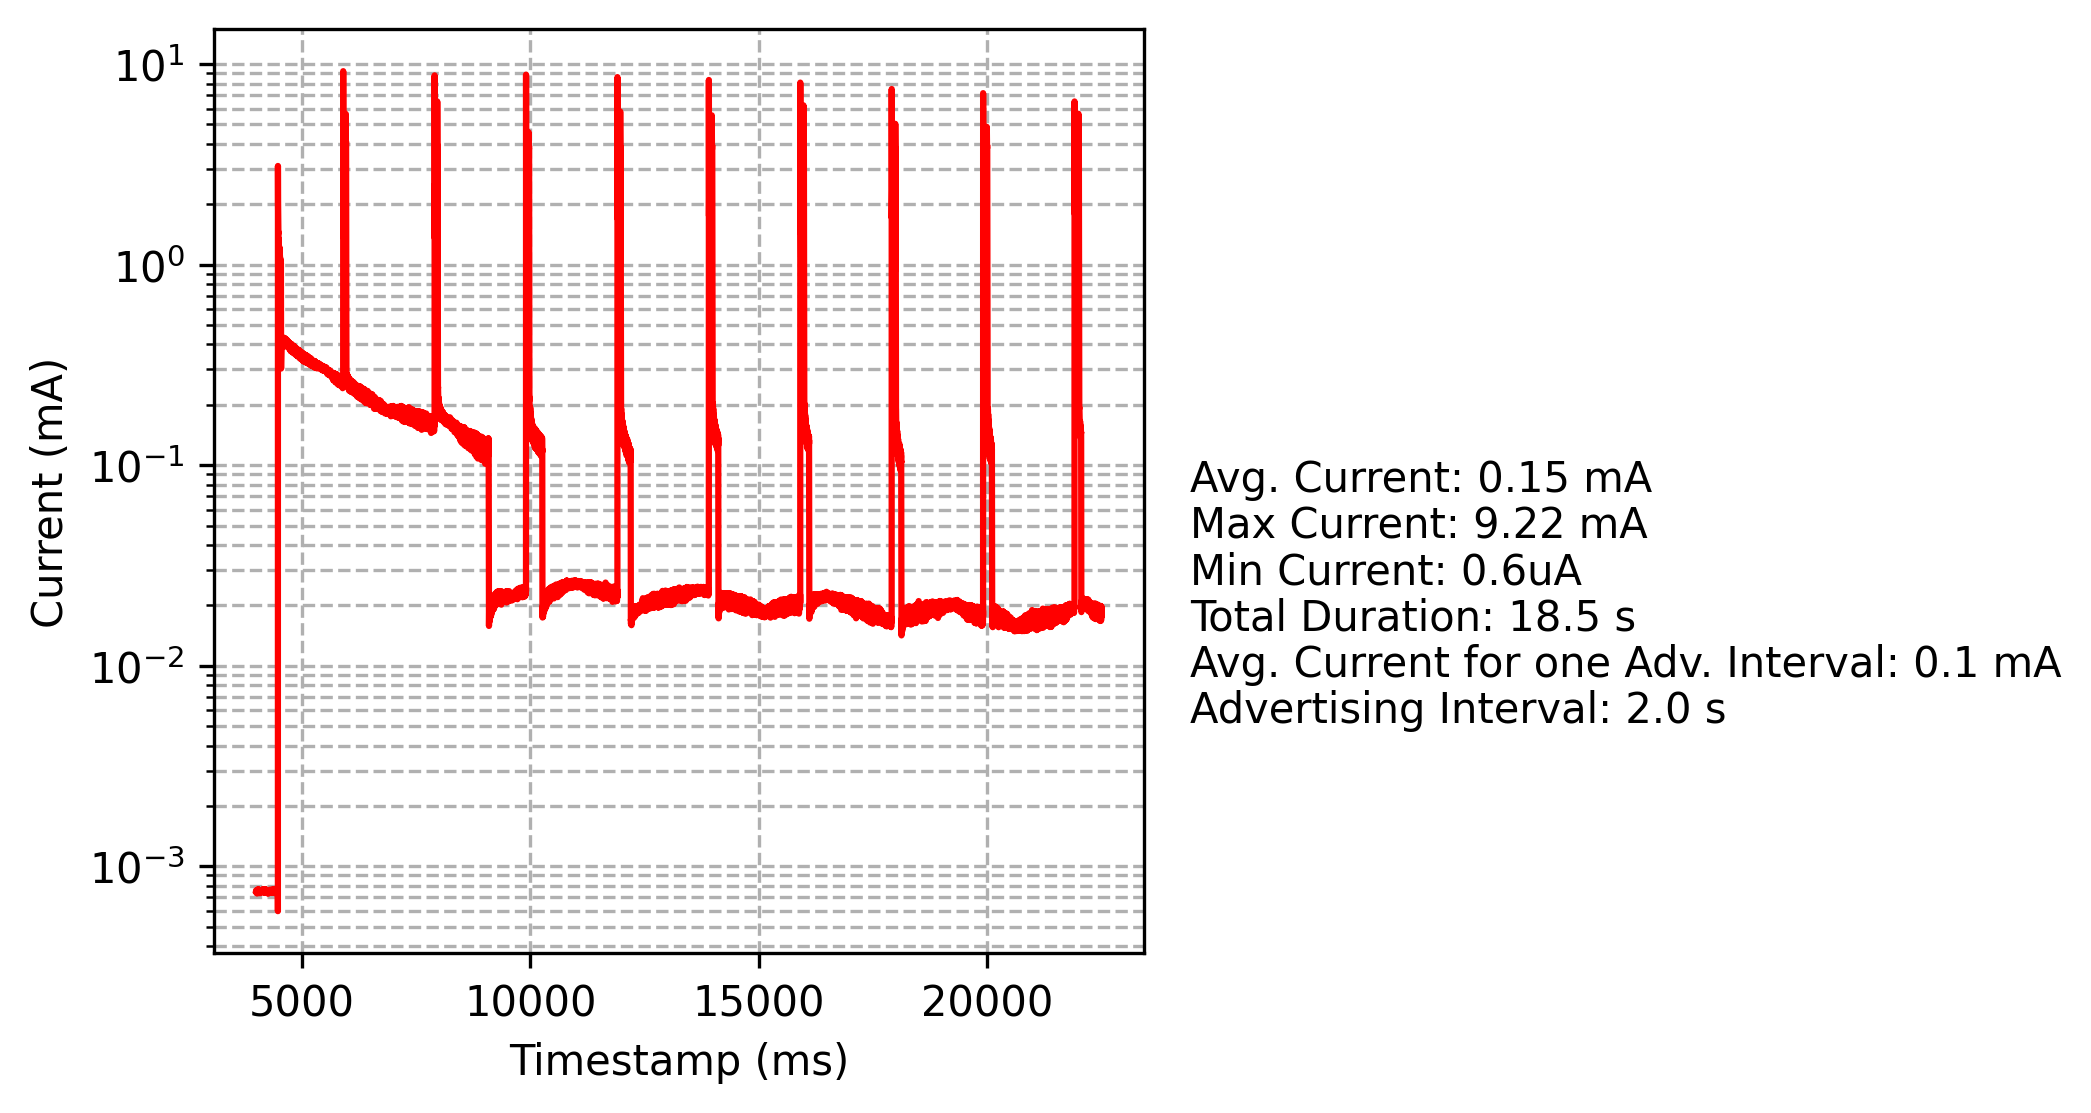
\includegraphics[width=\linewidth]{chapters/Results/Current vs Timestamp - FreeBie Peripheral Medium.png}
        \caption{FreeBie Medium - Peripheral}
        \label{fig:freebie_medium_peripheral}
    \end{subfigure}
    \begin{subfigure}{0.45\linewidth}
        \centering
        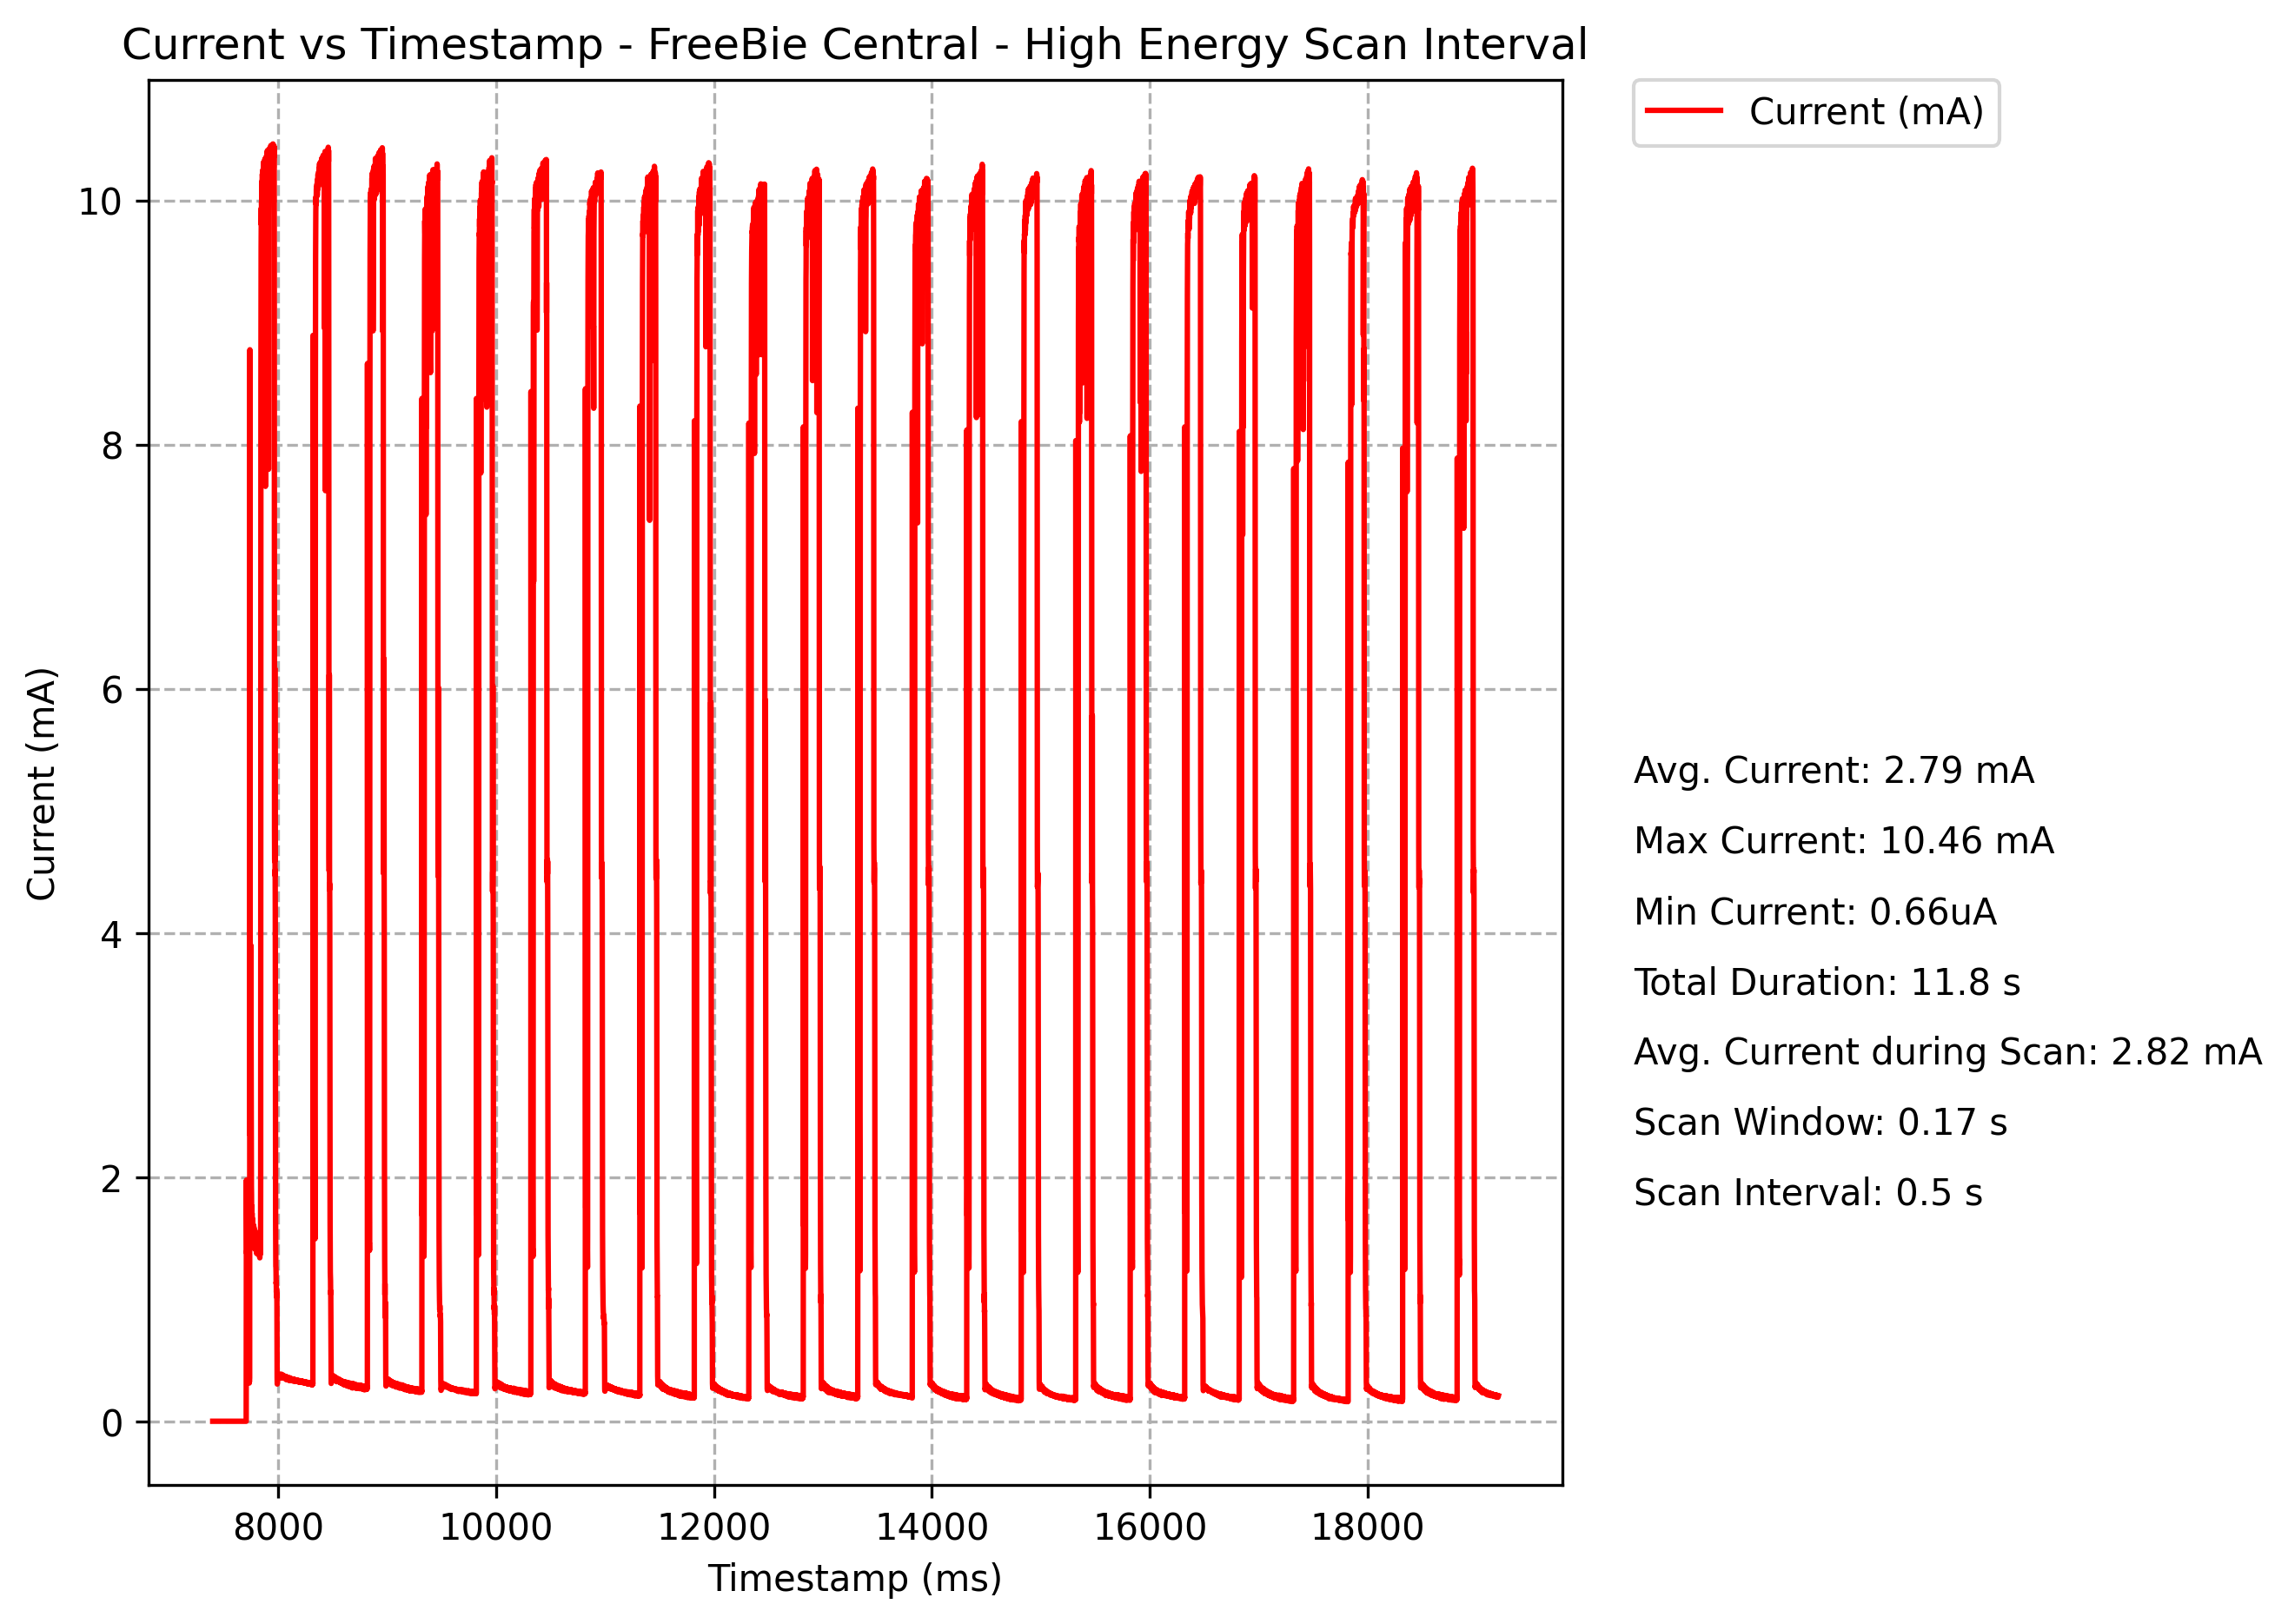
\includegraphics[width=\linewidth]{chapters/Results/Current vs Timestamp - FreeBie Central High.png}
        \caption{FreeBie High- Central}
        \label{fig:freebie_high_central}
    \end{subfigure}\hfill
    \begin{subfigure}{0.45\linewidth}
        \centering
        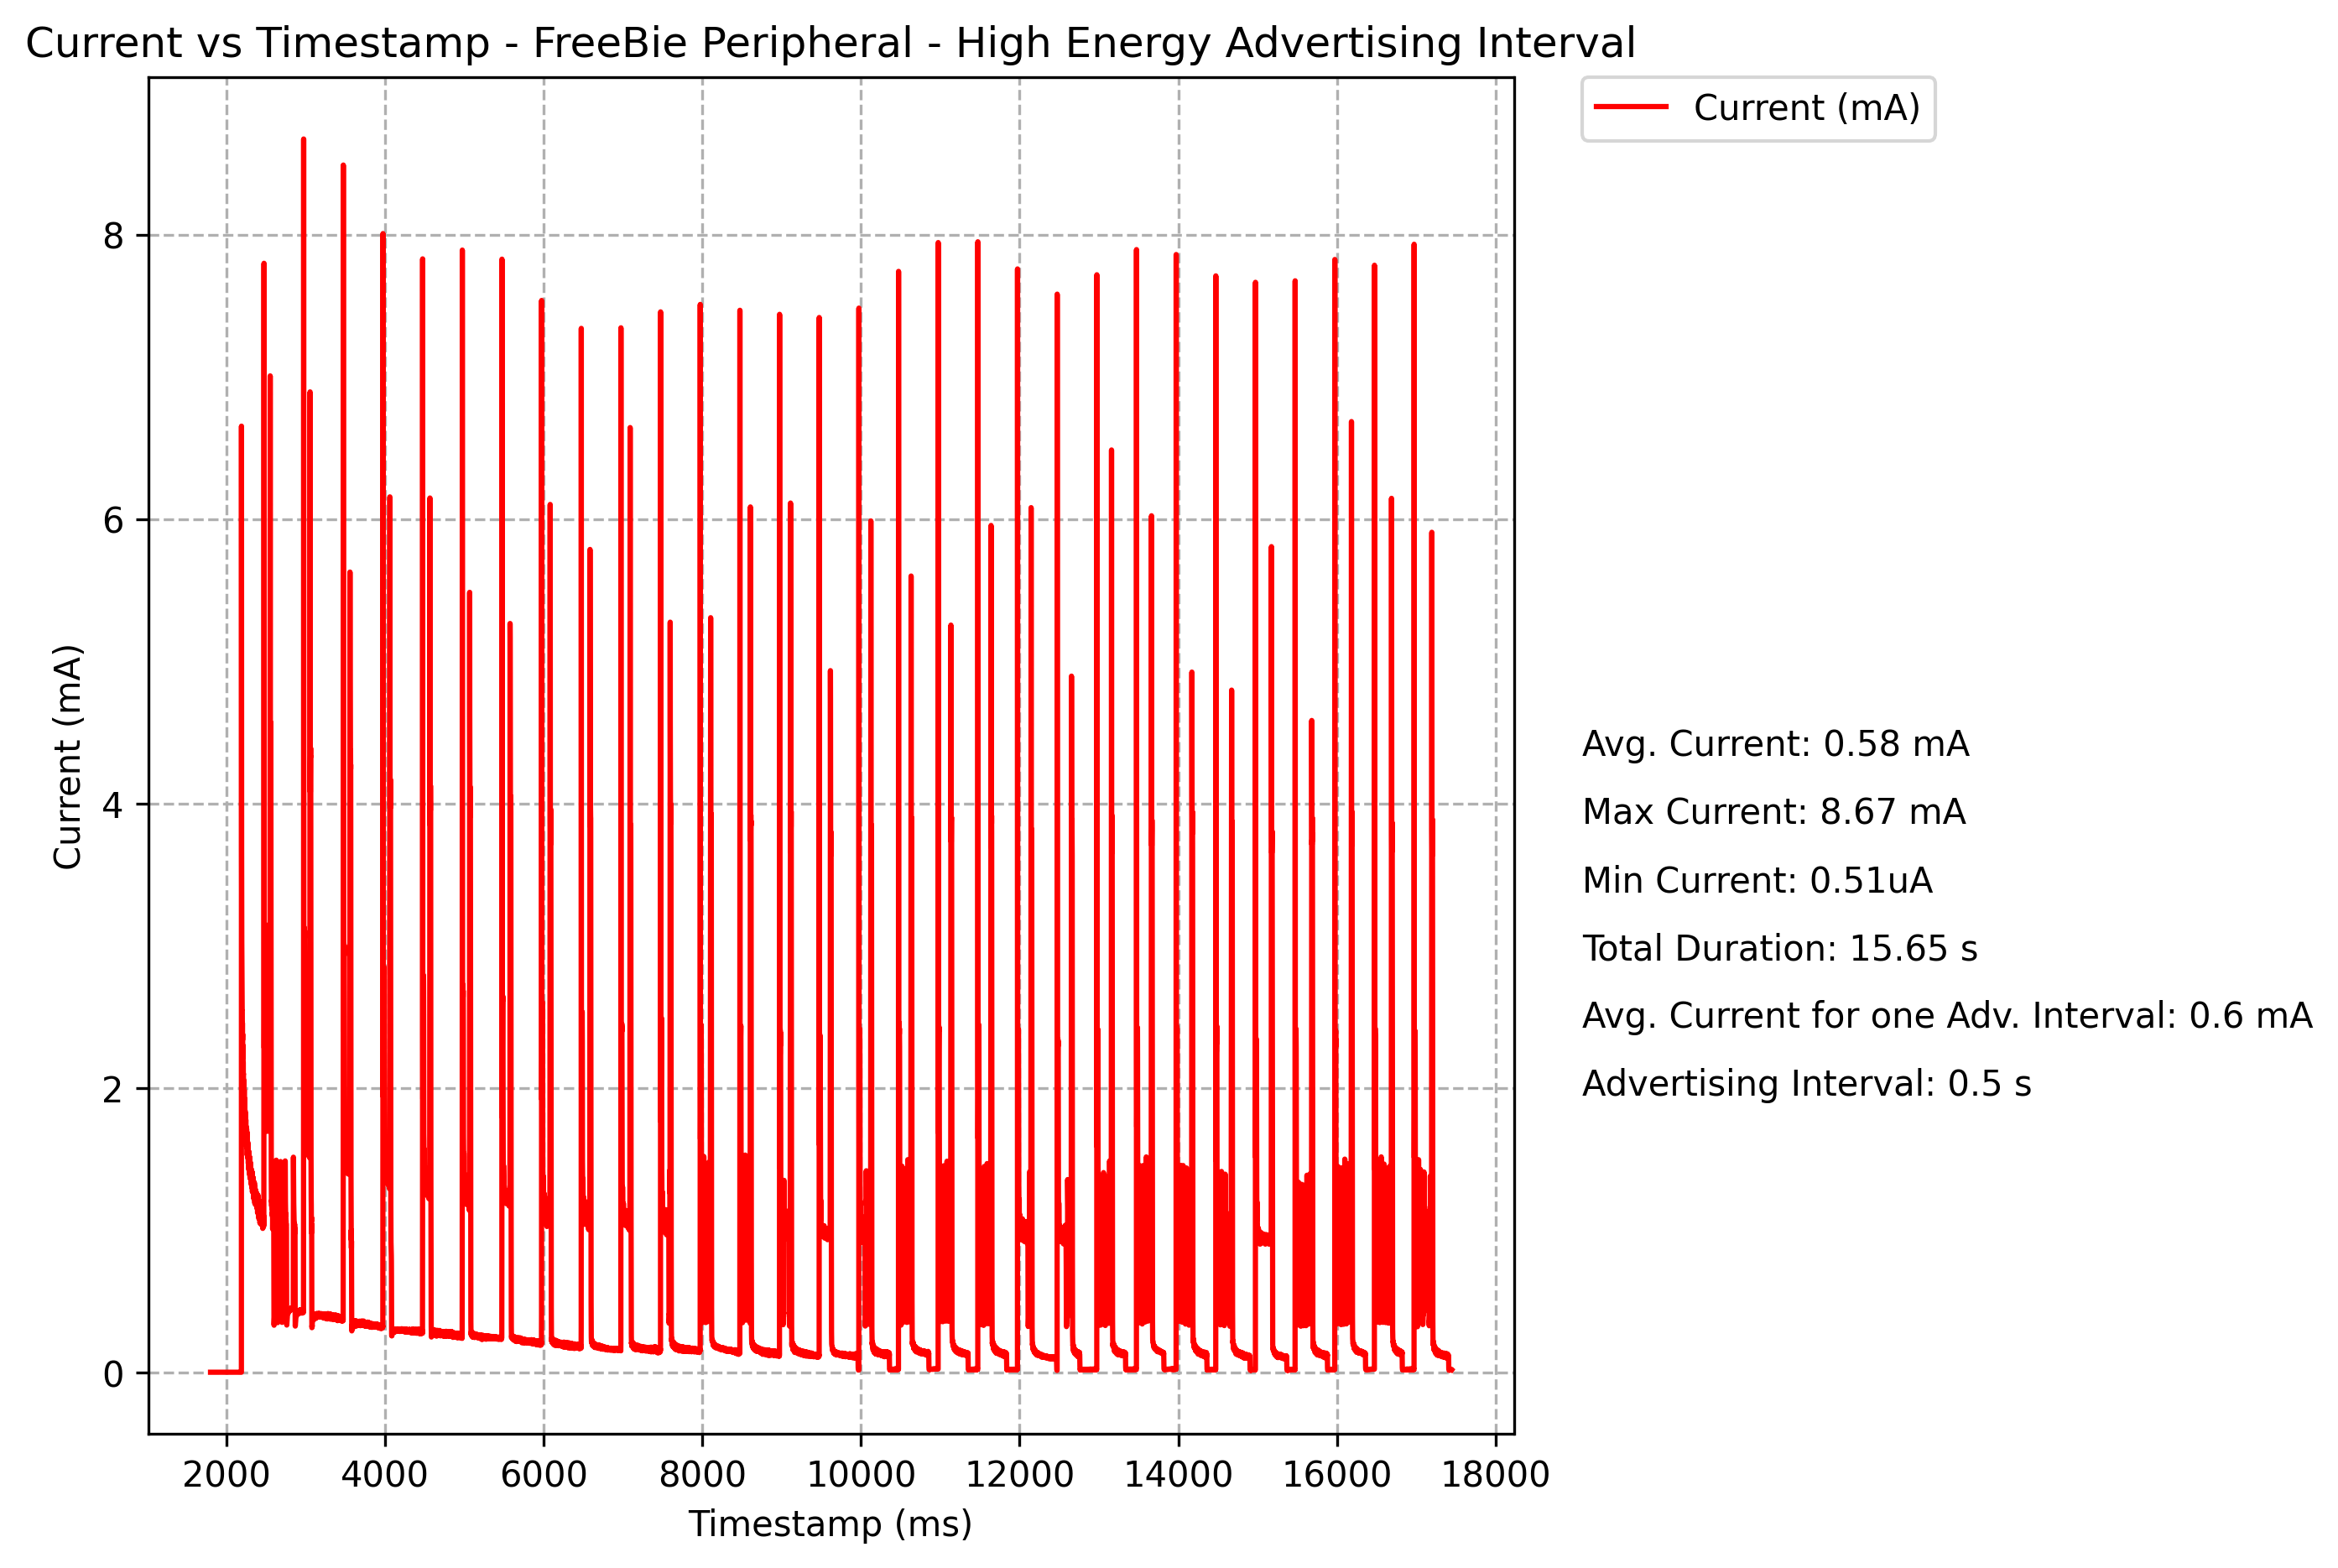
\includegraphics[width=\linewidth]{chapters/Results/Current vs Timestamp - FreeBie Peripheral High.png}
        \caption{FreeBie High - Peripheral}
        \label{fig:freebie_high_peripheral}
    \end{subfigure}
    \caption{Current measurement in idle state without connection establishment for different configurations of reference FreeBie system.}
    \label{fig:current_freebie}
\end{figure}
\begin{table}[t]
\centering
\begin{tabular}{|c|cc|}
\hline
 &
  \multicolumn{2}{c|}{\textit{\textbf{\begin{tabular}[c]{@{}c@{}}Average Current measured\\ in mA\end{tabular}}}} \\ \cline{2-3} 
\multirow{-2}{*}{\textit{\textbf{\begin{tabular}[c]{@{}c@{}}Configuration\\ Name\end{tabular}}}} &
  \multicolumn{1}{c|}{\textit{\textbf{Central}}} &
  \textit{\textbf{Peripheral}} \\ \hline
\cellcolor[HTML]{32CB00}Low    & \multicolumn{1}{c|}{\textit{1.77}} & 0.07 \\ \hline
\cellcolor[HTML]{FFCB2F}Medium & \multicolumn{1}{c|}{\textit{2.78}} & 0.16 \\ \hline
\cellcolor[HTML]{FD6864}High   & \multicolumn{1}{c|}{\textit{2.85}} & 0.6  \\ \hline
\end{tabular}
\caption{Average current measurement using the experimental setup in Section \ref{sec:experimental_setup} for each of the reference system configuration.}
\label{tab:avg_current_freebie}
\end{table}

\noindent Time series voltage measurement plots were generated for each configuration using the same experimental setup discussed in Section \ref{sec:experimental_setup}, as shown in Figure \ref{fig:voltage_freebie}. These plots capture connection establishment during periodic BLE events, with the device entering a sleep state between events, as evidenced by the \(\text{V}_\text{DD\_MCU}\) plot for both Central and Peripheral sides.
\vspace{1\baselineskip}

\noindent Additionally, current trend measured for each BLE configuration in both end devices, as plotted in Figure \ref{fig:current_freebie}, facilitated our comparative energy and power analysis. Then the average current required for BLE connection attempts under various configurations was calculated as illustrated in Table \ref{tab:avg_current_freebie}. 

\subsection{Experimental Setup}
The experimental setup used in this study for comparative assessment is identical to the one stated in Section \ref{sec:experimental_setup}. The experiment recorded the first connection setup time since boot-up for both the CardioSync system and the reference system separately. The measurement of sensor read time is also recorded in the context of the CardioSync system. The experiment was conducted a total of 20 times using the CardioSync device. In the context of the reference system, the experiment is iterated six times for each of the three distinct BLE configurations.
\vspace{1\baselineskip}

\noindent After data collection, the quantification of energy consumption becomes a focal point. The computation of energy expended by the device during each experiment, leading up to connection establishment, is achieved using the formula: \[\text{E(Joules)} = \text{V} \times I_\text{avg} \times T_{\text{Conn}}\].

\noindent The average current $I_\text{avg}$ is measured during distinct phases for both devices, the average voltage supply is 2.6 Volts ($\text{V}$) and $T_\text{Conn}$ corresponds to the time taken to establish a BLE connection since boot up of the device. 
\vspace{1\baselineskip}


\subsection{Connection Setup Time Comparison}
\begin{figure}[t]
    \centering
    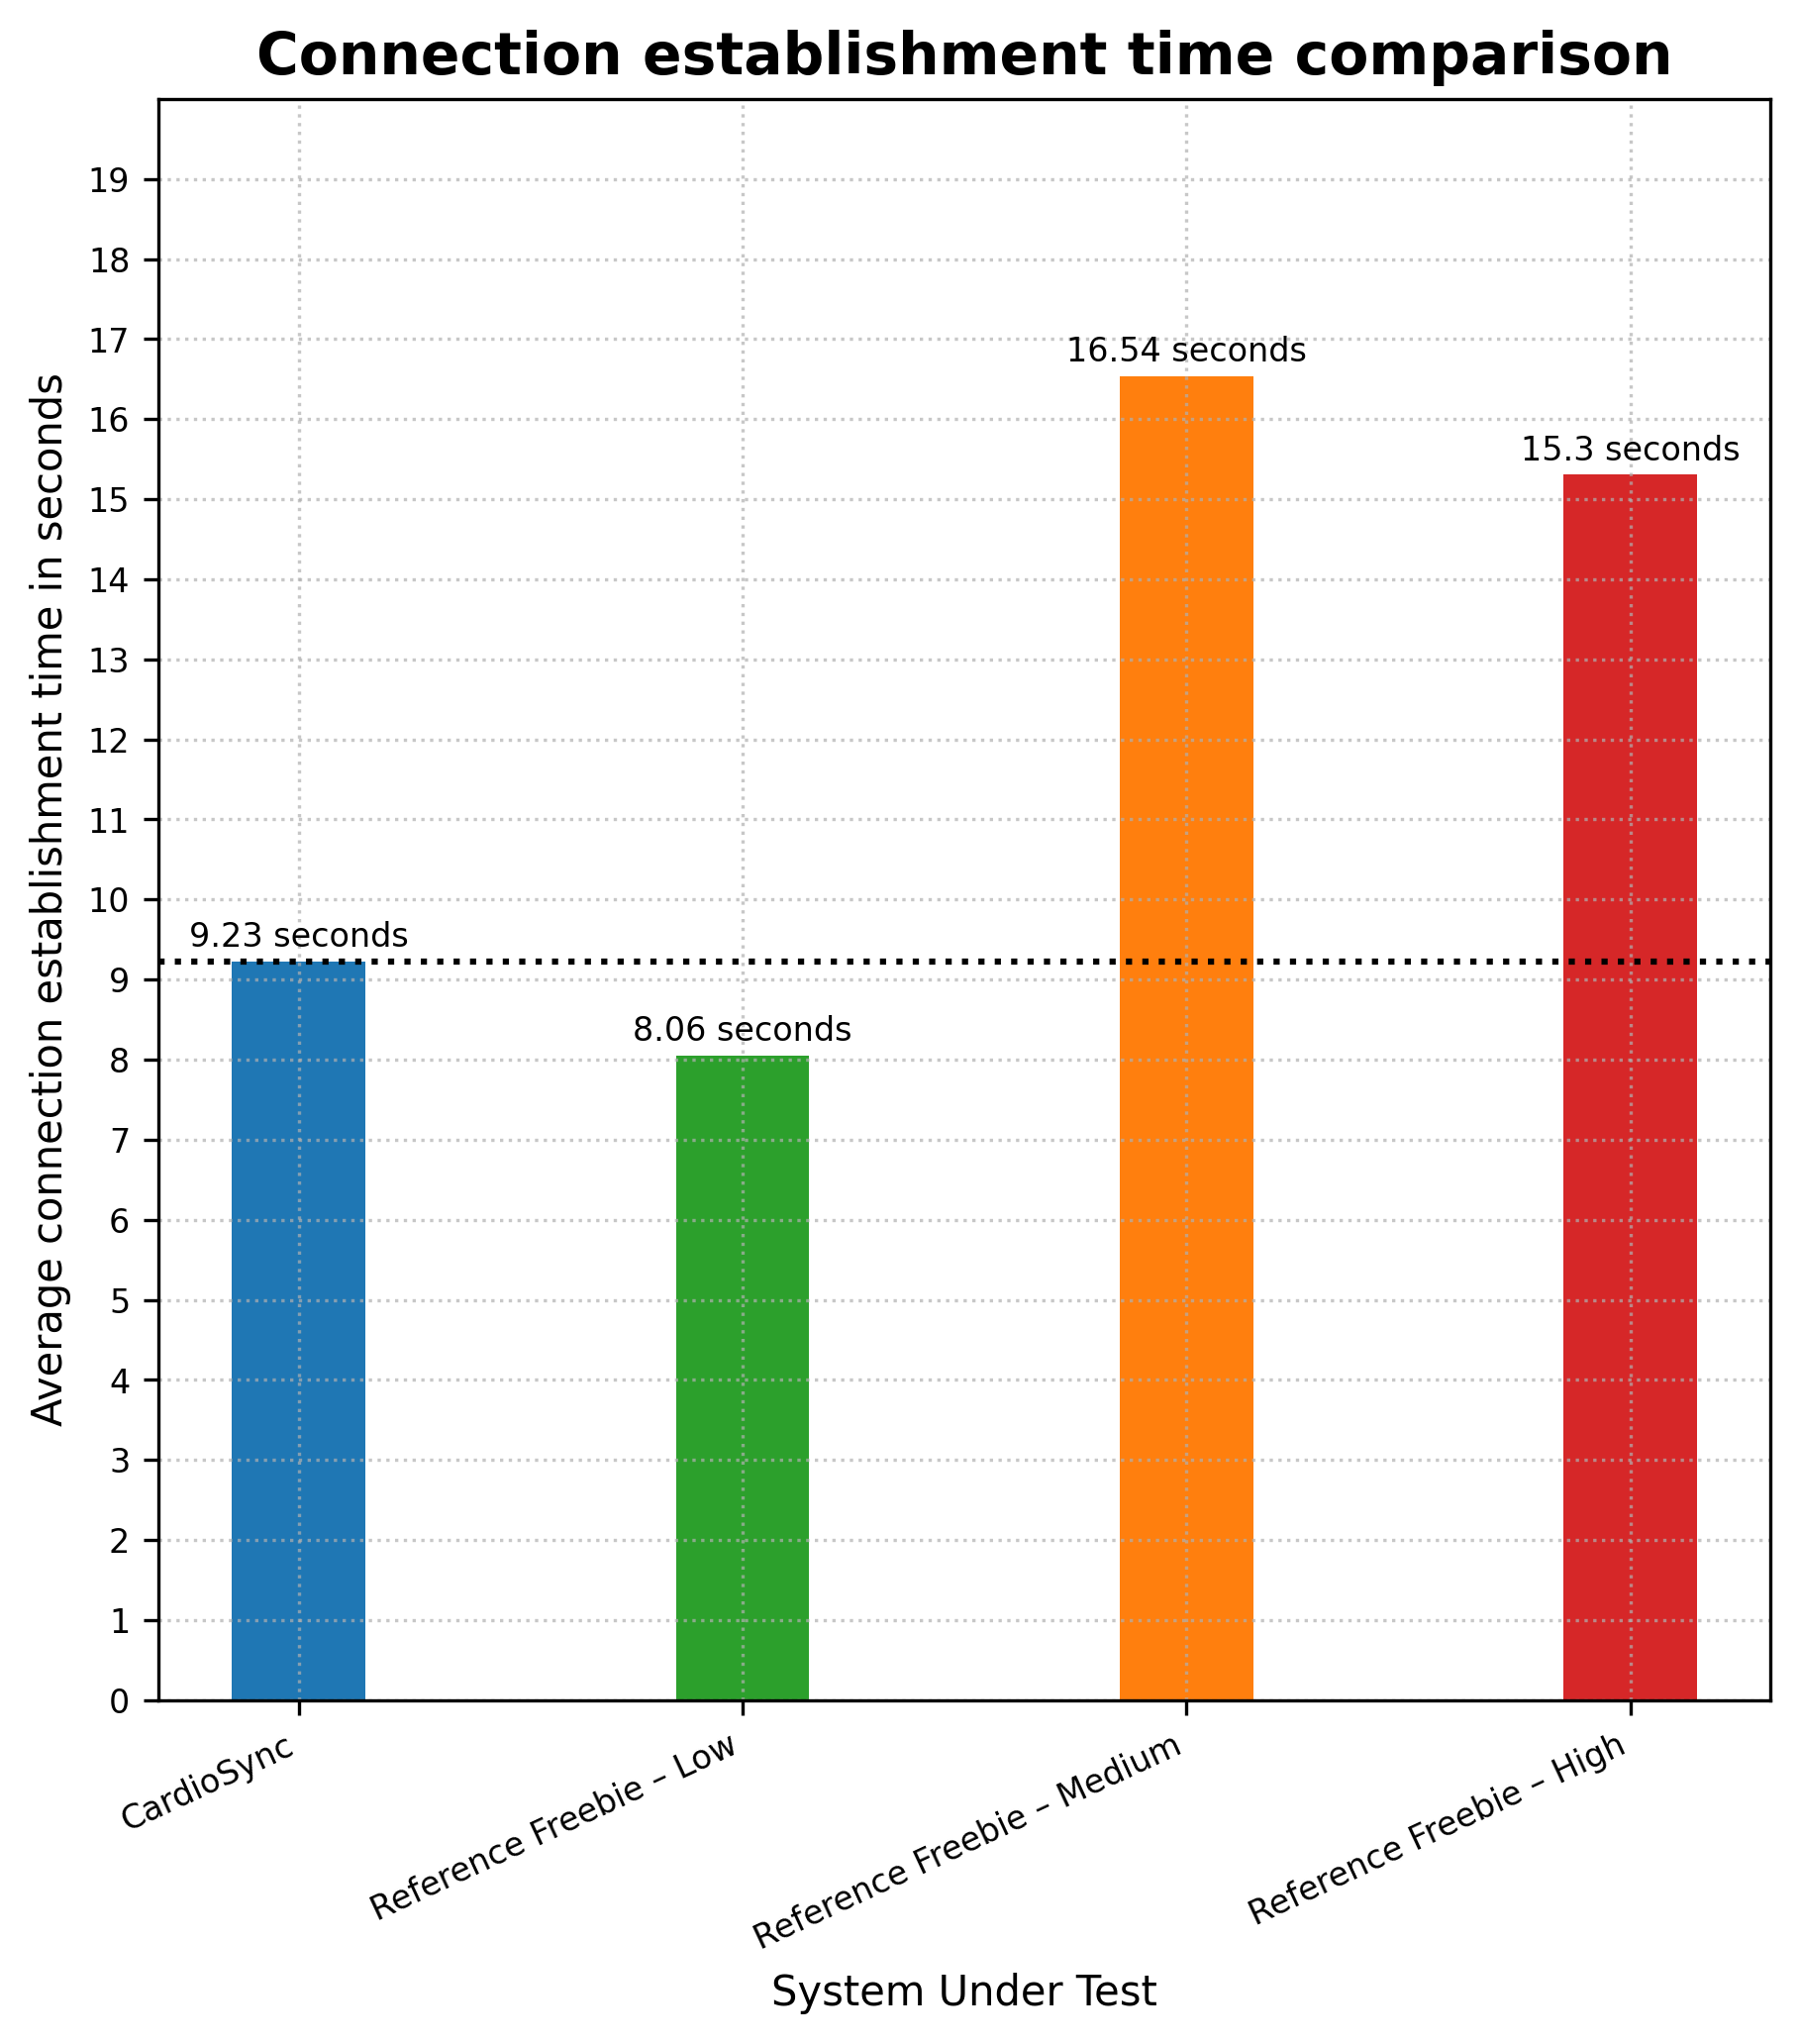
\includegraphics[width=0.7\linewidth]{chapters/Results/Connection_time_comparison.png}
    \caption{Comparison of average BLE connection establishment time for each system.}
    \label{fig:conn_time_comp}
\end{figure}


The bar plot in Figure \ref{fig:conn_time_comp} graphically represents the average connection duration across different systems. Though CardioSync exhibits a slightly longer average connection time compared to the low configuration of the reference FreeBie system, this distinction remains negligible. In contrast, juxtaposing CardioSync with Freebie Medium and FreeBie High configurations reveals a notable improvement in connection efficiency. Impressively, CardioSync achieves an average connection time \textbf{1.79 times faster than FreeBie medium and 1.65 times faster than FreeBie high}.
\vspace{1\baselineskip}

\noindent These insights offer valuable perspectives when considering practical real-world scenarios in the specific contexts chosen to represent the FreeBie reference systems:

\begin{itemize}
    \item \textbf{Limited-Energy Scenario (FreeBie Low):} CardioSync's connection time efficiency, though slightly longer, positions it as a promising solution for scenarios with stringent energy constraints.
    
    \item \textbf{Balanced-Energy Scenario (FreeBie Medium):} CardioSync's significantly faster connection time underscores its potential for enhancing user experiences in fitness tracking devices, where both energy resources and connection efficiency are crucial.
    
    \item \textbf{Abundant-Energy Scenario (FreeBie High):} CardioSync's impressive speed advantage makes it well-suited for scenarios prioritising connection efficiency due to surplus energy availability.
\end{itemize}


\subsection{Energy Consumption Comparison}
\begin{figure}[t]
    \centering
    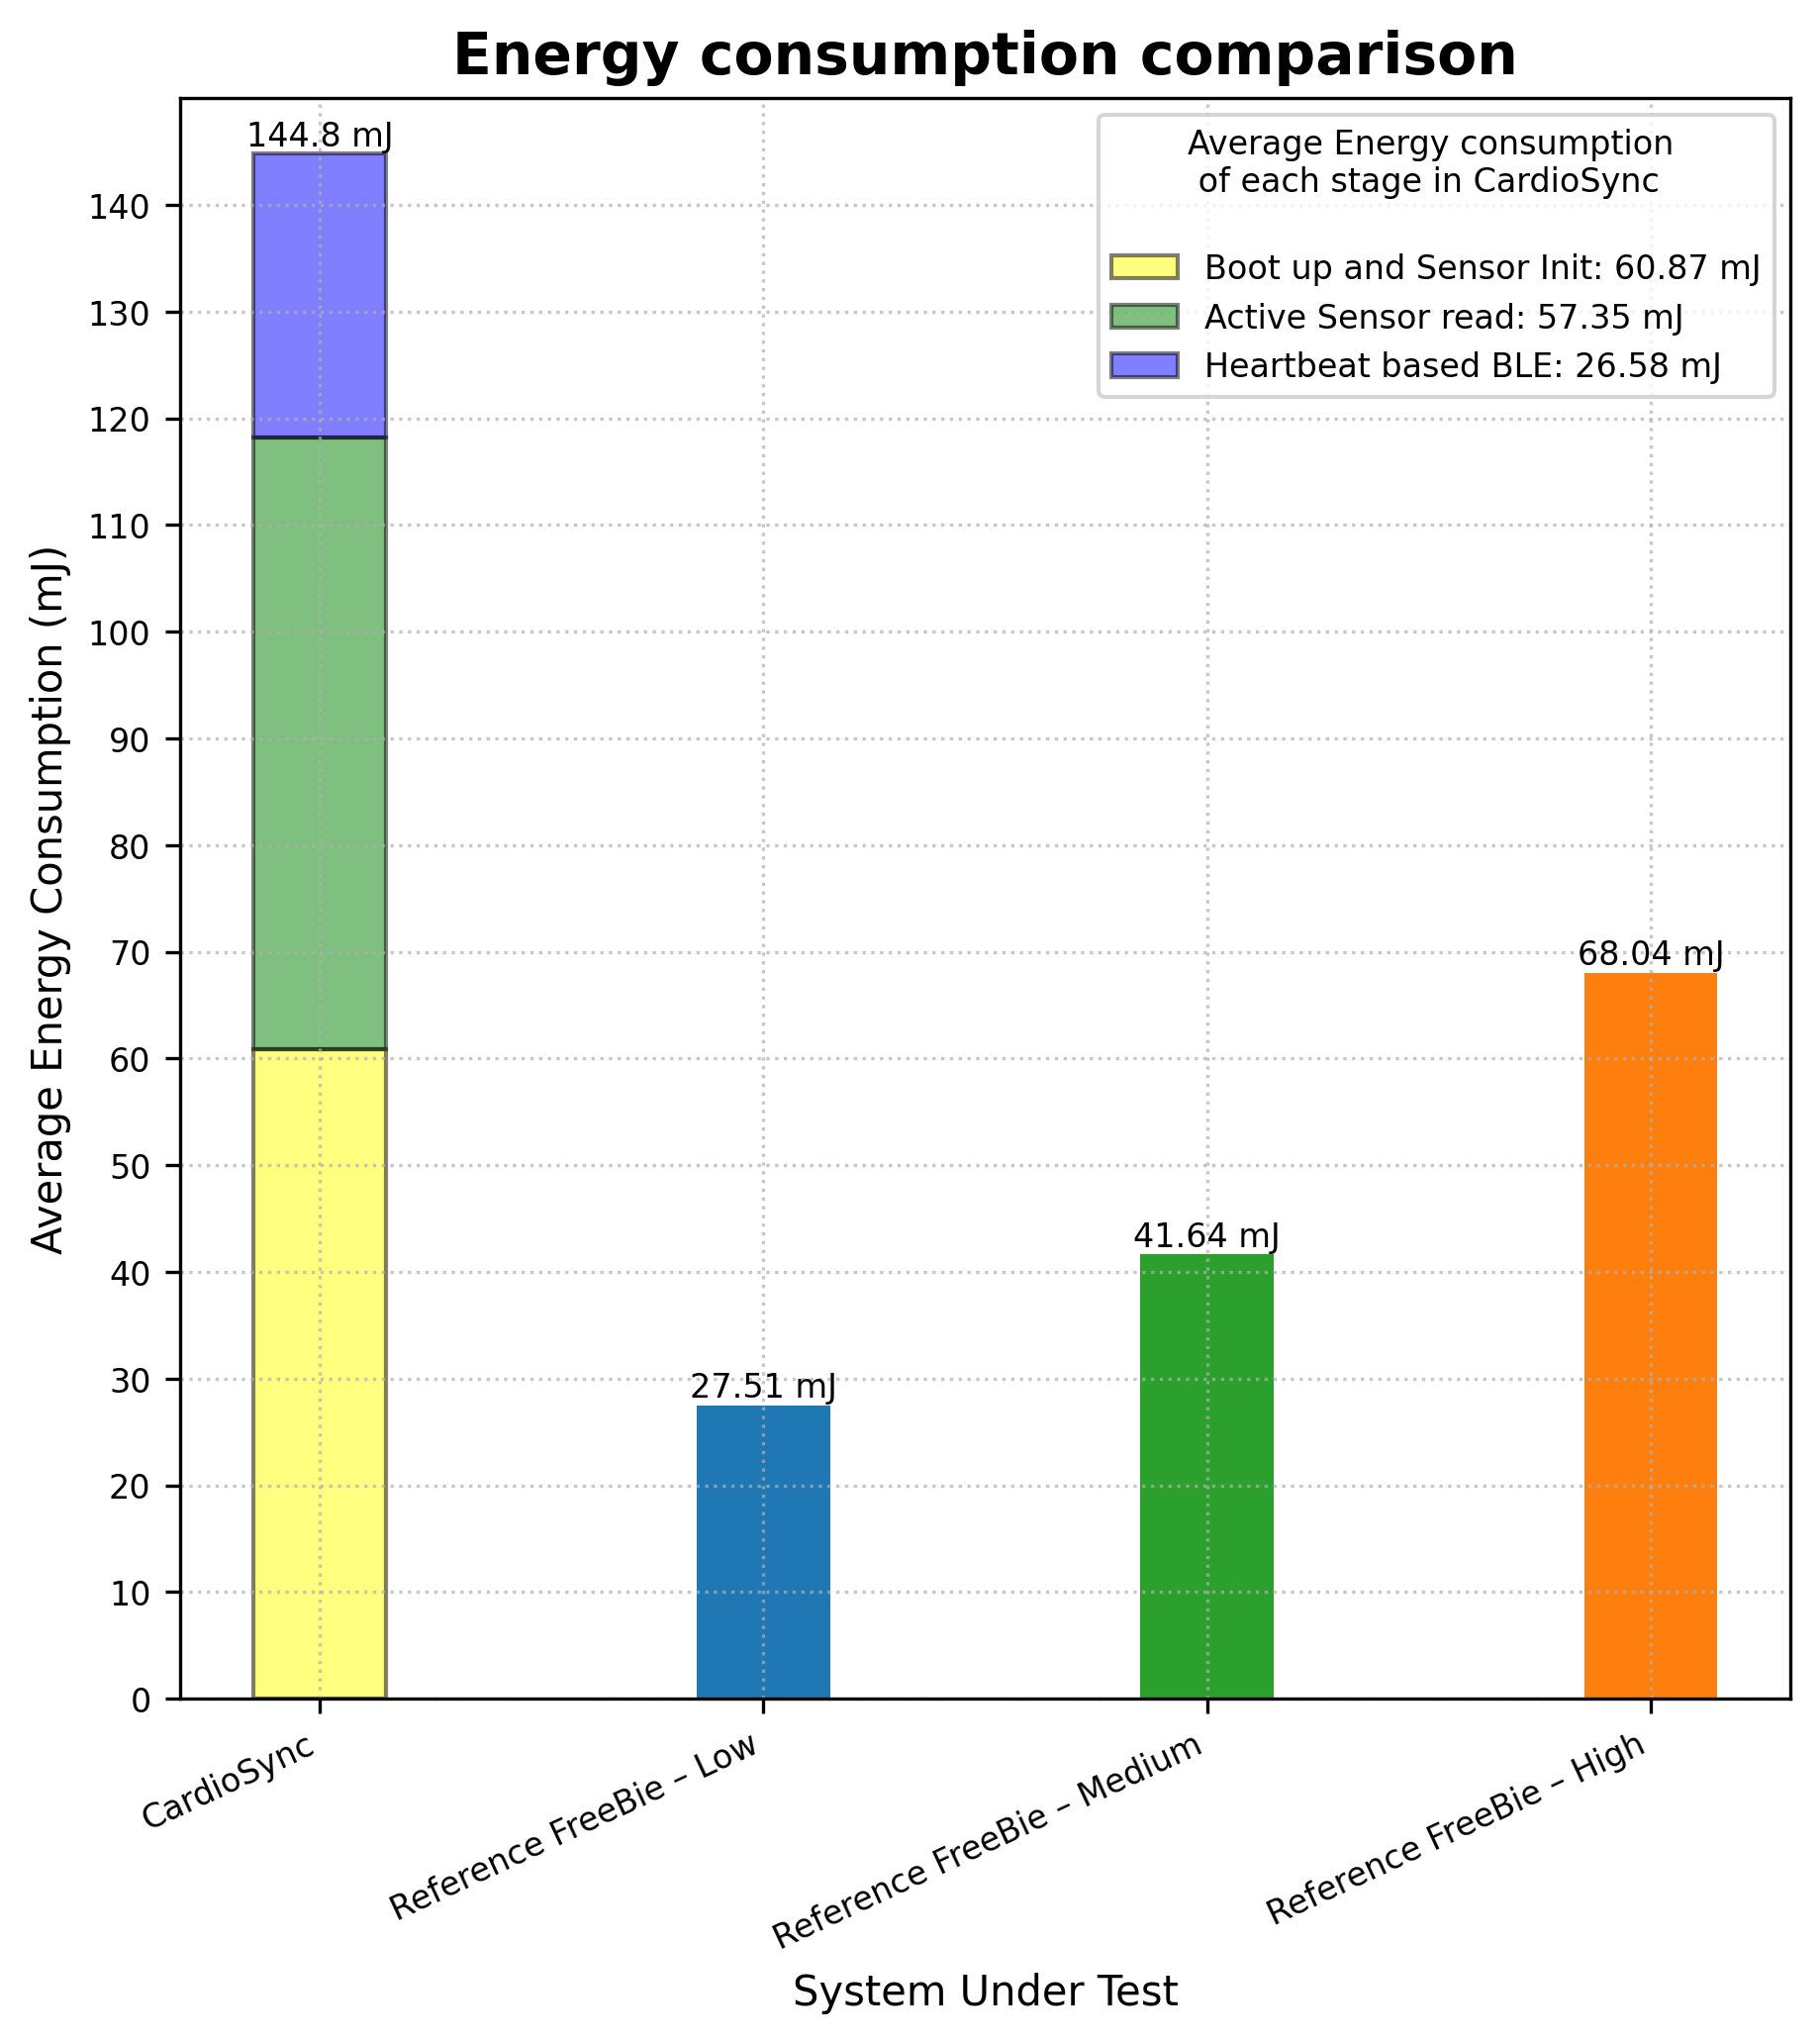
\includegraphics[width=0.7\linewidth]{chapters/Results/Energy_comparison.png}
    \caption{Comparison of average energy consumed till connection setup for each system}
    \label{fig:energy_comp}
\end{figure}

\noindent The bar chart depicted in Figure \ref{fig:energy_comp} provides an illustrative view of the average energy expended to establish a connection for each system. Notably, CardioSync records an average energy consumption of 144.8 mJ, encompassing the cumulative energy consumption from boot-up, sensor initialisation, the "Read and Synchronise" phase, and the "Sleep and Synchronise" phase. The partitioning of this energy consumption into distinct phases is depicted in the bar chart, showcasing the distribution of energy allocation for comprehensive insight. As anticipated, the "Sleep and Synchronise" consumes energy of 26.58 mJ, which is more similar to the energy expended by Naive FreeBie design with a low configuration. This confirms that sensor initialisation and active sensor reading, which employs a polling method, are active energy-consuming phases. In contrast, the reference FreeBie systems exhibit significantly lower energy expenditures—27.51 mJ for FreeBie Low, 41.64 mJ for FreeBie Medium, and 68.04 mJ for FreeBie High.
\vspace{1\baselineskip}

\noindent Comparison of these results reveals that CardioSync consumes notably more energy compared to the reference FreeBie systems. This distinction is particularly evident when compared to FreeBie Low, where CardioSync's energy consumption is around \textbf{5.263 times higher}. Similarly, when contrasted with FreeBie Medium and FreeBie High, CardioSync's energy consumption is \textbf{3.48 and 2.13 times higher}, respectively.
\vspace{1\baselineskip}

\noindent This observed energy disparity aligns with the inherent characteristics of CardioSync, where the integration of the MAX30102 sensor introduces increased energy consumption as a trade-off for improved synchronisation and connection efficiency. Also in the context of the scenarios chosen for the FreeBie reference systems:

\begin{itemize}
    \item \textbf{Limited-Energy Scenario (FreeBie Low):} CardioSync's higher energy consumption aligns with scenarios where energy constraints are paramount, raising questions about its feasibility in such settings.
    
    \item \textbf{Balanced-Energy Scenario (FreeBie Medium):} In scenarios like fitness trackers, where energy resources are limited, the energy efficiency of CardioSync becomes a crucial consideration for extended device functionality. This is particularly important when connection setups fail for extended periods, despite CardioSync demonstrating its ability to operate with intermittent power sources.
    
    \item \textbf{Abundant-Energy Scenario (FreeBie High):} While CardioSync's energy consumption is higher, its speed advantage suggests suitability for scenarios where connection efficiency is prioritised due to surplus energy availability.
\end{itemize}

% \subsection{Power Comparison}
% \begin{figure}[t]
%     \centering
%     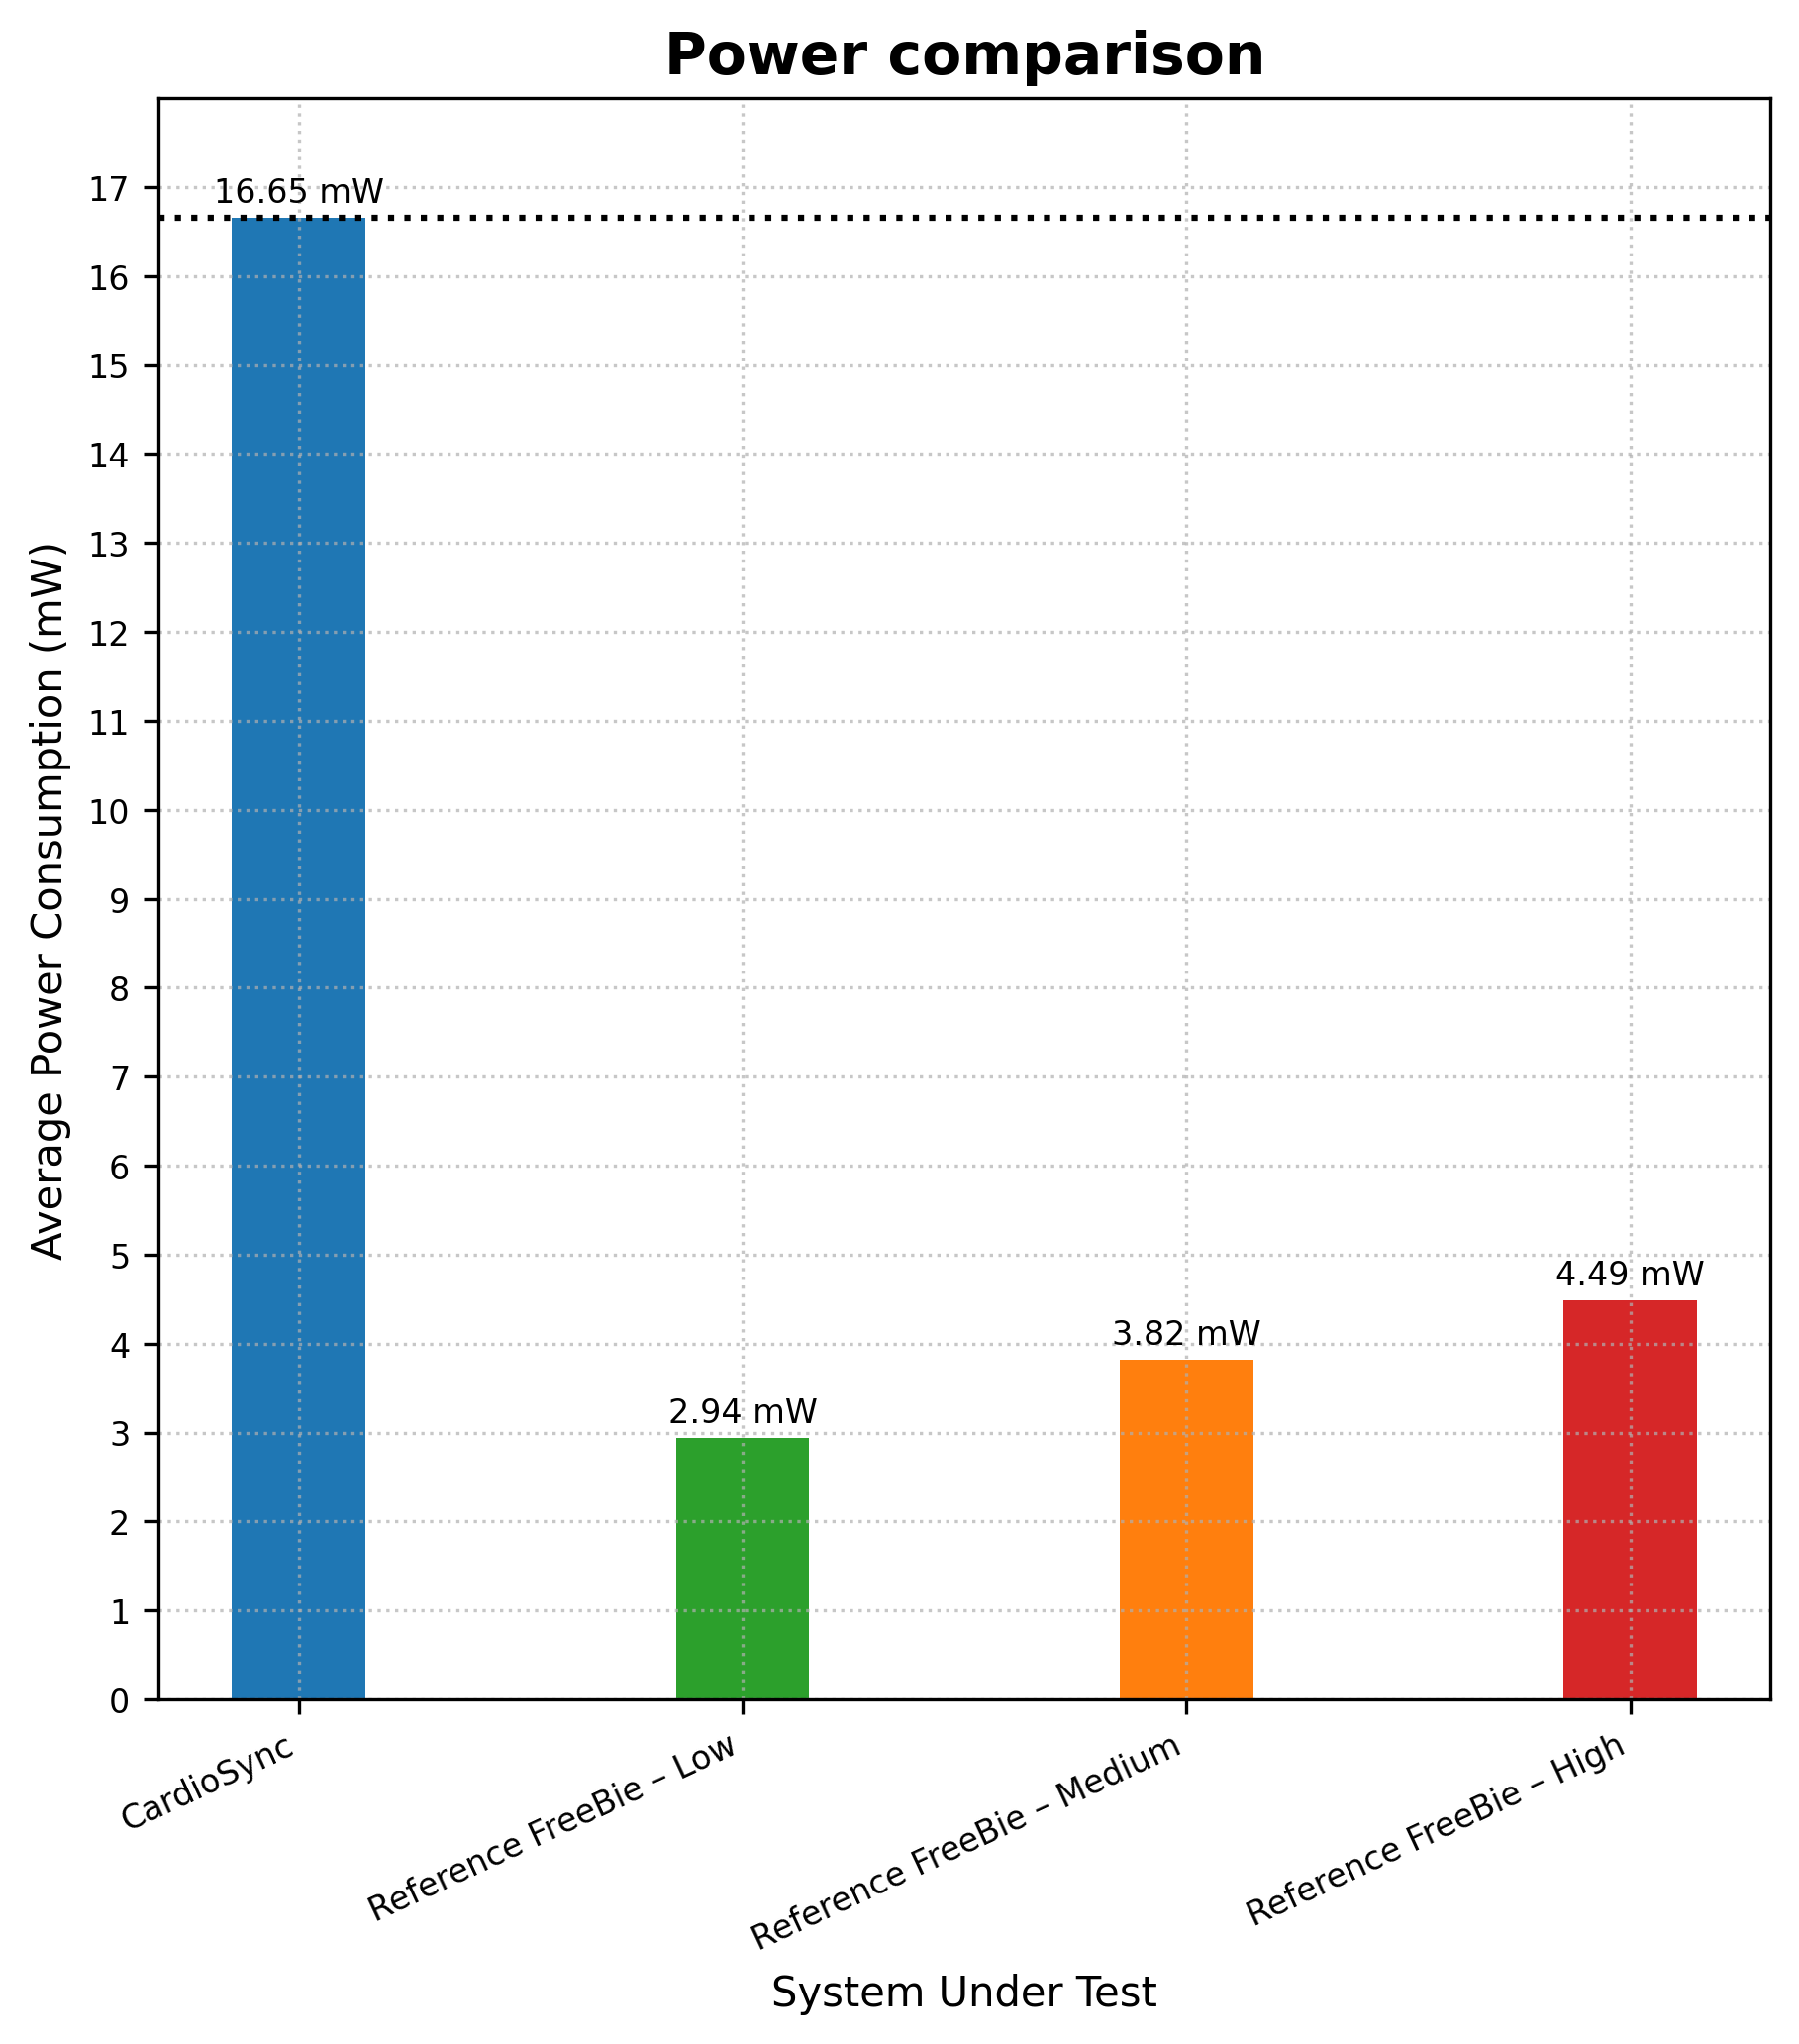
\includegraphics[width=0.7\linewidth]{chapters/Results/Power_comparison.png}
%     \caption{Bar plot showing Average power consumed till connection setup for each system for comparison}
%     \label{fig:power_comp}
% \end{figure}

% \noindent The bar chart depicted in Figure \ref{fig:power_comp} offers a visual representation of the average power expended to establish a connection for each system. Comparing these outcomes underscores that CardioSync consumes significantly more power when compared to the reference FreeBie systems. In comparison to FreeBie Low, CardioSync's power consumption is \textbf{5.66 times higher}. Similarly, in relation to FreeBie Medium and FreeBie High, CardioSync's power consumption is \textbf{4.36 and 3.70 times higher}, respectively. This power discrepancy mirrors the energy consumption pattern observed earlier and is congruent with the inherent trade-offs of the CardioSync system.


\subsection{Understanding Connection Setup Vs. Power}
\begin{figure}[t]
    \centering
    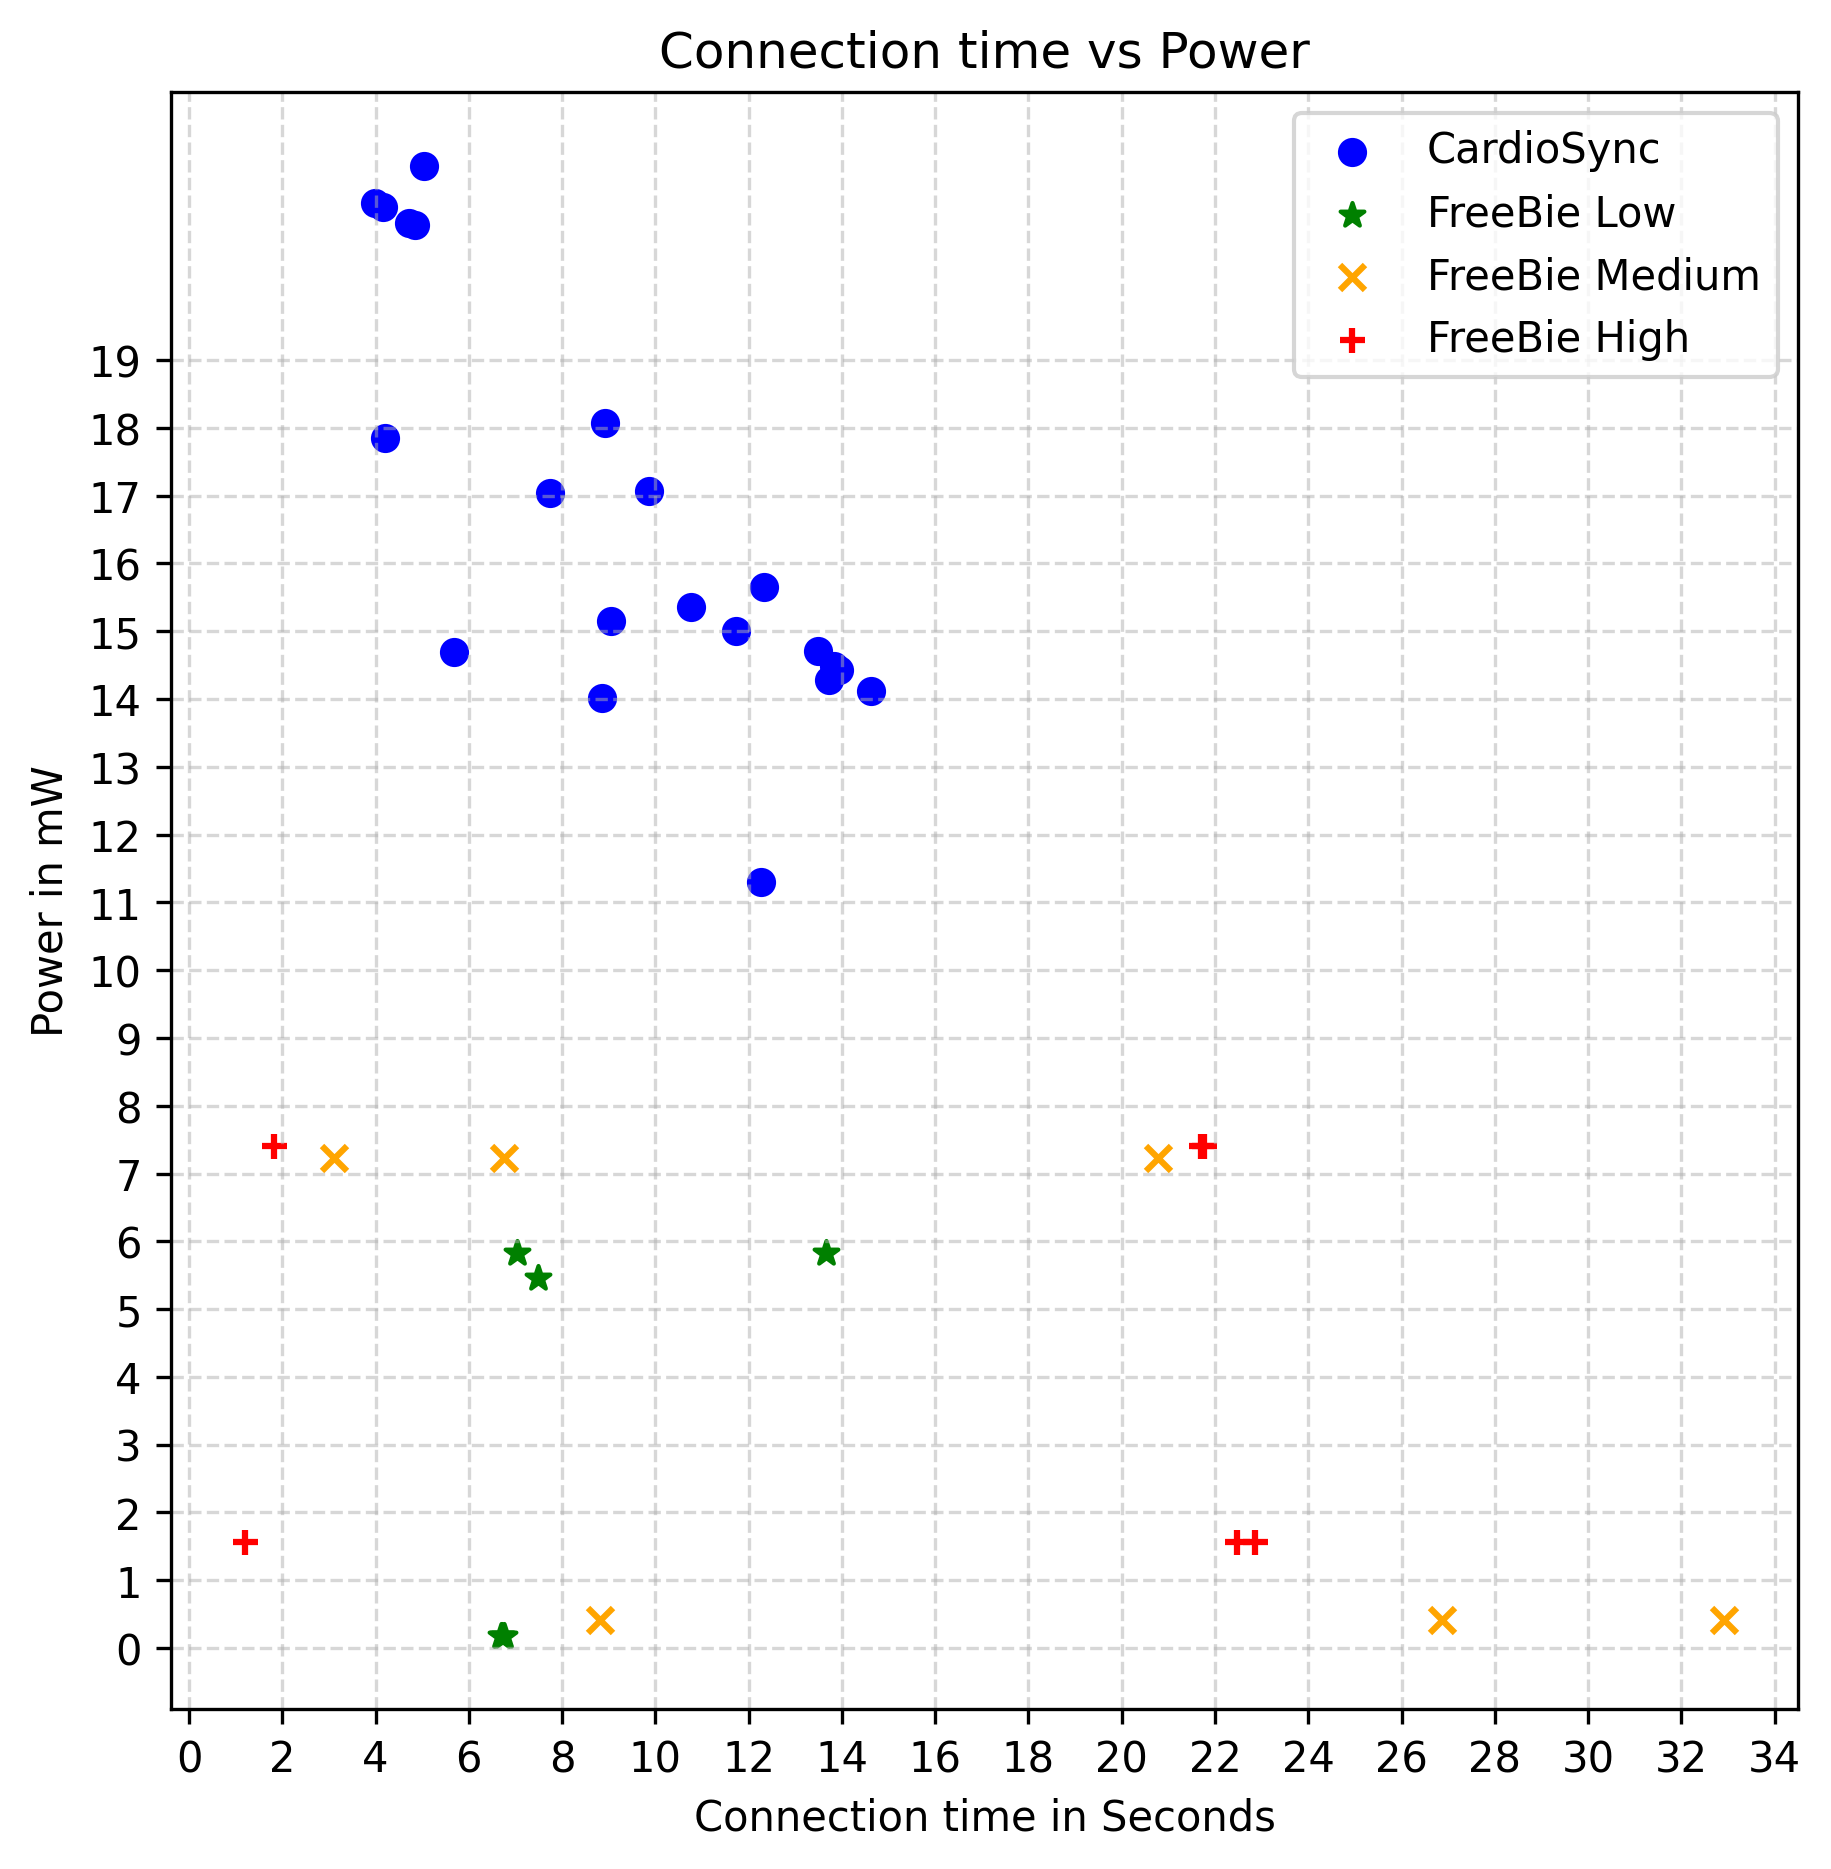
\includegraphics[width=0.7\linewidth]{chapters/Results/Scatter_plot.png}
    \caption{Scatter plot showing Connection time Vs. Power}
    \label{fig:scatter_conn_power}
\end{figure}

\noindent Figure \ref{fig:scatter_conn_power} presents an insightful juxtaposition of connection time against power consumption for both the CardioSync and reference FreeBie systems. Notably, the distribution of experimental data points for the CardioSync system predominantly converges in the upper left quadrant of the graph. In contrast, the scatter plot depicting the reference FreeBie system showcases a more dispersed arrangement of data points, spanning across the lower half of the graph.
\vspace{1\baselineskip}

\noindent This disparity in the distribution of data highlights a pivotal distinction between the two systems. While the CardioSync system exhibits greater power consumption, it consistently achieves expedited connection times. In contrast, the reference FreeBie system, characterised by its asynchronous nature, demonstrates a wider range of connection times. This inconsistency in connection times, despite relatively lower power consumption, highlights the challenges inherent in achieving synchronisation within the battery-less FreeBie architecture.
\vspace{1\baselineskip}

\noindent In essence, the scatter plot serves as a visual testament to the trade-offs between power consumption and connection time. The CardioSync system, which has denser data points in the upper left quadrant, is an example of the potential advantages of utilising external synchronisation mechanisms to achieve consistent and effective connection times in a battery-free context.


\section{Discussion of Key Findings}
In this section, we explore the implications and insights stemming from the comparative analysis between the CardioSync framework and the reference FreeBie system, shedding light on their performance and potential trade-offs.

\begin{itemize}
    \item \textbf{Power and Energy Efficiency:} CardioSync demonstrated higher connection time efficiency, counterbalanced by increased power and energy consumption. This is due to the intentional inclusion of the MAX30102 sensor for synchronisation, which inherently demands additional energy. It's worth noting that the energy spent to establish a synchronised reconnection in case of connection timeouts is significantly lower in CardioSync compared to naive reference FreeBie systems.

    \item \textbf{Connection Time and Synchronisation:} CardioSync consistently achieved reduced connection times, while the reference FreeBie system exhibited a wider range of connection times, reflecting its asynchronous nature. Importantly, the readings from the reference system are after intentional synchronisation. Without this, the reference system's BLE advertising and scanning intervals remain asynchronous, rendering it unable to establish connections. In contrast, CardioSync achieves synchronisation effortlessly.

    \item \textbf{Trade-Offs and Implications:} CardioSync's higher energy usage, resulting in improved connection times, introduces trade-offs to consider in real-world applications. The dispersed connection times in the reference FreeBie system highlight the difficulty of achieving synchronisation.

\end{itemize}

\noindent In summary, the detailed evaluation of CardioSync against the reference FreeBie system aligns strategically with our research objectives and validates our research goals, effectively enhancing the discourse and possibilities within the battery-less domain.

% Create conclusions
\chapter{Conclusions}
\label{chp:conclusions}

In this thesis, we have introduced the CardioSync framework, a novel solution that addresses a significant limitation in the state-of-the-art intermittent BLE device, FreeBie. The core challenge of achieving true intermittency between two end nodes and forming a reliable BLE network has been successfully overcome through CardioSync. This framework harnesses the capabilities of the low-power heart rate monitoring sensor, to synchronise connection setups between two battery-free nodes, employing the human heart rate as a shared clock pulse. By leveraging the inherent rhythm of the human heart, CardioSync achieves an average connection time that is nearly \textbf{1.8 times faster} compared to the FreeBie model's asynchronous periodic connection setup strategy. As promising as this is, it comes with an understandable trade-off of increased power demand for the connection setup due to sensor integration. The CardioSync framework demands \textbf{3.70 times more power} than reference FreeBie model.
\vspace{1\baselineskip}

\noindent This novel approach paves the way for a wide range of applications, especially in the field of Body Sensor Networks (BSN). The ability to establish connections between battery-free devices without relying on external power sources holds immense promise for healthcare monitoring, environmental sensing, and beyond. Looking ahead, the implications of the CardioSync framework on wearable health monitoring and IoT are significant. Its success opens avenues for more efficient and sustainable IoT deployments, reducing the environmental impact of battery disposal. With each synchronised connection established by CardioSync, we move closer to realising a more connected and sustainable world.

% Create future work
\chapter{Future Work}
\label{chp:futurework}

While this thesis has presented an advancements in the field of battery-less embedded systems and synchronisation, there are several avenues for further exploration and improvement. The following outlines potential directions for future research

\begin{itemize}
    \item \textbf{Fine-Tuning Sensor Utilisation}: Further optimising the utilisation of the heart rate sensor holds the potential for increased energy efficiency. The chosen sensor configurations detailed in Section \ref{sec:sensor_config} are already finely balanced to conserve energy while excelling in heart rate detection. However, there remains room for additional optimisation through adjustments in duty cycle and the bit resolution of the ADC. Additionally, when measuring current while the sensor is interfaced, a noticeable residual current was detected in the Power Profiler Kit \cite{2023Power}. Addressing this could involve employing a power switch for the sensor's $V_\text{DD}$ line, fully deactivating it when the MCU enters an OFF state. This approach has the potential to yield modest reductions in energy consumption.

    \item \textbf{Adaptive Synchronisation Strategies:} Developing dynamic synchronisation strategies that can adapt to connection setup failures by intelligently adjusting parameters such as widening the scan window or prolonging the advertising duration. This would involve monitoring for connection attempts and failure counts in post processing stage of algorithm and adjusting synchronisation intervals accordingly.

    \item \textbf{Exploring Different Sensor Platforms: }While the chosen heart rate sensor - MAX30102 has proven effective, considering alternative sensor platforms could provide insights into sensor energy efficiency and accuracy trade-offs. Exploring newer sensor technologies could yield novel opportunities.

    \item \textbf{Real-World Deployments and Practical Testing:} Conducting real-world deployments and testing CardioSync in various scenarios, including wearable applications or IoT systems, would validate its performance outside controlled environments. Practical challenges and optimisations can be explored.
\end{itemize}

% Create bibliography
\bibliographystyle{plain} % Please do not change the style of bibliography (yes, it should be `plain`)
\bibliography{bib/MyMScTUDESThesisBibFile} % remove "../" before "bib" if you compile directly in Overleaf or in your favourite local LaTeX distribution

% Create appendix
\appendix
\chapter{APPENDIX TITLE}
\label{app:appendix_a}

Appendix body.

\end{document}
